\documentclass[11pt, a4paper]{article}
\usepackage{graphicx}
\usepackage[a4paper, margin=2cm]{geometry}
\usepackage{fontspec}
\usepackage[english, vietnamese, bidi=basic, provide=*]{babel}
\babelprovide[import, onchar=ids fonts]{vietnamese}
\babelprovide[import, onchar=ids fonts]{english}
\babelfont{rm}{Noto Sans}

\usepackage[normalem]{ulem}
\newcommand{\pk}[1]{\bgroup\ULdepth=1.8pt\uline{#1}\egroup}
\newcommand{\fk}[1]{\bgroup\ULdepth=1.8pt\dashuline{#1}\egroup}
\newcommand{\pkfk}[1]{\bgroup\ULdepth=1.8pt\uline{\bgroup\ULdepth=4.0pt\dashuline{#1}\egroup}\egroup}

\usepackage{enumitem}
\setlist[itemize]{label=-, leftmargin=1.5em, itemsep=2pt, topsep=3pt}

\usepackage{tabularx}
\usepackage{array}
\usepackage{booktabs}
\usepackage{amsmath}
\usepackage{amssymb}
\usepackage{hyperref}

\hypersetup{
    colorlinks=true,
    linkcolor=black,
    urlcolor=blue
}

\renewcommand{\tabularxcolumn}[1]{m{#1}}
\newcolumntype{C}[1]{>{\centering\arraybackslash}m{#1}}
\newcolumntype{Y}{>{\centering\arraybackslash}X}
\renewcommand{\arraystretch}{1.2}

\setlength{\parindent}{0pt}
\setlength{\parskip}{5pt}

\begin{document}

\begin{titlepage}
\begin{center}
    {\large \textbf{ĐẠI HỌC QUỐC GIA TP.HCM}}\\[4pt]
    {\large \textbf{TRƯỜNG ĐẠI HỌC KHOA HỌC TỰ NHIÊN}}\\[4pt]
    {\large \textbf{KHOA CÔNG NGHỆ THÔNG TIN}}\\[1.8cm]

    
\includegraphics[width=3.8cm]{hcmus-logo.png}\\[1.5cm]

    {\LARGE \textbf{ĐỒ ÁN THỰC HÀNH}}\\[8pt]
    {\large \textbf{Học phần: CSC12002 -- Cơ sở dữ liệu nâng cao}}\\[6pt]
    {\large \textbf{Môi trường: Microsoft SQL Server}}\\[1.5cm]

    \rule{\textwidth}{1.2pt}\\[0.4cm]
    {\LARGE \textbf{HỆ THỐNG FITLIFE HUB}}\\[6pt]
    {\Large \textbf{Báo cáo Tổng kết Đồ án (Giai đoạn 1 \& Giai đoạn 2)}}\\[0.2cm]
    \rule{\textwidth}{1.2pt}\\[1.2cm]

    {\large \textbf{Mã số đồ án: 2627.ADB.01}}\\[2cm]
\end{center}

\vfill

\hspace{1cm}
\begin{tabular}{ll}
    \textbf{Giảng viên hướng dẫn:} & Hồ Thị Hoàng Vy, Tiết Gia Hồng \\[4pt]
    \textbf{Nhóm thực hiện:} & Nhóm 10 \\[4pt]
    \textbf{Thành viên:} & Bùi Ngọc Minh Huy -- 24120321 \\[2pt]
    & Lê Đình Huy -- 24120324 \\[2pt]
    & Phạm Bá Quốc Huy -- 24120326 \\[2pt]
    & Đinh Tiến Phát -- 24120405 \\
\end{tabular}

\end{titlepage}

\newpage
\renewcommand{\contentsname}{Mục lục}
\tableofcontents
\newpage
\setcounter{page}{1}

\section{Mô tả chi tiết quy trình nghiệp vụ}

\subsection{Quy trình quản lý chi nhánh}
FitLife Hub quản lý nhiều chi nhánh tại các thành phố lớn. Mỗi chi nhánh được định danh bằng mã chi nhánh duy nhất và có các thông tin như tên chi nhánh, địa chỉ, số điện thoại, giờ mở cửa, giờ đóng cửa và các dịch vụ, tiện ích được cung cấp. Khi thành lập chi nhánh mới, người quản lý có quyền thêm thông tin chi nhánh vào hệ thống. Khi có sự thay đổi về địa chỉ, số điện thoại, thời gian hoạt động hoặc danh sách dịch vụ, thông tin tương ứng được cập nhật. Các nghiệp vụ bán hàng, quản lý hội viên, check-in, đặt lịch huấn luyện viên và quản lý nhân sự đều phải xác định chi nhánh liên quan. Hệ thống cho phép ban giám đốc tra cứu danh sách chi nhánh, so sánh doanh thu, đánh giá hiệu quả hoạt động và theo dõi tình hình sử dụng dịch vụ tại từng địa điểm.

\textbf{Dữ liệu liên quan:} Chi nhánh, dịch vụ, nhân viên, hóa đơn, check-in, lịch hẹn PT và tồn kho sản phẩm.

\subsection{Quy trình đăng ký và quản lý hội viên}
Khi khách hàng đăng ký trở thành hội viên, nhân viên lễ tân tiếp nhận thông tin gồm họ tên, số điện thoại, email, số CCCD, giới tính và ngày sinh. Hệ thống kiểm tra các thông tin bắt buộc và những giá trị cần duy nhất, chẳng hạn mã hội viên, số CCCD hoặc số điện thoại nếu quy định nghiệp vụ yêu cầu không trùng lặp. Sau khi đăng ký thành công, hệ thống tạo mã hội viên và ghi nhận ngày đăng ký. Hội viên có thể mua một hoặc nhiều gói dịch vụ tùy theo nhu cầu. Thông tin hội viên được sử dụng trong các nghiệp vụ thanh toán, xác thực quyền vào tập, đặt lịch PT và tích lũy điểm thưởng. Khi hội viên thay đổi số điện thoại, email hoặc thông tin cá nhân, nhân viên có thẩm quyền cập nhật hồ sơ. Hệ thống cần bảo đảm các hóa đơn, lịch hẹn và lịch sử check-in đã phát sinh vẫn liên kết đúng với hội viên, không bị mất khi thông tin cá nhân được chỉnh sửa.

\textbf{Dữ liệu liên quan:} Hội viên, gói dịch vụ, đăng ký gói, hóa đơn, thanh toán, check-in và điểm thưởng.

\subsection{Quy trình mua và quản lý gói dịch vụ}
FitLife Hub cung cấp các gói dịch vụ như Gym, Yoga, huấn luyện viên cá nhân (PT) và Spa. Mỗi gói có mã gói, tên gói, loại dịch vụ, thời hạn sử dụng, giá bán và số buổi PT nếu áp dụng. Khi hội viên có nhu cầu mua gói, nhân viên tra cứu các gói đang được cung cấp, tư vấn và lựa chọn gói phù hợp. Hệ thống ghi nhận gói được mua, ngày bắt đầu, ngày kết thúc, giá áp dụng và trạng thái sử dụng. Đối với gói có thời hạn, hệ thống sử dụng ngày bắt đầu và ngày kết thúc để xác định quyền sử dụng dịch vụ. Đối với gói PT, hệ thống theo dõi số buổi được cấp và số buổi đã sử dụng. Khi gói hết hạn hoặc số buổi không còn, hệ thống không cho phép sử dụng quyền lợi đã hết hiệu lực theo quy định. Hội viên có thể mua nhiều gói trong quá trình sử dụng dịch vụ. Vì vậy, thông tin hội viên và thông tin gói dịch vụ cần được quản lý tách biệt, thông qua quan hệ đăng ký gói.

\textbf{Dữ liệu liên quan:} Hội viên, gói dịch vụ, đăng ký gói, lịch hẹn PT và hóa đơn chi tiết.

\subsection{Quy trình check-in và check-out tại chi nhánh}
Khi hội viên đến chi nhánh, hội viên quét thẻ hoặc mã QR tại cửa kiểm soát. Hệ thống tiếp nhận mã hội viên, mã chi nhánh, thời điểm quét và thông tin thiết bị thực hiện giao dịch. Trước khi cho phép vào cửa, hệ thống kiểm tra hội viên có tồn tại hay không, gói dịch vụ có còn hiệu lực hay không, gói có áp dụng tại chi nhánh và dịch vụ đang sử dụng hay không, cùng các điều kiện khác do doanh nghiệp quy định. Nếu hợp lệ, hệ thống ghi nhận lượt check-in và cho phép hội viên đi qua cửa kiểm soát. Nếu không hợp lệ, hệ thống từ chối và thông báo lý do. Khi hội viên rời khỏi phòng tập, hệ thống ghi nhận thời gian check-out vào bản ghi check-in tương ứng. Nếu không có sự kiện check-out, bản ghi cần được giữ để xử lý theo quy định nghiệp vụ, không tự ý xóa lịch sử. Đây là quy trình có yêu cầu hiệu năng cao. Đề bài nêu tình huống có hơn 10.000 lượt quét đồng thời trên toàn hệ thống trong khung 17:00--20:00 và đặt mục tiêu tra cứu quyền vào cổng dưới 50 ms.

\textbf{Dữ liệu liên quan:} Hội viên, đăng ký gói, chi nhánh, check-in và thiết bị cửa kiểm soát.

\subsection{Quy trình đặt lịch và sử dụng dịch vụ huấn luyện viên cá nhân}
Hội viên có gói PT hợp lệ có thể đặt lịch huấn luyện viên cá nhân. Hội viên chọn huấn luyện viên, chi nhánh, ngày và giờ tập phù hợp. Hệ thống kiểm tra quyền sử dụng gói PT, số buổi còn lại, thời gian làm việc của huấn luyện viên và tình trạng lịch đã đặt. Nếu khung giờ còn trống, hệ thống tạo lịch hẹn với trạng thái “Đã đặt”. Nếu khung giờ đã có lịch hợp lệ, hệ thống từ chối yêu cầu và đề nghị chọn thời gian khác. Việc kiểm tra và ghi nhận lịch phải được thực hiện an toàn khi nhiều hội viên đặt cùng thời điểm, nhằm tránh một huấn luyện viên bị phân công cho hai lịch trùng nhau. Sau buổi tập, nhân viên hoặc huấn luyện viên cập nhật trạng thái “Đã hoàn thành”. Khi hội viên hủy lịch, hệ thống ghi nhận trạng thái “Hủy” và lưu lại thông tin lịch sử. Số buổi PT chỉ được trừ theo quy tắc nghiệp vụ đã thống nhất, chẳng hạn sau khi buổi tập được xác nhận hoàn thành.

\textbf{Dữ liệu liên quan:} Hội viên, đăng ký gói PT, nhân viên/huấn luyện viên, chi nhánh, lịch hẹn và lịch sử sử dụng buổi tập.

\subsection{Quy trình bán sản phẩm, lập hóa đơn và thanh toán}
Hội viên có thể mua các sản phẩm tại cửa hàng của chi nhánh, chẳng hạn Whey Protein, bình nước và thảm Yoga, đồng thời mua các gói dịch vụ nếu có nhu cầu. Nhân viên bán hàng chọn hội viên (nếu giao dịch gắn với hội viên), thêm các gói dịch vụ hoặc sản phẩm vào hóa đơn, nhập số lượng, áp dụng mức giảm giá hợp lệ và xác định tổng tiền phải thanh toán. Hệ thống kiểm tra giá bán và lượng hàng tồn kho tại chi nhánh trước khi xác nhận giao dịch. Sau khi hội viên chọn hình thức thanh toán như tiền mặt, VNPay hoặc thẻ, hệ thống ghi nhận thông tin thanh toán và trạng thái giao dịch. Khi thanh toán thành công, hóa đơn được xác nhận, tồn kho sản phẩm được cập nhật và thông tin mua gói được kích hoạt theo quy định. Nếu thanh toán thất bại hoặc bị hủy, hệ thống phải lưu trạng thái phù hợp và không được kích hoạt quyền lợi hay trừ kho sai quy tắc. Các thao tác cập nhật hóa đơn, thanh toán, đăng ký gói và tồn kho cần được phối hợp nhất quán để tránh dữ liệu lệch nhau.

\textbf{Dữ liệu liên quan:} Hóa đơn, chi tiết hóa đơn, hội viên, nhân viên, chi nhánh, sản phẩm, tồn kho, đăng ký gói và thanh toán.

\subsection{Quy trình quản lý điểm thưởng và hạng hội viên}
FitLife Hub áp dụng chương trình hội viên thân thiết với ba hạng Silver, Gold và Platinum. Điểm thưởng được tích lũy từ chi tiêu hợp lệ; đề bài đưa ra quy tắc 1 điểm tương ứng 100.000 VNĐ. Hạng hội viên được xác định dựa trên tổng chi tiêu trong năm. Sau khi một hóa đơn được thanh toán thành công, hệ thống xác định số tiền đủ điều kiện tích điểm, tính điểm thưởng theo quy tắc làm tròn được doanh nghiệp quy định và cập nhật số điểm tích lũy của hội viên. Hệ thống đồng thời cập nhật dữ liệu phục vụ việc xác định hạng hội viên. Việc xét hạng cần sử dụng tổng chi tiêu trong đúng kỳ quy định. Khi bắt đầu năm mới, số liệu xét hạng theo năm phải được phân biệt với điểm thưởng còn được bảo lưu, nếu chính sách cho phép. Lịch sử cộng/trừ điểm và thay đổi hạng nên được lưu lại để có thể đối chiếu khi phát sinh khiếu nại. Để không làm chậm thao tác thanh toán, hệ thống có thể duy trì số liệu tổng hợp chi tiêu và điểm thưởng thay vì tính lại toàn bộ lịch sử hóa đơn mỗi lần thanh toán.

\textbf{Dữ liệu liên quan:} Hội viên, hóa đơn, thanh toán, lịch sử điểm thưởng và lịch sử hạng hội viên.

\subsection{Quy trình quản lý nhân sự và điều chuyển công tác}
Hệ thống quản lý các loại nhân sự như huấn luyện viên cá nhân, lễ tân, quản lý chi nhánh và nhân viên bán hàng. Mỗi nhân viên có mã nhân viên, họ tên, số điện thoại, chức vụ, chi nhánh hiện tại và lương cơ bản. Khi tuyển dụng nhân viên, người có thẩm quyền tạo hồ sơ và phân công chi nhánh công tác ban đầu. Trong quá trình làm việc, nếu nhân viên được điều chuyển sang chi nhánh khác, hệ thống kết thúc khoảng thời gian công tác cũ và tạo bản ghi công tác mới, gồm chi nhánh, ngày bắt đầu, ngày kết thúc và thông tin quyết định điều chuyển nếu có. Không nên chỉ ghi đè chi nhánh hiện tại vì hệ thống cần xác định nhân viên thuộc chi nhánh nào tại thời điểm diễn ra một buổi PT hoặc giao dịch. Khi tính lương và hoa hồng, hệ thống đối chiếu thời điểm thực hiện công việc với lịch sử công tác để phân bổ chính xác cho từng chi nhánh.

\textbf{Dữ liệu liên quan:} Nhân viên, chi nhánh, lịch sử công tác, lịch hẹn PT và hóa đơn.

\subsection{Quy trình quản lý tồn kho sản phẩm}
Mỗi chi nhánh có lượng tồn kho riêng cho từng sản phẩm. Khi nhập hàng, bán hàng hoặc điều chỉnh số lượng, hệ thống ghi nhận sản phẩm, chi nhánh, số lượng thay đổi, thời điểm và nguyên nhân thay đổi. Khi bán sản phẩm, hệ thống kiểm tra tồn kho tại chính chi nhánh phát sinh giao dịch. Nếu đủ hàng, số lượng tồn được cập nhật theo số lượng bán; nếu không đủ, hệ thống từ chối bán vượt tồn hoặc yêu cầu xử lý theo chính sách được duyệt. Nhân viên và quản lý có thể tra cứu tồn kho hiện tại, xem các sản phẩm sắp hết hàng và thống kê sản phẩm bán chạy. Lịch sử biến động kho giúp kiểm tra sai lệch giữa số liệu hệ thống và hàng hóa thực tế.

\textbf{Dữ liệu liên quan:} Sản phẩm, chi nhánh, tồn kho, hóa đơn, chi tiết hóa đơn và lịch sử biến động kho.

\subsection{Quy trình lập báo cáo và thống kê hoạt động}
Quản lý chi nhánh và ban giám đốc sử dụng hệ thống để xem báo cáo doanh thu theo ngày, tháng, quý, năm; số lượt check-in theo khung giờ; tỷ lệ sử dụng phòng tập; sản phẩm bán chạy; tồn kho; hiệu suất huấn luyện viên và tình hình hội viên. Người dùng chọn phạm vi thời gian, chi nhánh và loại báo cáo. Hệ thống truy xuất dữ liệu từ hóa đơn, check-in, lịch hẹn, tồn kho và các bảng tổng hợp liên quan, sau đó tính toán các chỉ tiêu và trả kết quả. Đối với báo cáo toàn hệ thống, dữ liệu của nhiều chi nhánh được tổng hợp và so sánh. Với các bảng lịch sử tăng nhanh như check-in, hệ thống cần xem xét chỉ mục, phân vùng dữ liệu và bảng tổng hợp để giảm thời gian truy vấn. Đề bài cũng nêu tốc độ báo cáo doanh thu và tỷ lệ lấp đầy phòng tập là một trong những vấn đề cần giải quyết.

\textbf{Dữ liệu liên quan:} Hóa đơn, chi tiết hóa đơn, chi nhánh, check-in, lịch hẹn PT, sản phẩm, tồn kho, nhân viên và các bảng tổng hợp.

\newpage

\section{Bảng phân tích tần suất của chức năng}

\subsection{Cơ sở xác định tần suất}
Tần suất được ước lượng dựa trên quy mô hệ thống gồm 12 chi nhánh, đặc điểm hoạt động của phòng tập và các vấn đề vận hành được mô tả trong đề bài. Đây là số liệu giả định để phục vụ thiết kế, cần được điều chỉnh nếu nhóm có số liệu khảo sát thực tế.

\textbf{Quy ước mức độ:}
\begin{itemize}
    \item \textbf{Cao:} Chức năng phát sinh liên tục, số lượng giao dịch lớn hoặc ảnh hưởng trực tiếp đến hoạt động vận hành.
    \item \textbf{Trung bình:} Chức năng phát sinh thường xuyên nhưng không liên tục, hoặc chủ yếu tập trung vào một số thời điểm.
    \item \textbf{Thấp:} Chức năng phát sinh không thường xuyên, chủ yếu phục vụ quản trị hoặc điều chỉnh dữ liệu.
\end{itemize}

\subsection{Bảng phân tích tần suất chức năng}
\textit{Phạm vi ước lượng: toàn hệ thống 12 chi nhánh. Tần suất giao dịch là giả định thiết kế, không phải số liệu thực tế.}

\vspace{0.5em}
\begin{small}
\begin{tabularx}{\textwidth}{| C{1.2cm} | C{3.2cm} | Y | C{3.6cm} | C{2cm} |}
\hline
\textbf{STT} & \textbf{Chức năng} & \textbf{Mô tả chức năng} & \textbf{Tần suất đề xuất} & \textbf{Mức độ} \\
\hline
1 & Check-in/check-out hội viên & Xác thực hội viên, kiểm tra quyền sử dụng gói và ghi nhận thời gian vào/ra phòng tập. & Khoảng 10.000 lượt/ngày; tập trung 17:00--20:00. & Cao \\
\hline
2 & Tra cứu thông tin hội viên & Tìm kiếm hồ sơ theo mã hội viên, số điện thoại hoặc thông tin định danh để phục vụ giao dịch. & 500--1.000 lượt/ngày. & Cao \\
\hline
3 & Đăng ký và cập nhật hội viên & Tạo hồ sơ hội viên mới hoặc cập nhật thông tin cá nhân. & 50--150 giao dịch/ngày. & Trung bình \\
\hline
4 & Mua gói dịch vụ & Tra cứu gói, lập yêu cầu mua, tạo đăng ký gói và xác định thời hạn sử dụng. & 200--500 giao dịch/ngày. & Cao \\
\hline
5 & Đặt lịch PT & Kiểm tra lịch trống, kiểm tra quyền lợi gói PT và tạo lịch hẹn. & 100--300 yêu cầu/ngày. & Cao \\
\hline
6 & Cập nhật lịch PT & Xác nhận hoàn thành, hủy hoặc xử lý thay đổi lịch hẹn. & 100--300 giao dịch/ngày. & Trung bình \\
\hline
7 & Bán sản phẩm và thanh toán & Lập hóa đơn, tính tổng tiền, ghi nhận thanh toán và cập nhật tồn kho. & 300--800 hóa đơn/ngày. & Cao \\
\hline
8 & Cập nhật điểm và hạng hội viên & Cộng điểm, cập nhật số liệu chi tiêu và xác định hạng hội viên sau giao dịch đủ điều kiện. & 200--500 lần cập nhật/ngày. & Cao \\
\hline
9 & Quản lý tồn kho & Tra cứu tồn kho, ghi nhận nhập/xuất/điều chỉnh và kiểm tra hàng sắp hết. & 50--150 giao dịch/ngày. & Trung bình \\
\hline
10 & Quản lý nhân sự, điều chuyển & Thêm hoặc cập nhật nhân viên, ghi nhận lịch sử công tác giữa các chi nhánh. & 1--10 giao dịch/ngày. & Thấp \\
\hline
11 & Báo cáo doanh thu & Tổng hợp doanh thu theo chi nhánh và theo ngày, tháng, quý, năm. & 20--100 lượt chạy/ngày. & Trung bình \\
\hline
12 & Báo cáo check-in và hiệu suất PT & Thống kê lượt tập, tỷ lệ lấp đầy theo khung giờ, số buổi dạy và hiệu suất nhân viên. & 20--100 lượt chạy/ngày. & Trung bình \\
\hline
13 & Báo cáo tồn kho, sản phẩm bán chạy & Thống kê lượng tồn, doanh số và sản phẩm được mua nhiều. & 10--50 lượt chạy/ngày. & Thấp \\
\hline
14 & Quản lý chi nhánh và danh mục dịch vụ & Thêm, sửa thông tin chi nhánh hoặc cấu hình dịch vụ được cung cấp. & 1--10 giao dịch/ngày. & Thấp \\
\hline
15 & Tra cứu lịch sử hội viên & Xem lịch sử tập luyện, hóa đơn, gói đã mua và lịch sử đặt PT. & 100--300 lượt/ngày. & Cao \\
\hline
\end{tabularx}
\end{small}

\subsection{Nhận xét về tần suất và định hướng tối ưu}
Dựa trên bảng phân tích, nhóm có thể ưu tiên các chức năng sau khi thiết kế và kiểm thử cơ sở dữ liệu:

\textbf{Nhóm 1 -- Ưu tiên tối ưu cao nhất:}
\begin{itemize}
    \item \textbf{Check-in/check-out:} thiết kế chỉ mục phù hợp trên thông tin hội viên và thời gian, tối ưu kiểm tra hiệu lực gói, xem xét phân vùng bảng lịch sử check-in.
    \item \textbf{Tra cứu hội viên và quyền sử dụng gói:} giảm số lần truy vấn không cần thiết, xây dựng chỉ mục trên các khóa tra cứu thường xuyên.
    \item \textbf{Thanh toán và cập nhật điểm:} hạn chế tính lại toàn bộ lịch sử chi tiêu trong mỗi giao dịch, sử dụng dữ liệu tổng hợp và giao dịch CSDL nhất quán.
    \item \textbf{Đặt lịch PT:} áp dụng ràng buộc hoặc cơ chế đồng thời để ngăn hai lịch bị trùng.
\end{itemize}

\textbf{Nhóm 2 -- Tối ưu ở mức trung bình:}
\begin{itemize}
    \item \textbf{Quản lý tồn kho:} chỉ mục theo sản phẩm và chi nhánh; kiểm soát cập nhật số lượng đồng thời.
    \item \textbf{Báo cáo doanh thu và check-in:} cân nhắc bảng tổng hợp, chỉ mục theo thời gian và chi nhánh, phân vùng khi phù hợp.
    \item \textbf{Tra cứu lịch sử hội viên:} xây dựng chỉ mục dựa trên mã hội viên và thời gian phát sinh.
\end{itemize}

\textbf{Nhóm 3 -- Ưu tiên sau:}
\begin{itemize}
    \item \textbf{Cập nhật thông tin chi nhánh, nhân sự và danh mục dịch vụ:} chủ yếu là giao dịch quản trị, tần suất thấp hơn.
    \item \textbf{Các báo cáo ít sử dụng:} có thể tối ưu sau các giao dịch vận hành chính.
\end{itemize}

Tần suất giao dịch cao không tự động đồng nghĩa với truy vấn chậm. Khi triển khai, nhóm nên dùng dữ liệu đủ lớn, đo thời gian thực thi, logical reads, CPU,\dots để kiểm chứng hiệu quả của từng giải pháp.

\newpage

\section{Thiết kế mức quan niệm}

\subsection{Mô hình thực thể kết hợp (ERD)}
\textit{Mô hình ERD tổng thể của hệ thống FitLife Hub thể hiện các thực thể, thuộc tính và mối kết hợp giữa các đối tượng nghiệp vụ:}

\vspace{1em}
\begin{center}
    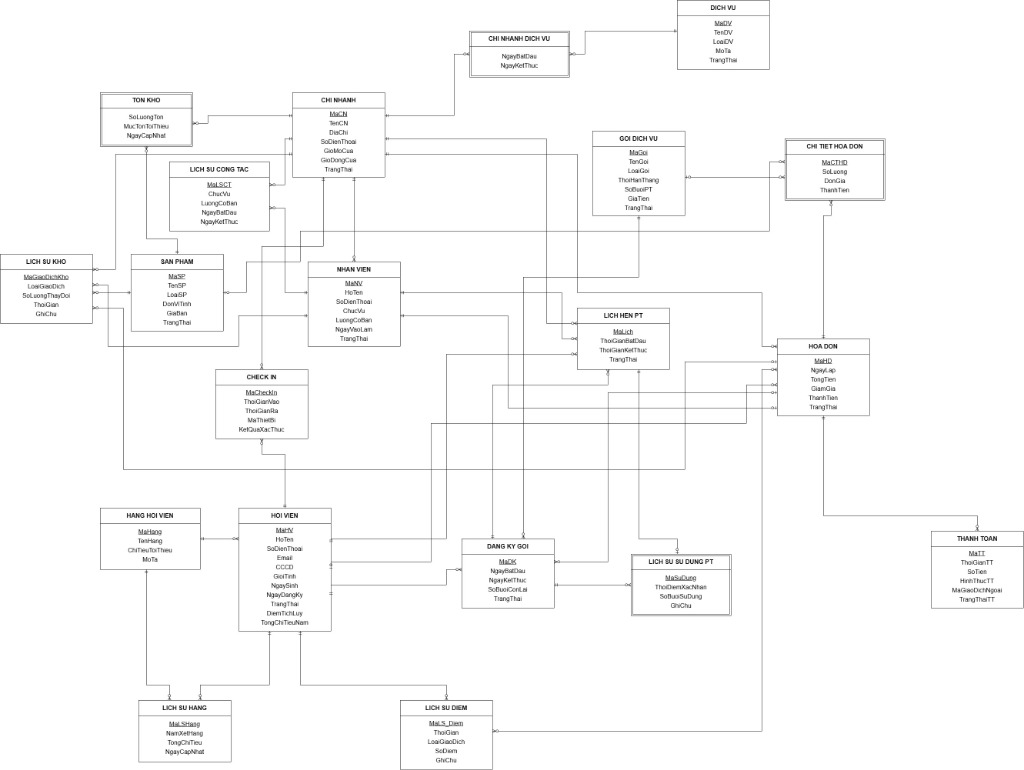
\includegraphics[width=\textwidth]{ER.jpg}
    \\[6pt]
    \textit{Hình 3.1: Mô hình thực thể kết hợp (ERD) hệ thống FitLife Hub}
\end{center}
\vspace{1em}

\subsection{Mô tả các ràng buộc nghiệp vụ (Business Rules)}
Phần này đặc tả chi tiết các quy tắc nghiệp vụ và điều kiện ràng buộc dữ liệu của hệ thống (bao gồm cả các điều kiện chưa thể hiện trực tiếp trên mô hình ERD).

\subsubsection{Chi nhánh}
\begin{itemize}
    \item \textbf{BR01.} Mỗi chi nhánh có một mã chi nhánh duy nhất.
    \item \textbf{BR02.} Thông tin của mỗi chi nhánh gồm tên chi nhánh, địa chỉ, số điện thoại, giờ mở cửa, giờ đóng cửa và trạng thái hoạt động.
    \item \textbf{BR03.} Mỗi chi nhánh có thể cung cấp nhiều dịch vụ và tiện ích như Gym, Yoga, GroupX, PT cá nhân và Spa/Sauna.
    \item \textbf{BR04.} Mỗi chi nhánh có thể kinh doanh nhiều sản phẩm bán lẻ và theo dõi số lượng tồn kho riêng của từng sản phẩm.
    \item \textbf{BR05.} Mỗi chi nhánh có thể có nhiều nhân viên làm việc tại cùng một thời điểm.
    \item \textbf{BR06.} Mỗi chi nhánh có thể tiếp nhận nhiều lượt check-in của hội viên.
    \item \textbf{BR07.} Mỗi chi nhánh có thể tổ chức nhiều lịch hẹn PT.
    \item \textbf{BR08.} Mỗi chi nhánh có thể phát sinh nhiều hóa đơn.
    \item \textbf{BR09.} Một chi nhánh có thể xuất hiện trong nhiều giai đoạn công tác của nhân viên; lịch sử các giai đoạn này giúp xác định nơi chuyển đi và nơi chuyển đến khi điều chuyển.
\end{itemize}

\subsubsection{Hội viên}
\begin{itemize}
    \item \textbf{BR10.} Mỗi hội viên có một mã hội viên duy nhất.
    \item \textbf{BR11.} Thông tin hội viên gồm họ tên, số điện thoại, email, CCCD, giới tính, ngày sinh, ngày đăng ký, trạng thái, điểm tích lũy hiện tại, tổng chi tiêu tích lũy trong năm và hạng thành viên hiện tại; CCCD không được trùng nhau.
    \item \textbf{BR12.} Một hội viên có thể đăng ký nhiều gói dịch vụ trong quá trình sử dụng.
    \item \textbf{BR13.} Một hội viên có thể thực hiện nhiều lượt check-in tại các chi nhánh.
    \item \textbf{BR14.} Một hội viên có thể đặt nhiều lịch hẹn PT.
    \item \textbf{BR15.} Một hội viên có thể có nhiều hóa đơn; riêng hóa đơn bán lẻ có thể không gắn với hội viên nào.
    \item \textbf{BR16.} Tại một thời điểm, mỗi hội viên chỉ có một hạng thành viên đang áp dụng được lưu trực tiếp trên hồ sơ hội viên để tra cứu nhanh; kết quả xếp hạng qua các năm được lưu vết tại lịch sử xét hạng.
    \item \textbf{BR17.} Hội viên có thể tích lũy hoặc bị điều chỉnh điểm Loyalty theo các giao dịch và quy định của chương trình.
\end{itemize}

\subsubsection{Gói dịch vụ}
\begin{itemize}
    \item \textbf{BR18.} Mỗi gói dịch vụ có một mã gói duy nhất.
    \item \textbf{BR19.} Thông tin của mỗi gói gồm tên gói, loại gói, thời hạn theo tháng nếu có, số buổi PT nếu có, giá tiền và trạng thái kinh doanh.
    \item \textbf{BR20.} Một gói dịch vụ có thể được nhiều hội viên đăng ký và một hội viên có thể đăng ký lại cùng gói nhiều lần.
    \item \textbf{BR21.} Một gói dịch vụ có thể xuất hiện trong nhiều dòng chi tiết hóa đơn khác nhau.
\end{itemize}

\subsubsection{Sản phẩm bán lẻ}
\begin{itemize}
    \item \textbf{BR22.} Mỗi sản phẩm bán lẻ có một mã sản phẩm duy nhất.
    \item \textbf{BR23.} Thông tin sản phẩm gồm tên sản phẩm, loại sản phẩm, đơn vị tính, giá bán và trạng thái kinh doanh.
    \item \textbf{BR24.} Một sản phẩm có thể được kinh doanh tại nhiều chi nhánh, nhưng số lượng tồn kho được quản lý riêng cho từng chi nhánh.
    \item \textbf{BR25.} Một sản phẩm có thể xuất hiện trong nhiều dòng chi tiết hóa đơn khác nhau.
\end{itemize}

\subsubsection{Đăng ký gói dịch vụ}
\begin{itemize}
    \item \textbf{BR26.} Mỗi lần đăng ký gói có một mã đăng ký riêng và thuộc về đúng một hội viên.
    \item \textbf{BR27.} Mỗi lần đăng ký tương ứng với đúng một gói dịch vụ.
    \item \textbf{BR28.} Mỗi lần đăng ký ghi nhận ngày bắt đầu, ngày kết thúc, trạng thái sử dụng, số buổi PT còn lại nếu có và hóa đơn mua gói nếu phát sinh; ngày kết thúc không được trước ngày bắt đầu.
\end{itemize}

\subsubsection{Check-in}
\begin{itemize}
    \item \textbf{BR29.} Mỗi lượt check-in có một mã check-in duy nhất.
    \item \textbf{BR30.} Mỗi lượt check-in gắn với đúng một hội viên.
    \item \textbf{BR31.} Mỗi lượt check-in diễn ra tại đúng một chi nhánh.
    \item \textbf{BR32.} Mỗi lượt check-in ghi nhận thời gian vào, thời gian ra nếu đã check-out, thiết bị kiểm soát nếu có và kết quả xác thực; thời gian ra không được trước thời gian vào.
    \item \textbf{BR33.} Hội viên chỉ được xác nhận vào tập khi gói sử dụng còn hiệu lực và phù hợp với dịch vụ, chi nhánh; lượt xác thực không hợp lệ phải được phân biệt với lượt vào tập thành công.
\end{itemize}

\subsubsection{Lịch hẹn PT}
\begin{itemize}
    \item \textbf{BR34.} Mỗi lịch hẹn PT có một mã lịch hẹn duy nhất.
    \item \textbf{BR35.} Mỗi lịch hẹn PT được đặt bởi đúng một hội viên.
    \item \textbf{BR36.} Mỗi lịch hẹn PT do đúng một nhân viên đảm nhiệm vai trò huấn luyện viên phụ trách.
    \item \textbf{BR37.} Mỗi lịch hẹn PT diễn ra tại đúng một chi nhánh.
    \item \textbf{BR38.} Mỗi lịch hẹn ghi nhận thời gian bắt đầu, thời gian kết thúc, gói PT được sử dụng và trạng thái Đã đặt, Đã hoàn thành hoặc Hủy; thời gian kết thúc phải sau thời gian bắt đầu.
    \item \textbf{BR39.} Hội viên phải có đăng ký gói PT hợp lệ, đặt lịch trước khi sử dụng dịch vụ PT và tổng số buổi đã đặt (chưa hủy) cùng số buổi đã sử dụng không được vượt quá số buổi của gói.
    \item \textbf{BR40.} Một huấn luyện viên không được nhận hai lịch hẹn còn hiệu lực bị trùng thời gian; đồng thời một hội viên cũng không được có hai lịch hẹn PT còn hiệu lực chồng lấn thời gian, kể cả khi có nhiều yêu cầu đặt lịch cùng lúc.
\end{itemize}

\subsubsection{Hóa đơn}
\begin{itemize}
    \item \textbf{BR41.} Mỗi hóa đơn có một mã hóa đơn duy nhất.
    \item \textbf{BR42.} Mỗi hóa đơn có thể gắn với một hội viên; giao dịch bán lẻ không có hội viên vẫn có thể lập hóa đơn.
    \item \textbf{BR43.} Mỗi hóa đơn do đúng một nhân viên lập.
    \item \textbf{BR44.} Mỗi hóa đơn phát sinh tại đúng một chi nhánh để theo dõi doanh thu.
    \item \textbf{BR45.} Một hóa đơn có thể gồm nhiều dòng mua gói dịch vụ hoặc sản phẩm; hóa đơn được xác nhận phải có ít nhất một dòng chi tiết.
    \item \textbf{BR46.} Mỗi hóa đơn ghi nhận ngày lập, tổng tiền, số tiền giảm giá, thành tiền phải trả và trạng thái; hình thức cùng kết quả thanh toán được ghi nhận riêng ở giao dịch thanh toán.
\end{itemize}

\subsubsection{Chi tiết hóa đơn}
\begin{itemize}
    \item \textbf{BR47.} Mỗi dòng chi tiết hóa đơn có một mã riêng và thuộc về đúng một hóa đơn.
    \item \textbf{BR48.} Mỗi dòng chi tiết ghi đúng một loại hàng được mua: hoặc một gói dịch vụ hoặc một sản phẩm bán lẻ, không đồng thời cả hai.
    \item \textbf{BR49.} Mỗi dòng chi tiết ghi nhận số lượng, đơn giá tại thời điểm bán và thành tiền của dòng đó; mức giảm giá chung được theo dõi tại hóa đơn.
\end{itemize}

\subsubsection{Hạng hội viên và Loyalty}
\begin{itemize}
    \item \textbf{BR50.} FitLife Hub có ba hạng hội viên là Silver, Gold và Platinum; mỗi hạng có mã hạng, tên hạng, ngưỡng chi tiêu tối thiểu và mô tả quyền lợi nếu có.
    \item \textbf{BR51.} Một hạng hội viên có thể được áp dụng cho nhiều hội viên trong cùng kỳ xét hạng.
    \item \textbf{BR52.} Cứ mỗi 100.000 VNĐ chi tiêu đủ điều kiện, hội viên được tích lũy một điểm Loyalty; cách xử lý phần chi tiêu lẻ được áp dụng theo chính sách của chương trình.
    \item \textbf{BR53.} Hạng hội viên được xét dựa trên tổng chi tiêu đủ điều kiện trong năm và ngưỡng quy định cho từng hạng.
\end{itemize}

\subsubsection{Nhân viên}
\begin{itemize}
    \item \textbf{BR54.} Mỗi nhân viên có một mã nhân viên duy nhất.
    \item \textbf{BR55.} Thông tin nhân viên gồm họ tên, số điện thoại, chức vụ, lương cơ bản, ngày vào làm và trạng thái làm việc.
    \item \textbf{BR56.} Mỗi nhân viên thuộc đúng một chi nhánh công tác hiện tại.
    \item \textbf{BR57.} Một nhân viên có thể lập nhiều hóa đơn.
    \item \textbf{BR58.} Một nhân viên đảm nhiệm vai trò huấn luyện viên có thể phụ trách nhiều lịch hẹn PT.
    \item \textbf{BR59.} Một nhân viên có thể được phân công hoặc điều chuyển qua nhiều chi nhánh trong thời gian làm việc.
\end{itemize}

\subsubsection{Lịch sử công tác nhân viên}
\begin{itemize}
    \item \textbf{BR60.} Mỗi giai đoạn công tác có một mã lịch sử riêng, xác định nhân viên, chi nhánh, chức vụ, lương cơ bản, ngày bắt đầu và ngày kết thúc nếu đã kết thúc; các khoảng công tác của cùng một nhân viên không được chồng lấn.
    \item \textbf{BR61.} Lịch sử công tác phải cho phép biết nhân viên làm việc tại chi nhánh nào vào một thời điểm trong quá khứ để tính đúng số buổi dạy, lương và hoa hồng theo chi nhánh.
\end{itemize}

\subsubsection{Dịch vụ}
\begin{itemize}
    \item \textbf{BR62.} Mỗi dịch vụ có một mã dịch vụ duy nhất.
    \item \textbf{BR63.} Thông tin của mỗi dịch vụ gồm tên dịch vụ, loại dịch vụ, mô tả nếu có và trạng thái cung cấp.
    \item \textbf{BR64.} Hệ thống quản lý riêng danh mục dịch vụ như Gym, Yoga, PT hoặc Spa với các gói dịch vụ được bán cho hội viên.
    \item \textbf{BR65.} Một dịch vụ có thể được nhiều chi nhánh cung cấp.
    \item \textbf{BR66.} Khi dịch vụ ngừng cung cấp, trạng thái của dịch vụ phải được cập nhật để phục vụ việc tra cứu và quản lý.
    \item \textbf{BR67.} Một chi nhánh chỉ được ghi nhận đang cung cấp dịch vụ khi có thông tin về việc cung cấp dịch vụ đó tại chi nhánh.
\end{itemize}

\subsubsection{Dịch vụ tại chi nhánh}
\begin{itemize}
    \item \textbf{BR68.} Mỗi bản ghi dịch vụ tại chi nhánh gắn với đúng một chi nhánh và một dịch vụ.
    \item \textbf{BR69.} Mỗi cặp chi nhánh và dịch vụ chỉ có một bản ghi trong danh sách dịch vụ của chi nhánh.
    \item \textbf{BR70.} Mỗi bản ghi ghi nhận ngày bắt đầu cung cấp và ngày kết thúc nếu dịch vụ đã ngừng.
    \item \textbf{BR71.} Ngày kết thúc cung cấp dịch vụ, nếu có, không được trước ngày bắt đầu.
    \item \textbf{BR72.} Một chi nhánh có thể cung cấp nhiều dịch vụ và một dịch vụ có thể có mặt tại nhiều chi nhánh.
\end{itemize}

\subsubsection{Tồn kho sản phẩm}
\begin{itemize}
    \item \textbf{BR73.} Mỗi bản ghi tồn kho thuộc về đúng một chi nhánh và đúng một sản phẩm.
    \item \textbf{BR74.} Tại một chi nhánh, mỗi sản phẩm chỉ có một bản ghi theo dõi số lượng tồn kho hiện tại.
    \item \textbf{BR75.} Mỗi bản ghi tồn kho ghi nhận số lượng còn lại, mức tồn tối thiểu và thời điểm cập nhật gần nhất.
    \item \textbf{BR76.} Số lượng tồn kho và mức tồn tối thiểu không được là số âm.
    \item \textbf{BR77.} Khi bán sản phẩm, hệ thống phải kiểm tra lượng tồn tại chính chi nhánh lập hóa đơn trước khi xác nhận giao dịch.
    \item \textbf{BR78.} Khi nhập, xuất hoặc điều chỉnh hàng, số lượng tồn kho được cập nhật và có thể tra cứu các sản phẩm xuống dưới mức tồn tối thiểu.
\end{itemize}

\subsubsection{Lịch sử biến động kho}
\begin{itemize}
    \item \textbf{BR79.} Mỗi giao dịch nhập, xuất hoặc điều chỉnh kho có một mã giao dịch kho duy nhất.
    \item \textbf{BR80.} Mỗi giao dịch kho thuộc về đúng một chi nhánh và một sản phẩm.
    \item \textbf{BR81.} Mỗi giao dịch kho do đúng một nhân viên thực hiện hoặc ghi nhận.
    \item \textbf{BR82.} Giao dịch kho có thể liên quan đến một hóa đơn; trường hợp nhập hàng hoặc điều chỉnh không cần gắn hóa đơn.
    \item \textbf{BR83.} Mỗi giao dịch ghi nhận loại giao dịch, số lượng thay đổi, thời điểm phát sinh và ghi chú lý do nếu có.
    \item \textbf{BR84.} Việc nhập, xuất và điều chỉnh kho phải làm thay đổi lượng tồn theo đúng quy ước và không được khiến tồn kho trở thành số âm.
    \item \textbf{BR85.} Lịch sử biến động kho phải được giữ lại để tra cứu nguyên nhân chênh lệch và đối chiếu với số lượng tồn thực tế.
\end{itemize}

\subsubsection{Lịch sử sử dụng buổi PT}
\begin{itemize}
    \item \textbf{BR86.} Mỗi lần xác nhận sử dụng buổi PT có một mã sử dụng duy nhất.
    \item \textbf{BR87.} Mỗi bản ghi sử dụng PT gắn với đúng một lịch hẹn PT và một lần đăng ký gói PT.
    \item \textbf{BR88.} Một lịch hẹn PT có thể chưa có bản ghi sử dụng, nhưng nếu đã xác nhận thì chỉ có tối đa một bản ghi sử dụng cho lịch đó.
    \item \textbf{BR89.} Mỗi bản ghi ghi nhận thời điểm xác nhận, số buổi đã sử dụng và ghi chú nếu có.
    \item \textbf{BR90.} Số buổi PT chỉ được trừ theo quy định khi buổi tập được xác nhận hoàn thành, không trừ ngay khi mới đặt lịch.
    \item \textbf{BR91.} Số buổi đã sử dụng phải hợp lệ và không được vượt quá số buổi còn lại của đăng ký gói.
\end{itemize}

\subsubsection{Thanh toán}
\begin{itemize}
    \item \textbf{BR92.} Mỗi giao dịch thanh toán có một mã thanh toán duy nhất.
    \item \textbf{BR93.} Mỗi giao dịch thanh toán thuộc về đúng một hóa đơn; một hóa đơn có thể có nhiều lần thanh toán hoặc thử thanh toán.
    \item \textbf{BR94.} Mỗi giao dịch ghi nhận thời gian, số tiền thanh toán, hình thức thanh toán và trạng thái giao dịch.
    \item \textbf{BR95.} Hình thức thanh toán gồm tiền mặt, VNPay hoặc thẻ.
    \item \textbf{BR96.} Mã giao dịch của hệ thống thanh toán bên ngoài được lưu khi có phát sinh.
    \item \textbf{BR97.} Khi thanh toán thành công, hệ thống mới xác nhận các quyền lợi mua gói, cập nhật tồn kho, ghi nhận lịch sử điểm và cập nhật trực tiếp điểm tích lũy, tổng chi tiêu năm cùng hạng hiện tại cho hội viên.
    \item \textbf{BR98.} Giao dịch thất bại hoặc bị hủy phải được ghi nhận đúng trạng thái và không làm phát sinh quyền lợi hay trừ tồn kho sai quy định.
\end{itemize}

\subsubsection{Lịch sử điểm Loyalty}
\begin{itemize}
    \item \textbf{BR99.} Mỗi lần biến động điểm (cộng hoặc trừ điểm) có một mã lịch sử điểm duy nhất.
    \item \textbf{BR100.} Mỗi lần biến động điểm thuộc về đúng một hội viên.
    \item \textbf{BR101.} Một lần biến động điểm có thể gắn với hóa đơn đã thanh toán hoặc phát sinh từ việc điều chỉnh điểm độc lập.
    \item \textbf{BR102.} Mỗi bản ghi lưu thời gian, loại giao dịch cộng hoặc trừ điểm, số điểm thay đổi và ghi chú nếu có.
    \item \textbf{BR103.} Điểm chỉ được cộng cho các khoản chi tiêu đủ điều kiện theo quy định của chương trình.
    \item \textbf{BR104.} Lịch sử cộng, trừ điểm phải được giữ lại để kiểm tra số điểm của hội viên và xử lý khiếu nại.
\end{itemize}

\subsubsection{Lịch sử hạng hội viên}
\begin{itemize}
    \item \textbf{BR105.} Mỗi lần ghi nhận kết quả xét hạng có một mã lịch sử hạng duy nhất.
    \item \textbf{BR106.} Mỗi bản ghi xét hạng thuộc về đúng một hội viên và một hạng thành viên.
    \item \textbf{BR107.} Mỗi bản ghi lưu năm xét hạng, tổng chi tiêu trong kỳ và ngày cập nhật kết quả.
    \item \textbf{BR108.} Hạng hội viên được xác định dựa trên tổng chi tiêu hợp lệ của năm xét hạng và ngưỡng của từng hạng.
    \item \textbf{BR109.} Hội viên có thể được xét hạng qua nhiều năm; thông tin các lần xét hạng phải được lưu lại.
    \item \textbf{BR110.} Lịch sử hạng phải giúp lưu trữ kết quả xếp hạng của từng năm và đối chiếu việc nâng hoặc hạ hạng của hội viên theo thời gian.
\end{itemize}

\newpage

\section{Thiết kế mức logic}

\subsection{Lược đồ cơ sở dữ liệu quan hệ}
\textbf{Quy ước:} \pk{Khóa chính} được gạch liền dưới chân; \fk{khóa ngoại} được gạch đứt dưới chân; thuộc tính \pkfk{vừa là khóa chính vừa là khóa ngoại} được gạch cả nét liền và nét đứt; khóa ngoại cho phép NULL có thêm dấu \texttt{?} phía sau.

\begin{enumerate}[itemsep=4pt]
    \item \textbf{HANG\_HOI\_VIEN}(\pk{MaHang}, TenHang, ChiTieuToiThieu, MoTa)
    \item \textbf{HOI\_VIEN}(\pk{MaHV}, HoTen, SoDienThoai, Email, CCCD, GioiTinh, NgaySinh, NgayDangKy, TrangThai, DiemTichLuy, TongChiTieuNam, \fk{MaHang}) \\
    \hspace*{1em}\small\texttt{MaHang} $\rightarrow$ \texttt{HANG\_HOI\_VIEN(MaHang)}\normalsize
    \item \textbf{CHI\_NHANH}(\pk{MaCN}, TenCN, DiaChi, SoDienThoai, GioMoCua, GioDongCua, TrangThai)
    \item \textbf{NHAN\_VIEN}(\pk{MaNV}, HoTen, SoDienThoai, ChucVu, LuongCoBan, NgayVaoLam, TrangThai, \fk{MaCNHienTai}) \\
    \hspace*{1em}\small\texttt{MaCNHienTai} $\rightarrow$ \texttt{CHI\_NHANH(MaCN)}\normalsize
    \item \textbf{LICH\_SU\_CONG\_TAC}(\pk{MaLSCT}, ChucVu, LuongCoBan, NgayBatDau, NgayKetThuc, \fk{MaNV}, \fk{MaCN}) \\
    \hspace*{1em}\small\texttt{MaNV} $\rightarrow$ \texttt{NHAN\_VIEN(MaNV)}; \quad \texttt{MaCN} $\rightarrow$ \texttt{CHI\_NHANH(MaCN)}\normalsize
    \item \textbf{DICH\_VU}(\pk{MaDV}, TenDV, LoaiDV, MoTa, TrangThai)
    \item \textbf{CHI\_NHANH\_DICH\_VU}(\pkfk{MaCN}, \pkfk{MaDV}, NgayBatDau, NgayKetThuc) \\
    \hspace*{1em}\small\texttt{MaCN} $\rightarrow$ \texttt{CHI\_NHANH(MaCN)}; \quad \texttt{MaDV} $\rightarrow$ \texttt{DICH\_VU(MaDV)}\normalsize
    \item \textbf{GOI\_DICH\_VU}(\pk{MaGoi}, TenGoi, LoaiGoi, ThoiHanThang, SoBuoiPT, GiaTien, TrangThai)
    \item \textbf{SAN\_PHAM}(\pk{MaSP}, TenSP, LoaiSP, DonViTinh, GiaBan, TrangThai)
    \item \textbf{TON\_KHO}(\pkfk{MaCN}, \pkfk{MaSP}, SoLuongTon, MucTonToiThieu, NgayCapNhat) \\
    \hspace*{1em}\small\texttt{MaCN} $\rightarrow$ \texttt{CHI\_NHANH(MaCN)}; \quad \texttt{MaSP} $\rightarrow$ \texttt{SAN\_PHAM(MaSP)}\normalsize
    \item \textbf{LICH\_SU\_KHO}(\pk{MaGiaoDichKho}, LoaiGiaoDich, SoLuongThayDoi, ThoiGian, GhiChu, \fk{MaCN}, \fk{MaSP}, \fk{MaNV}, \fk{MaHD}?) \\
    \hspace*{1em}\small\texttt{MaCN} $\rightarrow$ \texttt{CHI\_NHANH(MaCN)}; \quad \texttt{MaSP} $\rightarrow$ \texttt{SAN\_PHAM(MaSP)}; \quad \texttt{MaNV} $\rightarrow$ \texttt{NHAN\_VIEN(MaNV)}; \quad \texttt{MaHD} $\rightarrow$ \texttt{HOA\_DON(MaHD)}\normalsize
    \item \textbf{HOA\_DON}(\pk{MaHD}, NgayLap, TongTien, GiamGia, ThanhTien, TrangThai, \fk{MaCN}, \fk{MaNV}, \fk{MaHV}?) \\
    \hspace*{1em}\small\texttt{MaCN} $\rightarrow$ \texttt{CHI\_NHANH(MaCN)}; \quad \texttt{MaNV} $\rightarrow$ \texttt{NHAN\_VIEN(MaNV)}; \quad \texttt{MaHV} $\rightarrow$ \texttt{HOI\_VIEN(MaHV)}\normalsize
    \item \textbf{CHI\_TIET\_HOA\_DON}(\pk{MaCTHD}, SoLuong, DonGia, ThanhTien, \fk{MaHD}, \fk{MaGoi}?, \fk{MaSP}?) \\
    \hspace*{1em}\small\texttt{MaHD} $\rightarrow$ \texttt{HOA\_DON(MaHD)}; \quad \texttt{MaGoi} $\rightarrow$ \texttt{GOI\_DICH\_VU(MaGoi)}; \quad \texttt{MaSP} $\rightarrow$ \texttt{SAN\_PHAM(MaSP)}\normalsize
    \item \textbf{THANH\_TOAN}(\pk{MaTT}, ThoiGianTT, SoTien, HinhThucTT, MaGiaoDichNgoai, TrangThaiTT, \fk{MaHD}) \\
    \hspace*{1em}\small\texttt{MaHD} $\rightarrow$ \texttt{HOA\_DON(MaHD)}\normalsize
    \item \textbf{DANG\_KY\_GOI}(\pk{MaDK}, NgayBatDau, NgayKetThuc, SoBuoiConLai, TrangThai, \fk{MaHV}, \fk{MaGoi}, \fk{MaHD}?) \\
    \hspace*{1em}\small\texttt{MaHV} $\rightarrow$ \texttt{HOI\_VIEN(MaHV)}; \quad \texttt{MaGoi} $\rightarrow$ \texttt{GOI\_DICH\_VU(MaGoi)}; \quad \texttt{MaHD} $\rightarrow$ \texttt{HOA\_DON(MaHD)}\normalsize
    \item \textbf{LICH\_HEN\_PT}(\pk{MaLich}, ThoiGianBatDau, ThoiGianKetThuc, TrangThai, \fk{MaHV}, \fk{MaNV}, \fk{MaCN}, \fk{MaDK}) \\
    \hspace*{1em}\small\texttt{MaHV} $\rightarrow$ \texttt{HOI\_VIEN(MaHV)}; \quad \texttt{MaNV} $\rightarrow$ \texttt{NHAN\_VIEN(MaNV)}; \quad \texttt{MaCN} $\rightarrow$ \texttt{CHI\_NHANH(MaCN)}; \quad \texttt{MaDK} $\rightarrow$ \texttt{DANG\_KY\_GOI(MaDK)}\normalsize
    \item \textbf{LICH\_SU\_SU\_DUNG\_PT}(\pk{MaSuDung}, ThoiDiemXacNhan, SoBuoiSuDung, GhiChu, \fk{MaLich}, \fk{MaDK}) \\
    \hspace*{1em}\small\texttt{MaLich} $\rightarrow$ \texttt{LICH\_HEN\_PT(MaLich)}; \quad \texttt{MaDK} $\rightarrow$ \texttt{DANG\_KY\_GOI(MaDK)}\normalsize
    \item \textbf{CHECK\_IN}(\pk{MaCheckIn}, ThoiGianVao, ThoiGianRa, MaThietBi, KetQuaXacThuc, \fk{MaHV}, \fk{MaCN}) \\
    \hspace*{1em}\small\texttt{MaHV} $\rightarrow$ \texttt{HOI\_VIEN(MaHV)}; \quad \texttt{MaCN} $\rightarrow$ \texttt{CHI\_NHANH(MaCN)}\normalsize
    \item \textbf{LICH\_SU\_DIEM}(\pk{MaLS\_Diem}, ThoiGian, LoaiGiaoDich, SoDiem, GhiChu, \fk{MaHV}, \fk{MaHD}?) \\
    \hspace*{1em}\small\texttt{MaHV} $\rightarrow$ \texttt{HOI\_VIEN(MaHV)}; \quad \texttt{MaHD} $\rightarrow$ \texttt{HOA\_DON(MaHD)}\normalsize
    \item \textbf{LICH\_SU\_HANG}(\pk{MaLSHang}, NamXetHang, TongChiTieu, NgayCapNhat, \fk{MaHV}, \fk{MaHang}) \\
    \hspace*{1em}\small\texttt{MaHV} $\rightarrow$ \texttt{HOI\_VIEN(MaHV)}; \quad \texttt{MaHang} $\rightarrow$ \texttt{HANG\_HOI\_VIEN(MaHang)}\normalsize
\end{enumerate}

\subsection{Xác định khóa, tập phụ thuộc hàm và dạng chuẩn của các quan hệ}

\subsubsection{Cơ sở phân tích}
\textbf{Ký hiệu:} \texttt{X $\rightarrow$ Y} đọc là ``X xác định hàm Y''. Siêu khóa là tập thuộc tính có bao đóng bằng toàn bộ quan hệ; khóa dự tuyển là siêu khóa tối thiểu; thuộc tính khóa là thuộc tính nằm trong ít nhất một khóa dự tuyển.

\textbf{Tiêu chí xét dạng chuẩn:}

\vspace{0.5em}
\begin{small}
\begin{tabularx}{\textwidth}{| C{2.6cm} | Y |}
\hline
\textbf{Dạng chuẩn} & \textbf{Điều kiện} \\
\hline
1NF & Mọi thuộc tính nguyên tử, không có thuộc tính đa trị hay nhóm lặp (HoTen, DiaChi được xem là một giá trị nguyên tử trong miền bài toán). \\
\hline
2NF & Đạt 1NF và không có thuộc tính không khóa phụ thuộc vào một phần của khóa dự tuyển (chỉ cần xét khi khóa gồm nhiều thuộc tính). \\
\hline
3NF & Đạt 2NF và với mọi phụ thuộc hàm không tầm thường \texttt{X $\rightarrow$ A}: X là siêu khóa hoặc A là thuộc tính khóa (không có phụ thuộc bắc cầu). \\
\hline
BCNF & Với mọi phụ thuộc hàm không tầm thường \texttt{X $\rightarrow$ A}: X là siêu khóa. \\
\hline
\end{tabularx}
\end{small}

\vspace{0.5em}
\textbf{Cách chọn khóa chính:} (1) liệt kê các phụ thuộc hàm của quan hệ; (2) tính bao đóng để tìm các khóa dự tuyển; (3) chọn làm khóa chính khóa dự tuyển gọn, ổn định (mã định danh sinh ra khi tạo bản ghi), thuận tiện để các quan hệ khác tham chiếu.

\textbf{Giả định về phụ thuộc hàm} (theo mô tả nghiệp vụ trong đề bài):
\begin{itemize}
    \item Chỉ những thuộc tính được khai báo UNIQUE trong đề bài mới là khóa dự tuyển bổ sung: \texttt{CCCD} (HOI\_VIEN), \texttt{TenHang} (HANG\_HOI\_VIEN), \texttt{MaLich} (LICH\_SU\_SU\_DUNG\_PT), (\texttt{MaHV}, \texttt{NamXetHang}) (LICH\_SU\_HANG).
    \item \texttt{SoDienThoai}, \texttt{Email} của hội viên không duy nhất; \texttt{ChucVu} không xác định \texttt{LuongCoBan} (lương cơ bản đặt theo từng nhân viên / từng giai đoạn công tác); \texttt{MaThietBi} chỉ là nhãn thiết bị, không xác định chi nhánh.
    \item Phụ thuộc giữa các quan hệ khác nhau (ví dụ chi nhánh hiện tại của nhân viên trùng với dòng công tác mới nhất) là dư thừa có chủ đích để tra cứu nhanh; không tính là vi phạm dạng chuẩn của từng quan hệ.
\end{itemize}

\subsubsection{Phân tích từng quan hệ}

\textbf{1. HANG\_HOI\_VIEN(\pk{MaHang}, TenHang, ChiTieuToiThieu, MoTa)}
\begin{itemize}
    \item \textbf{Phụ thuộc hàm:}
    \begin{itemize}
        \item F1: \texttt{MaHang $\rightarrow$ TenHang, ChiTieuToiThieu, MoTa}
        \item F2: \texttt{TenHang $\rightarrow$ MaHang, ChiTieuToiThieu, MoTa} (vì \texttt{TenHang} là UNIQUE)
    \end{itemize}
    \item \textbf{Khóa dự tuyển:} \texttt{MaHang}, \texttt{TenHang}.
    \item \textbf{Vì sao chọn \texttt{MaHang} làm khóa chính:} bao đóng \texttt{MaHang$^+$} chứa toàn bộ thuộc tính và \texttt{MaHang} chỉ gồm một thuộc tính nên tối thiểu. \texttt{TenHang} (Silver, Gold, Platinum) cũng là khóa dự tuyển nhưng là tên hiển thị, có thể đổi; mã định danh ổn định hơn để làm khóa ngoại cho LICH\_SU\_HANG.
    \item \textbf{Dạng chuẩn: BCNF.} Thuộc tính nguyên tử (1NF); khóa đơn nên không có phụ thuộc riêng phần (2NF); mọi định thức (\texttt{MaHang}, \texttt{TenHang}) đều là siêu khóa (BCNF, kéo theo 3NF).
\end{itemize}

\textbf{2. HOI\_VIEN(\pk{MaHV}, HoTen, SoDienThoai, Email, CCCD, GioiTinh, NgaySinh, NgayDangKy, TrangThai, DiemTichLuy, TongChiTieuNam, \fk{MaHang})}
\begin{itemize}
    \item \textbf{Phụ thuộc hàm:}
    \begin{itemize}
        \item F1: \texttt{MaHV $\rightarrow$ HoTen, SoDienThoai, Email, CCCD, GioiTinh, NgaySinh, NgayDangKy, TrangThai, DiemTichLuy, TongChiTieuNam, MaHang}
        \item F2: \texttt{CCCD $\rightarrow$ MaHV, HoTen, SoDienThoai, Email, GioiTinh, NgaySinh, NgayDangKy, TrangThai, DiemTichLuy, TongChiTieuNam, MaHang} (vì \texttt{CCCD} là UNIQUE, NOT NULL)
        \item F3: \texttt{TongChiTieuNam $\rightarrow$ MaHang} (hạng hiện tại của hội viên được xác định theo tổng chi tiêu trong năm)
        \item Không có: \texttt{HoTen $\rightarrow$}, \texttt{SoDienThoai $\rightarrow$}, \texttt{Email $\rightarrow$} (trùng tên; số điện thoại và email không bắt buộc duy nhất).
    \end{itemize}
    \item \textbf{Khóa dự tuyển:} \texttt{MaHV}, \texttt{CCCD}.
    \item \textbf{Vì sao chọn \texttt{MaHV} làm khóa chính:} cả hai đều xác định toàn bộ thuộc tính. Hệ thống sinh \texttt{MaHV} khi đăng ký, nên giá trị này ổn định. Các hóa đơn, lịch hẹn, lịch sử check-in phải vẫn liên kết đúng khi thông tin cá nhân được chỉnh sửa. \texttt{CCCD} là dữ liệu cá nhân nhạy cảm, có thể nhập sai hoặc cập nhật, nên không dùng làm khóa ngoại ở nhiều bảng. \texttt{CCCD} được giữ lại với ràng buộc UNIQUE.
    \item \textbf{Dạng chuẩn: 2NF (không đạt 3NF).} Khóa đơn nên đạt 2NF. Tuy nhiên ở F3, định thức \texttt{TongChiTieuNam} không phải siêu khóa và \texttt{MaHang} không phải thuộc tính khóa, nên tồn tại phụ thuộc bắc cầu \texttt{MaHV $\rightarrow$ TongChiTieuNam $\rightarrow$ MaHang}.
    \item \textbf{Lý do giữ nguyên:} \texttt{DiemTichLuy}, \texttt{TongChiTieuNam} và \texttt{MaHang} là các thuộc tính tổng hợp/dẫn xuất được lưu trực tiếp trên hồ sơ hội viên nhằm giải quyết Vấn đề 4 của đề bài: loại bỏ việc tính lại toàn bộ hóa đơn 12 tháng mỗi khi thanh toán để in hóa đơn tức thì ($O(1)$), đồng thời được đồng bộ bằng Trigger.
\end{itemize}

\textbf{3. CHI\_NHANH(\pk{MaCN}, TenCN, DiaChi, SoDienThoai, GioMoCua, GioDongCua, TrangThai)}
\begin{itemize}
    \item \textbf{Phụ thuộc hàm:}
    \begin{itemize}
        \item F1: \texttt{MaCN $\rightarrow$ TenCN, DiaChi, SoDienThoai, GioMoCua, GioDongCua, TrangThai}
        \item Không có: \texttt{TenCN $\rightarrow$}, \texttt{DiaChi $\rightarrow$} (đề bài không khai báo UNIQUE); \texttt{GioMoCua}, \texttt{GioDongCua} độc lập với nhau.
    \end{itemize}
    \item \textbf{Khóa dự tuyển:} \texttt{MaCN}.
    \item \textbf{Vì sao chọn \texttt{MaCN}:} mã chi nhánh được đề bài quy định là định danh duy nhất của mỗi chi nhánh; \texttt{MaCN$^+$} là toàn bộ quan hệ và \texttt{MaCN} là khóa duy nhất.
    \item \textbf{Dạng chuẩn: BCNF.} Chỉ có một định thức là \texttt{MaCN}, là siêu khóa.
\end{itemize}

\textbf{4. NHAN\_VIEN(\pk{MaNV}, HoTen, SoDienThoai, ChucVu, LuongCoBan, NgayVaoLam, TrangThai, \fk{MaCNHienTai})}
\begin{itemize}
    \item \textbf{Phụ thuộc hàm:}
    \begin{itemize}
        \item F1: \texttt{MaNV $\rightarrow$ HoTen, SoDienThoai, ChucVu, LuongCoBan, NgayVaoLam, TrangThai, MaCNHienTai}
        \item Không có: \texttt{ChucVu $\rightarrow$ LuongCoBan} (lương đặt theo từng nhân viên), \texttt{MaCNHienTai $\rightarrow$ ChucVu}.
    \end{itemize}
    \item \textbf{Khóa dự tuyển:} \texttt{MaNV}.
    \item \textbf{Vì sao chọn \texttt{MaNV}:} họ tên và số điện thoại không đảm bảo duy nhất; chỉ mã nhân viên xác định được một nhân viên. \texttt{MaNV$^+$} là toàn bộ quan hệ.
    \item \textbf{Dạng chuẩn: BCNF.} Chỉ có định thức \texttt{MaNV}, là siêu khóa.
    \item \textbf{Lưu ý:} \texttt{ChucVu}, \texttt{LuongCoBan}, \texttt{MaCNHienTai} lặp lại thông tin của giai đoạn công tác hiện tại trong LICH\_SU\_CONG\_TAC để tra cứu nhanh. Đây là dư thừa giữa hai quan hệ; khi điều chuyển phải cập nhật đồng thời hai nơi.
\end{itemize}

\textbf{5. LICH\_SU\_CONG\_TAC(\pk{MaLSCT}, ChucVu, LuongCoBan, NgayBatDau, NgayKetThuc, \fk{MaNV}, \fk{MaCN})}
\begin{itemize}
    \item \textbf{Phụ thuộc hàm:}
    \begin{itemize}
        \item F1: \texttt{MaLSCT $\rightarrow$ MaNV, MaCN, ChucVu, LuongCoBan, NgayBatDau, NgayKetThuc}
        \item F2: \texttt{MaNV, NgayBatDau $\rightarrow$ MaLSCT, MaCN, ChucVu, LuongCoBan, NgayKetThuc} (các giai đoạn công tác của cùng một nhân viên không chồng lấn, nên một nhân viên chỉ bắt đầu một giai đoạn vào một ngày)
        \item Không có: \texttt{MaNV $\rightarrow$}, \texttt{MaCN $\rightarrow$}, \texttt{ChucVu $\rightarrow$ LuongCoBan} (một nhân viên có nhiều giai đoạn, mỗi giai đoạn chức vụ và lương riêng).
    \end{itemize}
    \item \textbf{Khóa dự tuyển:} \texttt{MaLSCT}; (\texttt{MaNV}, \texttt{NgayBatDau}).
    \item \textbf{Vì sao chọn \texttt{MaLSCT}:} khóa tự nhiên (\texttt{MaNV}, \texttt{NgayBatDau}) gồm hai thuộc tính và ngày bắt đầu có thể bị điều chỉnh. Mã bản ghi một thuộc tính ổn định và gọn hơn, nhưng cần ràng buộc UNIQUE (\texttt{MaNV}, \texttt{NgayBatDau}).
    \item \textbf{Dạng chuẩn: BCNF.} Với khóa dự tuyển (\texttt{MaNV}, \texttt{NgayBatDau}), không thuộc tính nào phụ thuộc riêng vào \texttt{MaNV} hoặc \texttt{NgayBatDau} (đạt 2NF); hai định thức \texttt{MaLSCT} và (\texttt{MaNV}, \texttt{NgayBatDau}) đều là siêu khóa.
\end{itemize}

\textbf{6. DICH\_VU(\pk{MaDV}, TenDV, LoaiDV, MoTa, TrangThai)}
\begin{itemize}
    \item \textbf{Phụ thuộc hàm:}
    \begin{itemize}
        \item F1: \texttt{MaDV $\rightarrow$ TenDV, LoaiDV, MoTa, TrangThai}
        \item Không có: \texttt{LoaiDV $\rightarrow$} (một loại như Gym, Yoga, PT, Spa gồm nhiều dịch vụ), \texttt{TenDV $\rightarrow$} (đề bài không khai báo UNIQUE).
    \end{itemize}
    \item \textbf{Khóa dự tuyển:} \texttt{MaDV}.
    \item \textbf{Vì sao chọn \texttt{MaDV}:} mã dịch vụ là định danh do hệ thống cấp; \texttt{MaDV$^+$} là toàn bộ quan hệ. Tên và loại dịch vụ không đủ để phân biệt các dịch vụ.
    \item \textbf{Dạng chuẩn: BCNF.} Chỉ có định thức \texttt{MaDV}, là siêu khóa.
\end{itemize}

\textbf{7. CHI\_NHANH\_DICH\_VU(\pkfk{MaCN}, \pkfk{MaDV}, NgayBatDau, NgayKetThuc)}
\begin{itemize}
    \item \textbf{Phụ thuộc hàm:}
    \begin{itemize}
        \item F1: \texttt{MaCN, MaDV $\rightarrow$ NgayBatDau, NgayKetThuc}
        \item Không có: \texttt{MaCN $\rightarrow$ NgayBatDau}, \texttt{MaDV $\rightarrow$ NgayBatDau} (ngày bắt đầu cung cấp là của từng cặp chi nhánh -- dịch vụ).
    \end{itemize}
    \item \textbf{Khóa dự tuyển:} (\texttt{MaCN}, \texttt{MaDV}).
    \item \textbf{Vì sao khóa chính là khóa ghép (\texttt{MaCN}, \texttt{MaDV}):} quan hệ này giải quyết liên kết nhiều--nhiều giữa chi nhánh và dịch vụ. Từng thuộc tính riêng lẻ không xác định được \texttt{NgayBatDau}/\texttt{NgayKetThuc}; chỉ cặp (\texttt{MaCN}, \texttt{MaDV}) mới xác định, và mỗi cặp xuất hiện một lần.
    \item \textbf{Dạng chuẩn: BCNF.} Không có phụ thuộc riêng phần vào \texttt{MaCN} hoặc \texttt{MaDV} (2NF); định thức duy nhất là khóa.
    \item \textbf{Lưu ý:} với khóa này mỗi cặp chi nhánh -- dịch vụ chỉ lưu được một giai đoạn cung cấp. Nếu cần ghi nhận dịch vụ ngừng rồi cung cấp lại, phải thêm \texttt{NgayBatDau} vào khóa.
\end{itemize}

\textbf{8. GOI\_DICH\_VU(\pk{MaGoi}, TenGoi, LoaiGoi, ThoiHanThang, SoBuoiPT, GiaTien, TrangThai)}
\begin{itemize}
    \item \textbf{Phụ thuộc hàm:}
    \begin{itemize}
        \item F1: \texttt{MaGoi $\rightarrow$ TenGoi, LoaiGoi, ThoiHanThang, SoBuoiPT, GiaTien, TrangThai}
        \item Không có: \texttt{LoaiGoi $\rightarrow$ ThoiHanThang, SoBuoiPT, GiaTien} (cùng loại gói có thể khác thời hạn, số buổi, giá), \texttt{TenGoi $\rightarrow$} (không khai báo UNIQUE).
    \end{itemize}
    \item \textbf{Khóa dự tuyển:} \texttt{MaGoi}.
    \item \textbf{Vì sao chọn \texttt{MaGoi}:} là mã định danh của gói; \texttt{MaGoi$^+$} là toàn bộ quan hệ. Các thuộc tính còn lại đều có thể trùng giữa các gói.
    \item \textbf{Dạng chuẩn: BCNF.} Chỉ có định thức \texttt{MaGoi}, là siêu khóa. Việc \texttt{ThoiHanThang}, \texttt{SoBuoiPT} có thể NULL (``nếu áp dụng'') không ảnh hưởng dạng chuẩn.
\end{itemize}

\textbf{9. SAN\_PHAM(\pk{MaSP}, TenSP, LoaiSP, DonViTinh, GiaBan, TrangThai)}
\begin{itemize}
    \item \textbf{Phụ thuộc hàm:}
    \begin{itemize}
        \item F1: \texttt{MaSP $\rightarrow$ TenSP, LoaiSP, DonViTinh, GiaBan, TrangThai}
        \item Không có: \texttt{LoaiSP $\rightarrow$ DonViTinh} (đề bài không quy định mỗi loại có đơn vị tính cố định), \texttt{TenSP $\rightarrow$} (không khai báo UNIQUE).
    \end{itemize}
    \item \textbf{Khóa dự tuyển:} \texttt{MaSP}.
    \item \textbf{Vì sao chọn \texttt{MaSP}:} là mã định danh sản phẩm; \texttt{MaSP$^+$} là toàn bộ quan hệ.
    \item \textbf{Dạng chuẩn: BCNF.} Chỉ có định thức \texttt{MaSP}, là siêu khóa.
    \item \textbf{Lưu ý:} \texttt{GiaBan} là giá hiện tại; giá tại thời điểm bán được lưu riêng ở \texttt{CHI\_TIET\_HOA\_DON.DonGia}.
\end{itemize}

\textbf{10. TON\_KHO(\pkfk{MaCN}, \pkfk{MaSP}, SoLuongTon, MucTonToiThieu, NgayCapNhat)}
\begin{itemize}
    \item \textbf{Phụ thuộc hàm:}
    \begin{itemize}
        \item F1: \texttt{MaCN, MaSP $\rightarrow$ SoLuongTon, MucTonToiThieu, NgayCapNhat}
        \item Không có: \texttt{MaSP $\rightarrow$ SoLuongTon} (tồn kho phụ thuộc đồng thời vào sản phẩm và chi nhánh), \texttt{MaCN $\rightarrow$ SoLuongTon}.
    \end{itemize}
    \item \textbf{Khóa dự tuyển:} (\texttt{MaCN}, \texttt{MaSP}).
    \item \textbf{Vì sao khóa chính là khóa ghép (\texttt{MaCN}, \texttt{MaSP}):} mỗi chi nhánh có lượng tồn riêng cho từng sản phẩm; chỉ biết chi nhánh hoặc chỉ biết sản phẩm thì không xác định được số lượng tồn. Khóa ghép bảo đảm mỗi cặp chi nhánh -- sản phẩm chỉ có một dòng tồn kho.
    \item \textbf{Dạng chuẩn: BCNF.} Cả ba thuộc tính không khóa phụ thuộc vào toàn bộ khóa (2NF); định thức duy nhất là khóa.
    \item \textbf{Giả định:} \texttt{MucTonToiThieu} đặt riêng cho từng cặp chi nhánh -- sản phẩm. Nếu mọi chi nhánh dùng chung một ngưỡng cho mỗi sản phẩm thì thuộc tính này chỉ phụ thuộc \texttt{MaSP} (vi phạm 2NF) và phải chuyển sang SAN\_PHAM.
\end{itemize}

\textbf{11. LICH\_SU\_KHO(\pk{MaGiaoDichKho}, LoaiGiaoDich, SoLuongThayDoi, ThoiGian, GhiChu, \fk{MaCN}, \fk{MaSP}, \fk{MaNV}, \fk{MaHD}?)}
\begin{itemize}
    \item \textbf{Phụ thuộc hàm:}
    \begin{itemize}
        \item F1: \texttt{MaGiaoDichKho $\rightarrow$ LoaiGiaoDich, SoLuongThayDoi, ThoiGian, GhiChu, MaCN, MaSP, MaNV, MaHD}
        \item Không có: \texttt{LoaiGiaoDich $\rightarrow$ SoLuongThayDoi} (cùng loại giao dịch có số lượng khác nhau), (\texttt{MaCN}, \texttt{MaSP}) $\rightarrow$ thuộc tính nào khác (một cặp chi nhánh -- sản phẩm có nhiều giao dịch kho).
    \end{itemize}
    \item \textbf{Khóa dự tuyển:} \texttt{MaGiaoDichKho}.
    \item \textbf{Vì sao chọn \texttt{MaGiaoDichKho}:} mỗi lần nhập, xuất hoặc điều chỉnh là một sự kiện riêng; cùng chi nhánh, sản phẩm, nhân viên, thời điểm vẫn có thể xảy ra nhiều lần. Chỉ mã giao dịch kho phân biệt được từng sự kiện.
    \item \textbf{Dạng chuẩn: BCNF.} Khóa đơn nên không có phụ thuộc riêng phần; định thức duy nhất là khóa.
\end{itemize}

\textbf{12. HOA\_DON(\pk{MaHD}, NgayLap, TongTien, GiamGia, ThanhTien, TrangThai, \fk{MaCN}, \fk{MaNV}, \fk{MaHV}?)}
\begin{itemize}
    \item \textbf{Phụ thuộc hàm:}
    \begin{itemize}
        \item F1: \texttt{MaHD $\rightarrow$ NgayLap, TongTien, GiamGia, ThanhTien, TrangThai, MaCN, MaNV, MaHV}
        \item F2: \texttt{TongTien, GiamGia $\rightarrow$ ThanhTien} (vì \texttt{ThanhTien = TongTien $-$ GiamGia})
        \item Không có: \texttt{MaHV $\rightarrow$}, \texttt{MaNV $\rightarrow$} (một hội viên hay một nhân viên có nhiều hóa đơn).
    \end{itemize}
    \item \textbf{Khóa dự tuyển:} \texttt{MaHD}.
    \item \textbf{Vì sao chọn \texttt{MaHD}:} mỗi hóa đơn là một giao dịch riêng; chi nhánh, nhân viên, hội viên, ngày lập đều có thể trùng giữa các hóa đơn. \texttt{MaHD$^+$} là toàn bộ quan hệ.
    \item \textbf{Dạng chuẩn: 2NF (không đạt 3NF).} Khóa đơn nên đạt 2NF. Tuy nhiên ở F2, định thức (\texttt{TongTien}, \texttt{GiamGia}) không phải siêu khóa và \texttt{ThanhTien} không phải thuộc tính khóa, nên có phụ thuộc bắc cầu \texttt{MaHD $\rightarrow$ (TongTien, GiamGia) $\rightarrow$ ThanhTien}.
    \item \textbf{Lý do giữ nguyên:} \texttt{ThanhTien} là thuộc tính dẫn xuất, được lưu để các báo cáo doanh thu (tần suất cao) và thanh toán không phải tính lại. Cần ràng buộc \texttt{ThanhTien = TongTien $-$ GiamGia} (CHECK hoặc trigger) để tránh lệch. \texttt{TongTien} cũng bằng tổng \texttt{ThanhTien} các dòng của CHI\_TIET\_HOA\_DON (dư thừa giữa hai quan hệ).
\end{itemize}

\textbf{13. CHI\_TIET\_HOA\_DON(\pk{MaCTHD}, SoLuong, DonGia, ThanhTien, \fk{MaHD}, \fk{MaGoi}?, \fk{MaSP}?)}
\begin{itemize}
    \item \textbf{Phụ thuộc hàm:}
    \begin{itemize}
        \item F1: \texttt{MaCTHD $\rightarrow$ SoLuong, DonGia, ThanhTien, MaHD, MaGoi, MaSP}
        \item F2: \texttt{SoLuong, DonGia $\rightarrow$ ThanhTien} (vì \texttt{ThanhTien = SoLuong $\times$ DonGia})
        \item Không có: \texttt{MaGoi $\rightarrow$ DonGia}, \texttt{MaSP $\rightarrow$ DonGia} (đơn giá lưu tại thời điểm bán, giá niêm yết đổi theo thời gian nên cùng một mặt hàng có thể có nhiều đơn giá).
    \end{itemize}
    \item \textbf{Khóa dự tuyển:} \texttt{MaCTHD}. Không chọn (\texttt{MaHD}, \texttt{MaGoi}) hay (\texttt{MaHD}, \texttt{MaSP}) làm khóa vì một hóa đơn có thể có hai dòng cho cùng một mặt hàng (ví dụ khác đơn giá hoặc khuyến mãi) và hai cột này có thể NULL.
    \item \textbf{Vì sao chọn \texttt{MaCTHD}:} mỗi dòng chi tiết cần một định danh riêng, không phụ thuộc vào cột có thể NULL.
    \item \textbf{Dạng chuẩn: 2NF (không đạt 3NF).} Khóa đơn nên đạt 2NF. Ở F2, định thức (\texttt{SoLuong}, \texttt{DonGia}) không phải siêu khóa và \texttt{ThanhTien} không phải thuộc tính khóa, nên có phụ thuộc bắc cầu \texttt{MaCTHD $\rightarrow$ (SoLuong, DonGia) $\rightarrow$ ThanhTien}.
    \item \textbf{Lý do giữ nguyên:} \texttt{ThanhTien} dẫn xuất được lưu sẵn để cộng thành \texttt{TongTien} của hóa đơn nhanh hơn; cần CHECK \texttt{ThanhTien = SoLuong $\times$ DonGia}.
\end{itemize}

\textbf{14. THANH\_TOAN(\pk{MaTT}, ThoiGianTT, SoTien, HinhThucTT, MaGiaoDichNgoai, TrangThaiTT, \fk{MaHD})}
\begin{itemize}
    \item \textbf{Phụ thuộc hàm:}
    \begin{itemize}
        \item F1: \texttt{MaTT $\rightarrow$ ThoiGianTT, SoTien, HinhThucTT, MaGiaoDichNgoai, TrangThaiTT, MaHD}
        \item Không có: \texttt{MaHD $\rightarrow$} (một hóa đơn có thể có nhiều lần thanh toán), \texttt{MaGiaoDichNgoai $\rightarrow$} (đề bài không khai báo UNIQUE; tiền mặt không có mã ngoài).
    \end{itemize}
    \item \textbf{Khóa dự tuyển:} \texttt{MaTT}.
    \item \textbf{Vì sao chọn \texttt{MaTT}:} mỗi giao dịch thanh toán là một sự kiện riêng và một hóa đơn có thể có nhiều giao dịch (thất bại rồi thành công, nhiều phương thức), nên \texttt{MaHD} không thể làm khóa.
    \item \textbf{Dạng chuẩn: BCNF.} Khóa đơn; định thức duy nhất là khóa.
\end{itemize}

\textbf{15. DANG\_KY\_GOI(\pk{MaDK}, NgayBatDau, NgayKetThuc, SoBuoiConLai, TrangThai, \fk{MaHV}, \fk{MaGoi}, \fk{MaHD}?)}
\begin{itemize}
    \item \textbf{Phụ thuộc hàm:}
    \begin{itemize}
        \item F1: \texttt{MaDK $\rightarrow$ NgayBatDau, NgayKetThuc, SoBuoiConLai, TrangThai, MaHV, MaGoi, MaHD}
        \item Không có: (\texttt{MaHV}, \texttt{MaGoi}) $\rightarrow$ thuộc tính nào khác (một hội viên có thể mua cùng một gói nhiều lần, mỗi lần là một đăng ký); (\texttt{NgayBatDau}, \texttt{MaGoi}) $\rightarrow$ \texttt{NgayKetThuc} (trạng thái ``tạm dừng'' có thể làm lùi ngày kết thúc nên ngày kết thúc không suy ra cố định từ thời hạn gói).
    \end{itemize}
    \item \textbf{Khóa dự tuyển:} \texttt{MaDK}.
    \item \textbf{Vì sao chọn \texttt{MaDK}:} đề bài yêu cầu lưu riêng từng lần mua để truy vết lịch sử, thời hạn và quyền lợi, nên cặp (\texttt{MaHV}, \texttt{MaGoi}) không đủ làm khóa.
    \item \textbf{Dạng chuẩn: BCNF.} Khóa đơn; định thức duy nhất là khóa.
    \item \textbf{Lưu ý:} \texttt{SoBuoiConLai} là số liệu tổng hợp (\texttt{SoBuoiPT} của gói trừ tổng \texttt{SoBuoiSuDung} trong LICH\_SU\_SU\_DUNG\_PT), lưu sẵn để kiểm tra quyền lợi nhanh. Đây là dư thừa giữa các quan hệ, cần cập nhật cùng lúc khi ghi nhận buổi PT.
\end{itemize}

\textbf{16. LICH\_HEN\_PT(\pk{MaLich}, ThoiGianBatDau, ThoiGianKetThuc, TrangThai, \fk{MaHV}, \fk{MaNV}, \fk{MaCN}, \fk{MaDK})}
\begin{itemize}
    \item \textbf{Phụ thuộc hàm:}
    \begin{itemize}
        \item F1: \texttt{MaLich $\rightarrow$ ThoiGianBatDau, ThoiGianKetThuc, TrangThai, MaHV, MaNV, MaCN, MaDK}
        \item F2: \texttt{MaDK $\rightarrow$ MaHV} (mỗi đăng ký gói thuộc đúng một hội viên, nên đăng ký xác định hội viên)
        \item Không có: (\texttt{MaNV}, \texttt{ThoiGianBatDau}) $\rightarrow$ thuộc tính khác (lịch đã hủy có thể trùng giờ với lịch còn hiệu lực; việc cấm trùng chỉ áp cho lịch còn hiệu lực nên là ràng buộc riêng, không phải khóa).
    \end{itemize}
    \item \textbf{Khóa dự tuyển:} \texttt{MaLich}.
    \item \textbf{Vì sao chọn \texttt{MaLich}:} một hội viên, huấn luyện viên hay đăng ký gói đều có nhiều lịch hẹn; giờ bắt đầu có thể trùng giữa các lịch đã hủy. Chỉ mã lịch hẹn phân biệt từng lịch.
    \item \textbf{Dạng chuẩn: 2NF (không đạt 3NF).} Khóa đơn nên đạt 2NF. Ở F2, \texttt{MaDK} không phải siêu khóa (một đăng ký có nhiều lịch hẹn) và \texttt{MaHV} không phải thuộc tính khóa, nên có phụ thuộc bắc cầu \texttt{MaLich $\rightarrow$ MaDK $\rightarrow$ MaHV}.
    \item \textbf{Lý do giữ nguyên:} \texttt{MaHV} được giữ lại (đề bài liệt kê \texttt{MaHV} là khóa ngoại của LICH\_HEN\_PT) để tra cứu lịch của hội viên mà không phải nối thêm DANG\_KY\_GOI. Cần ràng buộc để \texttt{MaHV} của lịch hẹn luôn trùng \texttt{MaHV} của đăng ký gói tương ứng.
\end{itemize}

\textbf{17. LICH\_SU\_SU\_DUNG\_PT(\pk{MaSuDung}, ThoiDiemXacNhan, SoBuoiSuDung, GhiChu, \fk{MaLich}, \fk{MaDK})}
\begin{itemize}
    \item \textbf{Phụ thuộc hàm:}
    \begin{itemize}
        \item F1: \texttt{MaSuDung $\rightarrow$ ThoiDiemXacNhan, SoBuoiSuDung, GhiChu, MaLich, MaDK}
        \item F2: \texttt{MaLich $\rightarrow$ MaSuDung, ThoiDiemXacNhan, SoBuoiSuDung, GhiChu, MaDK} (vì \texttt{MaLich} là UNIQUE: mỗi lịch hẹn chỉ có một lần ghi nhận hoàn thành)
        \item Không có: \texttt{MaDK $\rightarrow$} (một đăng ký gói PT có nhiều lần sử dụng).
    \end{itemize}
    \item \textbf{Khóa dự tuyển:} \texttt{MaSuDung}, \texttt{MaLich}.
    \item \textbf{Vì sao chọn \texttt{MaSuDung}:} cả hai đều xác định toàn bộ thuộc tính. \texttt{MaSuDung} là mã bản ghi riêng của quan hệ, ổn định, không phụ thuộc vào quy tắc ``một lịch một lần ghi nhận'' (có thể đổi nếu chính sách cho phép ghi nhận nhiều lần). \texttt{MaLich} giữ lại với ràng buộc UNIQUE.
    \item \textbf{Dạng chuẩn: BCNF.} Hai định thức \texttt{MaSuDung} và \texttt{MaLich} đều là siêu khóa.
    \item \textbf{Lưu ý:} \texttt{MaDK} cũng suy ra được từ LICH\_HEN\_PT qua \texttt{MaLich}; đây là dư thừa giữa hai quan hệ, cần bảo đảm giá trị trùng nhau.
\end{itemize}

\textbf{18. CHECK\_IN(\pk{MaCheckIn}, ThoiGianVao, ThoiGianRa, MaThietBi, KetQuaXacThuc, \fk{MaHV}, \fk{MaCN})}
\begin{itemize}
    \item \textbf{Phụ thuộc hàm:}
    \begin{itemize}
        \item F1: \texttt{MaCheckIn $\rightarrow$ ThoiGianVao, ThoiGianRa, MaThietBi, KetQuaXacThuc, MaHV, MaCN}
        \item Không có: \texttt{MaThietBi $\rightarrow$ MaCN} (mã thiết bị chỉ là nhãn, có thể NULL hoặc trùng giữa các chi nhánh); (\texttt{MaHV}, \texttt{MaCN}, \texttt{ThoiGianVao}) $\rightarrow$ thuộc tính khác (các lần quét bị từ chối cũng được ghi nhận và có thể lặp).
    \end{itemize}
    \item \textbf{Khóa dự tuyển:} \texttt{MaCheckIn}.
    \item \textbf{Vì sao chọn \texttt{MaCheckIn}:} mỗi lượt quét là một sự kiện; không tổ hợp thuộc tính tự nhiên nào bảo đảm duy nhất (một hội viên có thể quét nhiều lần trong cùng giây, kể cả lần bị từ chối). Mã lượt check-in một thuộc tính cũng gọn, phù hợp cho bảng tăng nhanh cần chỉ mục và phân vùng.
    \item \textbf{Dạng chuẩn: BCNF.} Khóa đơn; định thức duy nhất là khóa.
\end{itemize}

\textbf{19. LICH\_SU\_DIEM(\pk{MaLS\_Diem}, ThoiGian, LoaiGiaoDich, SoDiem, GhiChu, \fk{MaHV}, \fk{MaHD}?)}
\begin{itemize}
    \item \textbf{Phụ thuộc hàm:}
    \begin{itemize}
        \item F1: \texttt{MaLS\_Diem $\rightarrow$ ThoiGian, LoaiGiaoDich, SoDiem, GhiChu, MaHV, MaHD}
        \item Không có: \texttt{MaHD $\rightarrow$ SoDiem} (một hóa đơn có thể có nhiều lần cộng/trừ điểm, và \texttt{MaHD} có thể NULL); \texttt{LoaiGiaoDich $\rightarrow$ SoDiem}.
    \end{itemize}
    \item \textbf{Khóa dự tuyển:} \texttt{MaLS\_Diem}.
    \item \textbf{Vì sao chọn \texttt{MaLS\_Diem}:} mỗi lần cộng hoặc trừ điểm là một giao dịch riêng để truy vết và giải quyết khiếu nại; (\texttt{MaHV}, \texttt{MaHD}) không đủ vì \texttt{MaHD} có thể NULL và có thể có nhiều giao dịch cho cùng một hóa đơn.
    \item \textbf{Dạng chuẩn: BCNF.} Khóa đơn; định thức duy nhất là khóa.
    \item \textbf{Lưu ý:} quy tắc chống cộng điểm trùng khi thanh toán xử lý lặp là ràng buộc nghiệp vụ riêng, không phải phụ thuộc hàm.
\end{itemize}

\textbf{20. LICH\_SU\_HANG(\pk{MaLSHang}, NamXetHang, TongChiTieu, NgayCapNhat, \fk{MaHV}, \fk{MaHang})}
\begin{itemize}
    \item \textbf{Phụ thuộc hàm:}
    \begin{itemize}
        \item F1: \texttt{MaLSHang $\rightarrow$ NamXetHang, TongChiTieu, NgayCapNhat, MaHV, MaHang}
        \item F2: \texttt{MaHV, NamXetHang $\rightarrow$ MaLSHang, TongChiTieu, NgayCapNhat, MaHang} (mỗi hội viên chỉ có một kết quả hạng cuối cùng cho mỗi năm xét hạng)
        \item Không có: \texttt{TongChiTieu $\rightarrow$ MaHang}. Hạng được xác định theo ngưỡng \texttt{ChiTieuToiThieu}, nhưng ngưỡng do doanh nghiệp quy định và có thể thay đổi; hạng được lưu như một sự kiện lịch sử đã xác lập, không suy lại từ tổng chi tiêu.
    \end{itemize}
    \item \textbf{Khóa dự tuyển:} \texttt{MaLSHang}; (\texttt{MaHV}, \texttt{NamXetHang}).
    \item \textbf{Vì sao chọn \texttt{MaLSHang}:} quan hệ này giải quyết liên kết nhiều--nhiều giữa HOI\_VIEN và HANG\_HOI\_VIEN. Khóa tự nhiên (\texttt{MaHV}, \texttt{NamXetHang}) có hai thuộc tính và sẽ phải thay đổi nếu chính sách cần lưu nhiều lần thay đổi hạng trong một năm; mã bản ghi một thuộc tính linh hoạt hơn, kèm ràng buộc UNIQUE (\texttt{MaHV}, \texttt{NamXetHang}).
    \item \textbf{Dạng chuẩn: BCNF.} Không có thuộc tính nào phụ thuộc riêng vào \texttt{MaHV} hoặc \texttt{NamXetHang} (2NF); hai định thức \texttt{MaLSHang} và (\texttt{MaHV}, \texttt{NamXetHang}) đều là siêu khóa.
\end{itemize}

\subsubsection{Kết luận dạng chuẩn của lược đồ CSDL}

\vspace{0.5em}
\begin{small}
\begin{tabularx}{\textwidth}{| C{1.1cm} | Y | C{3.4cm} | C{3.8cm} | C{2.6cm} |}
\hline
\textbf{STT} & \textbf{Quan hệ} & \textbf{Khóa chính} & \textbf{Khóa dự tuyển khác} & \textbf{Dạng chuẩn đạt được} \\
\hline
1 & HANG\_HOI\_VIEN & MaHang & TenHang & BCNF \\
\hline
2 & HOI\_VIEN & MaHV & CCCD & \textbf{2NF} \\
\hline
3 & CHI\_NHANH & MaCN & --- & BCNF \\
\hline
4 & NHAN\_VIEN & MaNV & --- & BCNF \\
\hline
5 & LICH\_SU\_CONG\_TAC & MaLSCT & (MaNV, NgayBatDau) & BCNF \\
\hline
6 & DICH\_VU & MaDV & --- & BCNF \\
\hline
7 & CHI\_NHANH\_DICH\_VU & (MaCN, MaDV) & --- & BCNF \\
\hline
8 & GOI\_DICH\_VU & MaGoi & --- & BCNF \\
\hline
9 & SAN\_PHAM & MaSP & --- & BCNF \\
\hline
10 & TON\_KHO & (MaCN, MaSP) & --- & BCNF \\
\hline
11 & LICH\_SU\_KHO & MaGiaoDichKho & --- & BCNF \\
\hline
12 & HOA\_DON & MaHD & --- & \textbf{2NF} \\
\hline
13 & CHI\_TIET\_HOA\_DON & MaCTHD & --- & \textbf{2NF} \\
\hline
14 & THANH\_TOAN & MaTT & --- & BCNF \\
\hline
15 & DANG\_KY\_GOI & MaDK & --- & BCNF \\
\hline
16 & LICH\_HEN\_PT & MaLich & --- & \textbf{2NF} \\
\hline
17 & LICH\_SU\_SU\_DUNG\_PT & MaSuDung & MaLich & BCNF \\
\hline
18 & CHECK\_IN & MaCheckIn & --- & BCNF \\
\hline
19 & LICH\_SU\_DIEM & MaLS\_Diem & --- & BCNF \\
\hline
20 & LICH\_SU\_HANG & MaLSHang & (MaHV, NamXetHang) & BCNF \\
\hline
\end{tabularx}
\end{small}

\vspace{0.5em}
\textbf{Kết luận:} Lược đồ cơ sở dữ liệu đạt \textbf{dạng chuẩn 2NF}, vì dạng chuẩn của cả lược đồ được xác định bởi quan hệ có dạng chuẩn thấp nhất. Trong 20 quan hệ, 16 quan hệ đạt BCNF (kéo theo 3NF, 2NF và 1NF). Bốn quan hệ HOI\_VIEN, HOA\_DON, CHI\_TIET\_HOA\_DON và LICH\_HEN\_PT đạt 2NF nhưng không đạt 3NF do phụ thuộc bắc cầu:
\begin{itemize}
    \item \textbf{HOI\_VIEN:} \texttt{TongChiTieuNam $\rightarrow$ MaHang} (phụ thuộc bắc cầu \texttt{MaHV $\rightarrow$ TongChiTieuNam $\rightarrow$ MaHang}).
    \item \textbf{HOA\_DON:} \texttt{ThanhTien = TongTien $-$ GiamGia} (phụ thuộc bắc cầu).
    \item \textbf{CHI\_TIET\_HOA\_DON:} \texttt{ThanhTien = SoLuong $\times$ DonGia} (phụ thuộc bắc cầu).
    \item \textbf{LICH\_HEN\_PT:} \texttt{MaDK $\rightarrow$ MaHV} (phụ thuộc bắc cầu \texttt{MaLich $\rightarrow$ MaDK $\rightarrow$ MaHV}).
\end{itemize}
Cả bốn đều là dư thừa có chủ đích (Denormalization) nhằm tăng tốc thanh toán, báo cáo doanh thu và tra cứu tức thì; các thuộc tính này được bảo vệ bằng ràng buộc CHECK hoặc trigger để bảo đảm dữ liệu luôn nhất quán.

\vspace{0.5em}
\textbf{Ghi chú về khóa và ràng buộc tổng quát:}

\vspace{0.3em}
\begin{small}
\begin{tabularx}{\textwidth}{| C{5cm} | Y |}
\hline
\textbf{Quan hệ} & \textbf{Ghi chú} \\
\hline
CHI\_NHANH\_DICH\_VU, TON\_KHO & Khóa chính là khóa kép gồm 2 khóa ngoại (ERD không có thuộc tính khóa riêng). \\
\hline
HOI\_VIEN & \texttt{CCCD} UNIQUE, NOT NULL. \\
\hline
HANG\_HOI\_VIEN & \texttt{TenHang} UNIQUE. \\
\hline
LICH\_SU\_CONG\_TAC & UNIQUE (\texttt{MaNV}, \texttt{NgayBatDau}); các giai đoạn của cùng nhân viên không chồng lấn. \\
\hline
LICH\_SU\_SU\_DUNG\_PT & \texttt{MaLich} là UNIQUE (quan hệ 1--0..1 với LICH\_HEN\_PT). \\
\hline
LICH\_SU\_HANG & UNIQUE (\texttt{MaHV}, \texttt{NamXetHang}) nếu chỉ lưu kết quả cuối cùng của mỗi năm. \\
\hline
HOA\_DON.MaHV & NULL khi khách vãng lai không phải hội viên. \\
\hline
CHI\_TIET\_HOA\_DON & Mỗi dòng chỉ chứa một trong hai: \texttt{MaGoi} hoặc \texttt{MaSP} (CHECK: đúng một cột khác NULL). \\
\hline
DANG\_KY\_GOI.MaHD, LICH\_SU\_KHO.MaHD, LICH\_SU\_DIEM.MaHD & Cho phép NULL (phát sinh không từ hóa đơn: nhập kho, điều chỉnh điểm, đăng ký tặng...). \\
\hline
\end{tabularx}
\end{small}

\newpage

\subsection{Mô tả ràng buộc toàn vẹn: Bối cảnh -- Nội dung -- Bảng tầm ảnh hưởng}

\subsubsection{A. Ràng buộc liên bộ}

\textbf{RBTV01. CCCD hội viên duy nhất} \\
\textbf{Bối cảnh:} HOI\_VIEN \\
\textbf{Nội dung:} $\forall t_1, t_2 \in \text{HOI\_VIEN} \; (t_1 \neq t_2 \Rightarrow t_1.\text{CCCD} \neq t_2.\text{CCCD})$

\vspace{0.3em}
\begin{small}
\begin{tabularx}{\textwidth}{| C{4.2cm} | C{2cm} | C{2cm} | Y |}
\hline
\textbf{RBTV01} & \textbf{Thêm} & \textbf{Xóa} & \textbf{Sửa} \\
\hline
HOI\_VIEN & + & $-$ & +(CCCD) \\
\hline
\end{tabularx}
\end{small}

\vspace{0.8em}
\textbf{RBTV02. Tên hạng hội viên duy nhất} \\
\textbf{Bối cảnh:} HANG\_HOI\_VIEN \\
\textbf{Nội dung:} $\forall t_1, t_2 \in \text{HANG\_HOI\_VIEN} \; (t_1 \neq t_2 \Rightarrow t_1.\text{TenHang} \neq t_2.\text{TenHang})$

\vspace{0.3em}
\begin{small}
\begin{tabularx}{\textwidth}{| C{4.2cm} | C{2cm} | C{2cm} | Y |}
\hline
\textbf{RBTV02} & \textbf{Thêm} & \textbf{Xóa} & \textbf{Sửa} \\
\hline
HANG\_HOI\_VIEN & + & $-$ & +(TenHang) \\
\hline
\end{tabularx}
\end{small}

\vspace{0.8em}
\textbf{RBTV03. Mỗi lịch hẹn chỉ được ghi nhận sử dụng một lần} \\
\textbf{Bối cảnh:} LICH\_SU\_SU\_DUNG\_PT \\
\textbf{Nội dung:} $\forall t_1, t_2 \in \text{LICH\_SU\_SU\_DUNG\_PT} \; (t_1 \neq t_2 \Rightarrow t_1.\text{MaLich} \neq t_2.\text{MaLich})$

\vspace{0.3em}
\begin{small}
\begin{tabularx}{\textwidth}{| C{4.2cm} | C{2cm} | C{2cm} | Y |}
\hline
\textbf{RBTV03} & \textbf{Thêm} & \textbf{Xóa} & \textbf{Sửa} \\
\hline
LICH\_SU\_SU\_DUNG\_PT & + & $-$ & +(MaLich) \\
\hline
\end{tabularx}
\end{small}

\vspace{0.8em}
\textbf{RBTV04. Mỗi hội viên có một kết quả hạng cho mỗi năm xét hạng} \\
\textbf{Bối cảnh:} LICH\_SU\_HANG \\
\textbf{Nội dung:} $\forall t_1, t_2 \in \text{LICH\_SU\_HANG} \; (t_1 \neq t_2 \Rightarrow t_1.\text{MaHV} \neq t_2.\text{MaHV} \lor t_1.\text{NamXetHang} \neq t_2.\text{NamXetHang})$

\vspace{0.3em}
\begin{small}
\begin{tabularx}{\textwidth}{| C{4.2cm} | C{2cm} | C{2cm} | Y |}
\hline
\textbf{RBTV04} & \textbf{Thêm} & \textbf{Xóa} & \textbf{Sửa} \\
\hline
LICH\_SU\_HANG & + & $-$ & +(MaHV, NamXetHang) \\
\hline
\end{tabularx}
\end{small}

\vspace{0.8em}
\textbf{RBTV05. Mã giao dịch ngoài không bị ghi nhận lặp} \\
\textbf{Bối cảnh:} THANH\_TOAN \\
\textbf{Nội dung:} $\forall t_1, t_2 \in \text{THANH\_TOAN} \; (t_1 \neq t_2 \land t_1.\text{MaGiaoDichNgoai} \neq \text{NULL} \Rightarrow t_1.\text{MaGiaoDichNgoai} \neq t_2.\text{MaGiaoDichNgoai})$

\vspace{0.3em}
\begin{small}
\begin{tabularx}{\textwidth}{| C{4.2cm} | C{2cm} | C{2cm} | Y |}
\hline
\textbf{RBTV05} & \textbf{Thêm} & \textbf{Xóa} & \textbf{Sửa} \\
\hline
THANH\_TOAN & + & $-$ & +(MaGiaoDichNgoai) \\
\hline
\end{tabularx}
\end{small}

\vspace{0.8em}
\textbf{RBTV06. Mỗi hóa đơn chỉ được cộng điểm một lần} \\
\textbf{Bối cảnh:} LICH\_SU\_DIEM \\
\textbf{Nội dung:} $\forall t_1, t_2 \in \text{LICH\_SU\_DIEM} \; (t_1 \neq t_2 \land t_1.\text{LoaiGiaoDich} = \text{'Cộng'} \land t_1.\text{MaHD} \neq \text{NULL} \Rightarrow \neg(t_2.\text{LoaiGiaoDich} = \text{'Cộng'} \land t_2.\text{MaHD} = t_1.\text{MaHD}))$

\vspace{0.3em}
\begin{small}
\begin{tabularx}{\textwidth}{| C{4.2cm} | C{2cm} | C{2cm} | Y |}
\hline
\textbf{RBTV06} & \textbf{Thêm} & \textbf{Xóa} & \textbf{Sửa} \\
\hline
LICH\_SU\_DIEM & + & $-$ & +(MaHD, LoaiGiaoDich) \\
\hline
\end{tabularx}
\end{small}

\vspace{0.8em}
\textbf{RBTV07. Một HLV không có hai lịch hẹn còn hiệu lực chồng lấn thời gian} \\
\textbf{Bối cảnh:} LICH\_HEN\_PT \\
\textbf{Nội dung:} $\forall t_1, t_2 \in \text{LICH\_HEN\_PT} \; (t_1 \neq t_2 \land t_1.\text{MaNV} = t_2.\text{MaNV} \land t_1.\text{TrangThai} \neq \text{'Hủy'} \land t_2.\text{TrangThai} \neq \text{'Hủy'} \Rightarrow t_1.\text{ThoiGianKetThuc} \le t_2.\text{ThoiGianBatDau} \lor t_2.\text{ThoiGianKetThuc} \le t_1.\text{ThoiGianBatDau})$

\vspace{0.3em}
\begin{small}
\begin{tabularx}{\textwidth}{| C{4.2cm} | C{2cm} | C{2cm} | Y |}
\hline
\textbf{RBTV07} & \textbf{Thêm} & \textbf{Xóa} & \textbf{Sửa} \\
\hline
LICH\_HEN\_PT & + & $-$ & +(MaNV, ThoiGianBatDau, ThoiGianKetThuc, TrangThai) \\
\hline
\end{tabularx}
\end{small}

\vspace{0.8em}
\textbf{RBTV08. Một hội viên không có hai lịch PT chồng lấn} \\
\textbf{Bối cảnh:} LICH\_HEN\_PT \\
\textbf{Nội dung:} $\forall t_1, t_2 \in \text{LICH\_HEN\_PT} \; (t_1 \neq t_2 \land t_1.\text{MaHV} = t_2.\text{MaHV} \land t_1.\text{TrangThai} \neq \text{'Hủy'} \land t_2.\text{TrangThai} \neq \text{'Hủy'} \Rightarrow t_1.\text{ThoiGianKetThuc} \le t_2.\text{ThoiGianBatDau} \lor t_2.\text{ThoiGianKetThuc} \le t_1.\text{ThoiGianBatDau})$

\vspace{0.3em}
\begin{small}
\begin{tabularx}{\textwidth}{| C{4.2cm} | C{2cm} | C{2cm} | Y |}
\hline
\textbf{RBTV08} & \textbf{Thêm} & \textbf{Xóa} & \textbf{Sửa} \\
\hline
LICH\_HEN\_PT & + & $-$ & +(MaHV, ThoiGianBatDau, ThoiGianKetThuc, TrangThai) \\
\hline
\end{tabularx}
\end{small}

\vspace{0.8em}
\textbf{RBTV09. Các giai đoạn công tác của cùng một nhân viên không chồng lấn} \\
\textbf{Bối cảnh:} LICH\_SU\_CONG\_TAC \\
\textbf{Nội dung:} $\forall t_1, t_2 \in \text{LICH\_SU\_CONG\_TAC} \; (t_1 \neq t_2 \land t_1.\text{MaNV} = t_2.\text{MaNV} \Rightarrow t_1.\text{NgayKetThuc} < t_2.\text{NgayBatDau} \lor t_2.\text{NgayKetThuc} < t_1.\text{NgayBatDau})$

\vspace{0.3em}
\begin{small}
\begin{tabularx}{\textwidth}{| C{4.2cm} | C{2cm} | C{2cm} | Y |}
\hline
\textbf{RBTV09} & \textbf{Thêm} & \textbf{Xóa} & \textbf{Sửa} \\
\hline
LICH\_SU\_CONG\_TAC & + & $-$ & +(MaNV, NgayBatDau, NgayKetThuc) \\
\hline
\end{tabularx}
\end{small}

\vspace{0.8em}
\textbf{RBTV10. Mỗi nhân viên có tối đa một bản ghi công tác đang hiệu lực} \\
\textbf{Bối cảnh:} LICH\_SU\_CONG\_TAC \\
\textbf{Nội dung:} $\forall t \in \text{LICH\_SU\_CONG\_TAC} \; (\text{card}(\{s \mid s \in \text{LICH\_SU\_CONG\_TAC} \land s.\text{MaNV} = t.\text{MaNV} \land s.\text{NgayKetThuc} = \text{NULL}\}) \le 1)$

\vspace{0.3em}
\begin{small}
\begin{tabularx}{\textwidth}{| C{4.2cm} | C{2cm} | C{2cm} | Y |}
\hline
\textbf{RBTV10} & \textbf{Thêm} & \textbf{Xóa} & \textbf{Sửa} \\
\hline
LICH\_SU\_CONG\_TAC & + & $-$ & +(MaNV, NgayKetThuc) \\
\hline
\end{tabularx}
\end{small}

\vspace{0.8em}
\textbf{RBTV11. Mỗi chi nhánh có đúng một quản lý chi nhánh tại một thời điểm} \\
\textbf{Bối cảnh:} LICH\_SU\_CONG\_TAC \\
\textbf{Nội dung:} $\forall t \in \text{LICH\_SU\_CONG\_TAC} \; (t.\text{ChucVu} = \text{'Quản lý chi nhánh'} \Rightarrow \text{card}(\{s \mid s \in \text{LICH\_SU\_CONG\_TAC} \land s.\text{ChucVu} = \text{'Quản lý chi nhánh'} \land s.\text{MaCN} = t.\text{MaCN} \land (s.\text{NgayKetThuc} = \text{NULL} \lor s.\text{NgayKetThuc} \ge t.\text{NgayBatDau}) \land (t.\text{NgayKetThuc} = \text{NULL} \lor t.\text{NgayKetThuc} \ge s.\text{NgayBatDau})\}) = 1)$

\vspace{0.3em}
\begin{small}
\begin{tabularx}{\textwidth}{| C{4.2cm} | C{2cm} | C{2cm} | Y |}
\hline
\textbf{RBTV11} & \textbf{Thêm} & \textbf{Xóa} & \textbf{Sửa} \\
\hline
LICH\_SU\_CONG\_TAC & + & + & +(MaCN, ChucVu, NgayBatDau, NgayKetThuc) \\
\hline
\end{tabularx}
\end{small}

\vspace{0.8em}
\textbf{RBTV12. Ngưỡng chi tiêu tăng dần theo hạng} \\
\textbf{Bối cảnh:} HANG\_HOI\_VIEN \\
\textbf{Nội dung:} $\forall t_1, t_2 \in \text{HANG\_HOI\_VIEN} \; (((t_1.\text{TenHang} = \text{'Silver'} \land t_2.\text{TenHang} = \text{'Gold'}) \lor (t_1.\text{TenHang} = \text{'Gold'} \land t_2.\text{TenHang} = \text{'Platinum'})) \Rightarrow t_1.\text{ChiTieuToiThieu} < t_2.\text{ChiTieuToiThieu})$

\vspace{0.3em}
\begin{small}
\begin{tabularx}{\textwidth}{| C{4.2cm} | C{2cm} | C{2cm} | Y |}
\hline
\textbf{RBTV12} & \textbf{Thêm} & \textbf{Xóa} & \textbf{Sửa} \\
\hline
HANG\_HOI\_VIEN & + & $-$ & +(TenHang, ChiTieuToiThieu) \\
\hline
\end{tabularx}
\end{small}

\vspace{0.8em}
\textbf{RBTV13. Tổng điểm của mỗi hội viên không âm} \\
\textbf{Bối cảnh:} LICH\_SU\_DIEM \\
\textbf{Nội dung:} $\forall t \in \text{LICH\_SU\_DIEM} \; (\sum \{s.\text{SoDiem} \mid s \in \text{LICH\_SU\_DIEM} \land s.\text{MaHV} = t.\text{MaHV}\} \ge 0)$

\vspace{0.3em}
\begin{small}
\begin{tabularx}{\textwidth}{| C{4.2cm} | C{2cm} | C{2cm} | Y |}
\hline
\textbf{RBTV13} & \textbf{Thêm} & \textbf{Xóa} & \textbf{Sửa} \\
\hline
LICH\_SU\_DIEM & + & + & +(MaHV, SoDiem) \\
\hline
\end{tabularx}
\end{small}

\subsubsection{B. Ràng buộc miền giá trị}

\textbf{RBTV14. Trạng thái chi nhánh} \\
\textbf{Bối cảnh:} CHI\_NHANH \\
\textbf{Nội dung:} $\forall t \in \text{CHI\_NHANH} \; (t.\text{TrangThai} \in \{\text{'Hoạt động'}, \text{'Tạm ngưng'}, \text{'Đóng cửa'}\})$

\vspace{0.3em}
\begin{small}
\begin{tabularx}{\textwidth}{| C{4.2cm} | C{2cm} | C{2cm} | Y |}
\hline
\textbf{RBTV14} & \textbf{Thêm} & \textbf{Xóa} & \textbf{Sửa} \\
\hline
CHI\_NHANH & + & $-$ & +(TrangThai) \\
\hline
\end{tabularx}
\end{small}

\vspace{0.8em}
\textbf{RBTV15. Định dạng số điện thoại} \\
\textbf{Bối cảnh:} CHI\_NHANH, HOI\_VIEN, NHAN\_VIEN \\
\textbf{Nội dung:} $\text{DOM}(\text{SoDienThoai}) = \{s \in \text{CHAR}(10) \mid s[1] = \text{'0'} \land (\forall i \in [1, 10]: s[i] \in [\text{'0'}..\text{'9'}])\}$ \\
$\forall t \in \text{CHI\_NHANH} \; (t.\text{SoDienThoai} \in \text{DOM}(\text{SoDienThoai})) \land \forall t \in \text{HOI\_VIEN} \; (t.\text{SoDienThoai} \neq \text{NULL} \Rightarrow t.\text{SoDienThoai} \in \text{DOM}(\text{SoDienThoai})) \land \forall t \in \text{NHAN\_VIEN} \; (t.\text{SoDienThoai} \in \text{DOM}(\text{SoDienThoai}))$

\vspace{0.3em}
\begin{small}
\begin{tabularx}{\textwidth}{| C{4.2cm} | C{2cm} | C{2cm} | Y |}
\hline
\textbf{RBTV15} & \textbf{Thêm} & \textbf{Xóa} & \textbf{Sửa} \\
\hline
CHI\_NHANH & + & $-$ & +(SoDienThoai) \\
\hline
HOI\_VIEN & + & $-$ & +(SoDienThoai) \\
\hline
NHAN\_VIEN & + & $-$ & +(SoDienThoai) \\
\hline
\end{tabularx}
\end{small}

\vspace{0.8em}
\textbf{RBTV16. Loại và trạng thái dịch vụ} \\
\textbf{Bối cảnh:} DICH\_VU \\
\textbf{Nội dung:} $\forall t \in \text{DICH\_VU} \; (t.\text{LoaiDV} \in \{\text{'Gym'}, \text{'Yoga'}, \text{'GroupX'}, \text{'PT'}, \text{'Spa'}\} \land t.\text{TrangThai} \in \{\text{'Đang cung cấp'}, \text{'Ngừng cung cấp'}\})$

\vspace{0.3em}
\begin{small}
\begin{tabularx}{\textwidth}{| C{4.2cm} | C{2cm} | C{2cm} | Y |}
\hline
\textbf{RBTV16} & \textbf{Thêm} & \textbf{Xóa} & \textbf{Sửa} \\
\hline
DICH\_VU & + & $-$ & +(LoaiDV, TrangThai) \\
\hline
\end{tabularx}
\end{small}

\vspace{0.8em}
\textbf{RBTV17. Giới tính hội viên} \\
\textbf{Bối cảnh:} HOI\_VIEN \\
\textbf{Nội dung:} $\forall t \in \text{HOI\_VIEN} \; (t.\text{GioiTinh} = \text{NULL} \lor t.\text{GioiTinh} \in \{\text{'Nam'}, \text{'Nữ'}\})$

\vspace{0.3em}
\begin{small}
\begin{tabularx}{\textwidth}{| C{4.2cm} | C{2cm} | C{2cm} | Y |}
\hline
\textbf{RBTV17} & \textbf{Thêm} & \textbf{Xóa} & \textbf{Sửa} \\
\hline
HOI\_VIEN & + & $-$ & +(GioiTinh) \\
\hline
\end{tabularx}
\end{small}

\vspace{0.8em}
\textbf{RBTV18. Định dạng email} \\
\textbf{Bối cảnh:} HOI\_VIEN \\
\textbf{Nội dung:} $\forall t \in \text{HOI\_VIEN} \; (t.\text{Email} = \text{NULL} \lor t.\text{Email đúng định dạng địa chỉ email})$

\vspace{0.3em}
\begin{small}
\begin{tabularx}{\textwidth}{| C{4.2cm} | C{2cm} | C{2cm} | Y |}
\hline
\textbf{RBTV18} & \textbf{Thêm} & \textbf{Xóa} & \textbf{Sửa} \\
\hline
HOI\_VIEN & + & $-$ & +(Email) \\
\hline
\end{tabularx}
\end{small}

\vspace{0.8em}
\textbf{RBTV19. Định dạng CCCD} \\
\textbf{Bối cảnh:} HOI\_VIEN \\
\textbf{Nội dung:} $\text{DOM}(\text{CCCD}) = \{s \in \text{CHAR}(12) \mid \forall i \in [1, 12]: s[i] \in [\text{'0'}..\text{'9'}]\}; \quad \forall t \in \text{HOI\_VIEN} \; (t.\text{CCCD} \in \text{DOM}(\text{CCCD}))$

\vspace{0.3em}
\begin{small}
\begin{tabularx}{\textwidth}{| C{4.2cm} | C{2cm} | C{2cm} | Y |}
\hline
\textbf{RBTV19} & \textbf{Thêm} & \textbf{Xóa} & \textbf{Sửa} \\
\hline
HOI\_VIEN & + & $-$ & +(CCCD) \\
\hline
\end{tabularx}
\end{small}

\vspace{0.8em}
\textbf{RBTV20. Trạng thái hội viên} \\
\textbf{Bối cảnh:} HOI\_VIEN \\
\textbf{Nội dung:} $\forall t \in \text{HOI\_VIEN} \; (t.\text{TrangThai} \in \{\text{'Hoạt động'}, \text{'Ngưng'}\})$

\vspace{0.3em}
\begin{small}
\begin{tabularx}{\textwidth}{| C{4.2cm} | C{2cm} | C{2cm} | Y |}
\hline
\textbf{RBTV20} & \textbf{Thêm} & \textbf{Xóa} & \textbf{Sửa} \\
\hline
HOI\_VIEN & + & $-$ & +(TrangThai) \\
\hline
\end{tabularx}
\end{small}

\vspace{0.8em}
\textbf{RBTV21. Loại gói dịch vụ} \\
\textbf{Bối cảnh:} GOI\_DICH\_VU \\
\textbf{Nội dung:} $\forall t \in \text{GOI\_DICH\_VU} \; (t.\text{LoaiGoi} \in \{\text{'Gym'}, \text{'Yoga'}, \text{'PT'}, \text{'Spa'}\})$

\vspace{0.3em}
\begin{small}
\begin{tabularx}{\textwidth}{| C{4.2cm} | C{2cm} | C{2cm} | Y |}
\hline
\textbf{RBTV21} & \textbf{Thêm} & \textbf{Xóa} & \textbf{Sửa} \\
\hline
GOI\_DICH\_VU & + & $-$ & +(LoaiGoi) \\
\hline
\end{tabularx}
\end{small}

\vspace{0.8em}
\textbf{RBTV22. Số buổi PT của gói} \\
\textbf{Bối cảnh:} GOI\_DICH\_VU \\
\textbf{Nội dung:} $\forall t \in \text{GOI\_DICH\_VU} \; (t.\text{SoBuoiPT} = \text{NULL} \lor t.\text{SoBuoiPT} > 0)$

\vspace{0.3em}
\begin{small}
\begin{tabularx}{\textwidth}{| C{4.2cm} | C{2cm} | C{2cm} | Y |}
\hline
\textbf{RBTV22} & \textbf{Thêm} & \textbf{Xóa} & \textbf{Sửa} \\
\hline
GOI\_DICH\_VU & + & $-$ & +(SoBuoiPT) \\
\hline
\end{tabularx}
\end{small}

\vspace{0.8em}
\textbf{RBTV23. Giá gói không âm} \\
\textbf{Bối cảnh:} GOI\_DICH\_VU \\
\textbf{Nội dung:} $\forall t \in \text{GOI\_DICH\_VU} \; (t.\text{GiaTien} \ge 0)$

\vspace{0.3em}
\begin{small}
\begin{tabularx}{\textwidth}{| C{4.2cm} | C{2cm} | C{2cm} | Y |}
\hline
\textbf{RBTV23} & \textbf{Thêm} & \textbf{Xóa} & \textbf{Sửa} \\
\hline
GOI\_DICH\_VU & + & $-$ & +(GiaTien) \\
\hline
\end{tabularx}
\end{small}

\vspace{0.8em}
\textbf{RBTV24. Số buổi còn lại không âm} \\
\textbf{Bối cảnh:} DANG\_KY\_GOI \\
\textbf{Nội dung:} $\forall t \in \text{DANG\_KY\_GOI} \; (t.\text{SoBuoiConLai} = \text{NULL} \lor t.\text{SoBuoiConLai} \ge 0)$

\vspace{0.3em}
\begin{small}
\begin{tabularx}{\textwidth}{| C{4.2cm} | C{2cm} | C{2cm} | Y |}
\hline
\textbf{RBTV24} & \textbf{Thêm} & \textbf{Xóa} & \textbf{Sửa} \\
\hline
DANG\_KY\_GOI & + & $-$ & +(SoBuoiConLai) \\
\hline
\end{tabularx}
\end{small}

\vspace{0.8em}
\textbf{RBTV25. Trạng thái đăng ký gói} \\
\textbf{Bối cảnh:} DANG\_KY\_GOI \\
\textbf{Nội dung:} $\forall t \in \text{DANG\_KY\_GOI} \; (t.\text{TrangThai} \in \{\text{'Đang hiệu lực'}, \text{'Hết hạn'}, \text{'Tạm dừng'}, \text{'Đã hủy'}\})$

\vspace{0.3em}
\begin{small}
\begin{tabularx}{\textwidth}{| C{4.2cm} | C{2cm} | C{2cm} | Y |}
\hline
\textbf{RBTV25} & \textbf{Thêm} & \textbf{Xóa} & \textbf{Sửa} \\
\hline
DANG\_KY\_GOI & + & $-$ & +(TrangThai) \\
\hline
\end{tabularx}
\end{small}

\vspace{0.8em}
\textbf{RBTV26. Kết quả xác thực check-in} \\
\textbf{Bối cảnh:} CHECK\_IN \\
\textbf{Nội dung:} $\forall t \in \text{CHECK\_IN} \; (t.\text{KetQuaXacThuc} \in \{\text{'Hợp lệ'}, \text{'Từ chối'}\})$

\vspace{0.3em}
\begin{small}
\begin{tabularx}{\textwidth}{| C{4.2cm} | C{2cm} | C{2cm} | Y |}
\hline
\textbf{RBTV26} & \textbf{Thêm} & \textbf{Xóa} & \textbf{Sửa} \\
\hline
CHECK\_IN & + & $-$ & +(KetQuaXacThuc) \\
\hline
\end{tabularx}
\end{small}

\vspace{0.8em}
\textbf{RBTV27. Trạng thái lịch hẹn PT} \\
\textbf{Bối cảnh:} LICH\_HEN\_PT \\
\textbf{Nội dung:} $\forall t \in \text{LICH\_HEN\_PT} \; (t.\text{TrangThai} \in \{\text{'Đã đặt'}, \text{'Đã hoàn thành'}, \text{'Hủy'}\})$

\vspace{0.3em}
\begin{small}
\begin{tabularx}{\textwidth}{| C{4.2cm} | C{2cm} | C{2cm} | Y |}
\hline
\textbf{RBTV27} & \textbf{Thêm} & \textbf{Xóa} & \textbf{Sửa} \\
\hline
LICH\_HEN\_PT & + & $-$ & +(TrangThai) \\
\hline
\end{tabularx}
\end{small}

\vspace{0.8em}
\textbf{RBTV28. Số buổi sử dụng} \\
\textbf{Bối cảnh:} LICH\_SU\_SU\_DUNG\_PT \\
\textbf{Nội dung:} $\forall t \in \text{LICH\_SU\_SU\_DUNG\_PT} \; (t.\text{SoBuoiSuDung} > 0)$

\vspace{0.3em}
\begin{small}
\begin{tabularx}{\textwidth}{| C{4.2cm} | C{2cm} | C{2cm} | Y |}
\hline
\textbf{RBTV28} & \textbf{Thêm} & \textbf{Xóa} & \textbf{Sửa} \\
\hline
LICH\_SU\_SU\_DUNG\_PT & + & $-$ & +(SoBuoiSuDung) \\
\hline
\end{tabularx}
\end{small}

\vspace{0.8em}
\textbf{RBTV29. Lương cơ bản dương} \\
\textbf{Bối cảnh:} NHAN\_VIEN, LICH\_SU\_CONG\_TAC \\
\textbf{Nội dung:} $\forall t \in R \; (t.\text{LuongCoBan} > 0)$, với $R \in \{\text{NHAN\_VIEN}, \text{LICH\_SU\_CONG\_TAC}\}$

\vspace{0.3em}
\begin{small}
\begin{tabularx}{\textwidth}{| C{4.2cm} | C{2cm} | C{2cm} | Y |}
\hline
\textbf{RBTV29} & \textbf{Thêm} & \textbf{Xóa} & \textbf{Sửa} \\
\hline
NHAN\_VIEN & + & $-$ & +(LuongCoBan) \\
\hline
LICH\_SU\_CONG\_TAC & + & $-$ & +(LuongCoBan) \\
\hline
\end{tabularx}
\end{small}

\vspace{0.8em}
\textbf{RBTV30. Trạng thái nhân viên} \\
\textbf{Bối cảnh:} NHAN\_VIEN \\
\textbf{Nội dung:} $\forall t \in \text{NHAN\_VIEN} \; (t.\text{TrangThai} \in \{\text{'Đang làm'}, \text{'Tạm nghỉ'}, \text{'Nghỉ việc'}\})$

\vspace{0.3em}
\begin{small}
\begin{tabularx}{\textwidth}{| C{4.2cm} | C{2cm} | C{2cm} | Y |}
\hline
\textbf{RBTV30} & \textbf{Thêm} & \textbf{Xóa} & \textbf{Sửa} \\
\hline
NHAN\_VIEN & + & $-$ & +(TrangThai) \\
\hline
\end{tabularx}
\end{small}

\vspace{0.8em}
\textbf{RBTV31. Các khoản tiền của hóa đơn không âm} \\
\textbf{Bối cảnh:} HOA\_DON \\
\textbf{Nội dung:} $\forall t \in \text{HOA\_DON} \; (t.\text{TongTien} \ge 0 \land t.\text{GiamGia} \ge 0 \land t.\text{ThanhTien} \ge 0)$

\vspace{0.3em}
\begin{small}
\begin{tabularx}{\textwidth}{| C{4.2cm} | C{2cm} | C{2cm} | Y |}
\hline
\textbf{RBTV31} & \textbf{Thêm} & \textbf{Xóa} & \textbf{Sửa} \\
\hline
HOA\_DON & + & $-$ & +(TongTien, GiamGia, ThanhTien) \\
\hline
\end{tabularx}
\end{small}

\vspace{0.8em}
\textbf{RBTV32. Trạng thái hóa đơn} \\
\textbf{Bối cảnh:} HOA\_DON \\
\textbf{Nội dung:} $\forall t \in \text{HOA\_DON} \; (t.\text{TrangThai} \in \{\text{'Chờ thanh toán'}, \text{'Đã thanh toán'}, \text{'Thất bại'}, \text{'Đã hủy'}\})$

\vspace{0.3em}
\begin{small}
\begin{tabularx}{\textwidth}{| C{4.2cm} | C{2cm} | C{2cm} | Y |}
\hline
\textbf{RBTV32} & \textbf{Thêm} & \textbf{Xóa} & \textbf{Sửa} \\
\hline
HOA\_DON & + & $-$ & +(TrangThai) \\
\hline
\end{tabularx}
\end{small}

\vspace{0.8em}
\textbf{RBTV33. Số lượng, đơn giá, thành tiền của dòng chi tiết} \\
\textbf{Bối cảnh:} CHI\_TIET\_HOA\_DON \\
\textbf{Nội dung:} $\forall t \in \text{CHI\_TIET\_HOA\_DON} \; (t.\text{SoLuong} > 0 \land t.\text{DonGia} \ge 0 \land t.\text{ThanhTien} \ge 0)$

\vspace{0.3em}
\begin{small}
\begin{tabularx}{\textwidth}{| C{4.2cm} | C{2cm} | C{2cm} | Y |}
\hline
\textbf{RBTV33} & \textbf{Thêm} & \textbf{Xóa} & \textbf{Sửa} \\
\hline
CHI\_TIET\_HOA\_DON & + & $-$ & +(SoLuong, DonGia, ThanhTien) \\
\hline
\end{tabularx}
\end{small}

\vspace{0.8em}
\textbf{RBTV34. Số tiền thanh toán dương} \\
\textbf{Bối cảnh:} THANH\_TOAN \\
\textbf{Nội dung:} $\forall t \in \text{THANH\_TOAN} \; (t.\text{SoTien} > 0)$

\vspace{0.3em}
\begin{small}
\begin{tabularx}{\textwidth}{| C{4.2cm} | C{2cm} | C{2cm} | Y |}
\hline
\textbf{RBTV34} & \textbf{Thêm} & \textbf{Xóa} & \textbf{Sửa} \\
\hline
THANH\_TOAN & + & $-$ & +(SoTien) \\
\hline
\end{tabularx}
\end{small}

\vspace{0.8em}
\textbf{RBTV35. Hình thức thanh toán} \\
\textbf{Bối cảnh:} THANH\_TOAN \\
\textbf{Nội dung:} $\forall t \in \text{THANH\_TOAN} \; (t.\text{HinhThucTT} \in \{\text{'Tiền mặt'}, \text{'VNPay'}, \text{'Thẻ'}\})$

\vspace{0.3em}
\begin{small}
\begin{tabularx}{\textwidth}{| C{4.2cm} | C{2cm} | C{2cm} | Y |}
\hline
\textbf{RBTV35} & \textbf{Thêm} & \textbf{Xóa} & \textbf{Sửa} \\
\hline
THANH\_TOAN & + & $-$ & +(HinhThucTT) \\
\hline
\end{tabularx}
\end{small}

\vspace{0.8em}
\textbf{RBTV36. Trạng thái thanh toán} \\
\textbf{Bối cảnh:} THANH\_TOAN \\
\textbf{Nội dung:} $\forall t \in \text{THANH\_TOAN} \; (t.\text{TrangThaiTT} \in \{\text{'Thành công'}, \text{'Thất bại'}, \text{'Đang xử lý'}, \text{'Đã hủy'}\})$

\vspace{0.3em}
\begin{small}
\begin{tabularx}{\textwidth}{| C{4.2cm} | C{2cm} | C{2cm} | Y |}
\hline
\textbf{RBTV36} & \textbf{Thêm} & \textbf{Xóa} & \textbf{Sửa} \\
\hline
THANH\_TOAN & + & $-$ & +(TrangThaiTT) \\
\hline
\end{tabularx}
\end{small}

\vspace{0.8em}
\textbf{RBTV37. Giá bán và trạng thái sản phẩm} \\
\textbf{Bối cảnh:} SAN\_PHAM \\
\textbf{Nội dung:} $\forall t \in \text{SAN\_PHAM} \; (t.\text{GiaBan} \ge 0 \land t.\text{TrangThai} \in \{\text{'Đang kinh doanh'}, \text{'Ngừng kinh doanh'}\})$

\vspace{0.3em}
\begin{small}
\begin{tabularx}{\textwidth}{| C{4.2cm} | C{2cm} | C{2cm} | Y |}
\hline
\textbf{RBTV37} & \textbf{Thêm} & \textbf{Xóa} & \textbf{Sửa} \\
\hline
SAN\_PHAM & + & $-$ & +(GiaBan, TrangThai) \\
\hline
\end{tabularx}
\end{small}

\vspace{0.8em}
\textbf{RBTV38. Tồn kho không âm} \\
\textbf{Bối cảnh:} TON\_KHO \\
\textbf{Nội dung:} $\forall t \in \text{TON\_KHO} \; (t.\text{SoLuongTon} \ge 0 \land t.\text{MucTonToiThieu} \ge 0)$

\vspace{0.3em}
\begin{small}
\begin{tabularx}{\textwidth}{| C{4.2cm} | C{2cm} | C{2cm} | Y |}
\hline
\textbf{RBTV38} & \textbf{Thêm} & \textbf{Xóa} & \textbf{Sửa} \\
\hline
TON\_KHO & + & $-$ & +(SoLuongTon, MucTonToiThieu) \\
\hline
\end{tabularx}
\end{small}

\vspace{0.8em}
\textbf{RBTV39. Loại giao dịch kho} \\
\textbf{Bối cảnh:} LICH\_SU\_KHO \\
\textbf{Nội dung:} $\forall t \in \text{LICH\_SU\_KHO} \; (t.\text{LoaiGiaoDich} \in \{\text{'Nhập'}, \text{'Xuất'}, \text{'Điều chỉnh'}\})$

\vspace{0.3em}
\begin{small}
\begin{tabularx}{\textwidth}{| C{4.2cm} | C{2cm} | C{2cm} | Y |}
\hline
\textbf{RBTV39} & \textbf{Thêm} & \textbf{Xóa} & \textbf{Sửa} \\
\hline
LICH\_SU\_KHO & + & $-$ & +(LoaiGiaoDich) \\
\hline
\end{tabularx}
\end{small}

\vspace{0.8em}
\textbf{RBTV40. Loại giao dịch điểm} \\
\textbf{Bối cảnh:} LICH\_SU\_DIEM \\
\textbf{Nội dung:} $\forall t \in \text{LICH\_SU\_DIEM} \; (t.\text{LoaiGiaoDich} \in \{\text{'Cộng'}, \text{'Trừ'}\})$

\vspace{0.3em}
\begin{small}
\begin{tabularx}{\textwidth}{| C{4.2cm} | C{2cm} | C{2cm} | Y |}
\hline
\textbf{RBTV40} & \textbf{Thêm} & \textbf{Xóa} & \textbf{Sửa} \\
\hline
LICH\_SU\_DIEM & + & $-$ & +(LoaiGiaoDich) \\
\hline
\end{tabularx}
\end{small}

\vspace{0.8em}
\textbf{RBTV41. Tên hạng và ngưỡng chi tiêu} \\
\textbf{Bối cảnh:} HANG\_HOI\_VIEN \\
\textbf{Nội dung:} $\forall t \in \text{HANG\_HOI\_VIEN} \; (t.\text{TenHang} \in \{\text{'Silver'}, \text{'Gold'}, \text{'Platinum'}\} \land t.\text{ChiTieuToiThieu} \ge 0)$

\vspace{0.3em}
\begin{small}
\begin{tabularx}{\textwidth}{| C{4.2cm} | C{2cm} | C{2cm} | Y |}
\hline
\textbf{RBTV41} & \textbf{Thêm} & \textbf{Xóa} & \textbf{Sửa} \\
\hline
HANG\_HOI\_VIEN & + & $-$ & +(TenHang, ChiTieuToiThieu) \\
\hline
\end{tabularx}
\end{small}

\vspace{0.8em}
\textbf{RBTV42. Tổng chi tiêu và năm xét hạng} \\
\textbf{Bối cảnh:} LICH\_SU\_HANG \\
\textbf{Nội dung:} $\forall t \in \text{LICH\_SU\_HANG} \; (t.\text{TongChiTieu} \ge 0 \land t.\text{NamXetHang} \le \text{YEAR}(\text{ngày hiện tại}))$

\vspace{0.3em}
\begin{small}
\begin{tabularx}{\textwidth}{| C{4.2cm} | C{2cm} | C{2cm} | Y |}
\hline
\textbf{RBTV42} & \textbf{Thêm} & \textbf{Xóa} & \textbf{Sửa} \\
\hline
LICH\_SU\_HANG & + & $-$ & +(TongChiTieu, NamXetHang) \\
\hline
\end{tabularx}
\end{small}

\vspace{0.8em}
\textbf{RBTV43. Tổng chi tiêu năm và điểm tích lũy của hội viên không âm} \\
\textbf{Bối cảnh:} HOI\_VIEN \\
\textbf{Nội dung:} $\forall t \in \text{HOI\_VIEN} \; (t.\text{TongChiTieuNam} \ge 0 \land t.\text{DiemTichLuy} \ge 0)$

\vspace{0.3em}
\begin{small}
\begin{tabularx}{\textwidth}{| C{4.2cm} | C{2cm} | C{2cm} | Y |}
\hline
\textbf{RBTV43} & \textbf{Thêm} & \textbf{Xóa} & \textbf{Sửa} \\
\hline
HOI\_VIEN & + & $-$ & +(TongChiTieuNam, DiemTichLuy) \\
\hline
\end{tabularx}
\end{small}

\vspace{0.8em}
\textbf{RBTV44. Trạng thái kinh doanh của gói dịch vụ} \\
\textbf{Bối cảnh:} GOI\_DICH\_VU \\
\textbf{Nội dung:} $\forall t \in \text{GOI\_DICH\_VU} \; (t.\text{TrangThai} \in \{\text{'Đang kinh doanh'}, \text{'Ngừng kinh doanh'}\})$

\vspace{0.3em}
\begin{small}
\begin{tabularx}{\textwidth}{| C{4.2cm} | C{2cm} | C{2cm} | Y |}
\hline
\textbf{RBTV44} & \textbf{Thêm} & \textbf{Xóa} & \textbf{Sửa} \\
\hline
GOI\_DICH\_VU & + & $-$ & +(TrangThai) \\
\hline
\end{tabularx}
\end{small}

\vspace{0.8em}
\textbf{RBTV45. Chức vụ hợp lệ của nhân viên} \\
\textbf{Bối cảnh:} NHAN\_VIEN \\
\textbf{Nội dung:} $\forall t \in \text{NHAN\_VIEN} \; (t.\text{ChucVu} \in \{\text{'HLV'}, \text{'Lễ tân'}, \text{'Quản lý chi nhánh'}, \text{'Nhân viên bán hàng'}\})$

\vspace{0.3em}
\begin{small}
\begin{tabularx}{\textwidth}{| C{4.2cm} | C{2cm} | C{2cm} | Y |}
\hline
\textbf{RBTV45} & \textbf{Thêm} & \textbf{Xóa} & \textbf{Sửa} \\
\hline
NHAN\_VIEN & + & $-$ & +(ChucVu) \\
\hline
\end{tabularx}
\end{small}

\subsubsection{C. Ràng buộc liên thuộc tính}

\textbf{RBTV46. Giờ mở cửa trước giờ đóng cửa} \\
\textbf{Bối cảnh:} CHI\_NHANH \\
\textbf{Nội dung:} $\forall t \in \text{CHI\_NHANH} \; (t.\text{GioMoCua} < t.\text{GioDongCua})$

\vspace{0.3em}
\begin{small}
\begin{tabularx}{\textwidth}{| C{4.2cm} | C{2cm} | C{2cm} | Y |}
\hline
\textbf{RBTV46} & \textbf{Thêm} & \textbf{Xóa} & \textbf{Sửa} \\
\hline
CHI\_NHANH & + & $-$ & +(GioMoCua, GioDongCua) \\
\hline
\end{tabularx}
\end{small}

\vspace{0.8em}
\textbf{RBTV47. Ngày kết thúc cung cấp dịch vụ không trước ngày bắt đầu} \\
\textbf{Bối cảnh:} CHI\_NHANH\_DICH\_VU \\
\textbf{Nội dung:} $\forall t \in \text{CHI\_NHANH\_DICH\_VU} \; (t.\text{NgayKetThuc} = \text{NULL} \lor t.\text{NgayKetThuc} \ge t.\text{NgayBatDau})$

\vspace{0.3em}
\begin{small}
\begin{tabularx}{\textwidth}{| C{4.2cm} | C{2cm} | C{2cm} | Y |}
\hline
\textbf{RBTV47} & \textbf{Thêm} & \textbf{Xóa} & \textbf{Sửa} \\
\hline
CHI\_NHANH\_DICH\_VU & + & $-$ & +(NgayBatDau, NgayKetThuc) \\
\hline
\end{tabularx}
\end{small}

\vspace{0.8em}
\textbf{RBTV48. Ngày sinh trước ngày đăng ký} \\
\textbf{Bối cảnh:} HOI\_VIEN \\
\textbf{Nội dung:} $\forall t \in \text{HOI\_VIEN} \; (t.\text{NgaySinh} = \text{NULL} \lor t.\text{NgaySinh} < \text{DATE}(t.\text{NgayDangKy}))$

\vspace{0.3em}
\begin{small}
\begin{tabularx}{\textwidth}{| C{4.2cm} | C{2cm} | C{2cm} | Y |}
\hline
\textbf{RBTV48} & \textbf{Thêm} & \textbf{Xóa} & \textbf{Sửa} \\
\hline
HOI\_VIEN & + & $-$ & +(NgaySinh, NgayDangKy) \\
\hline
\end{tabularx}
\end{small}

\vspace{0.8em}
\textbf{RBTV49. Chỉ gói PT mới có số buổi PT} \\
\textbf{Bối cảnh:} GOI\_DICH\_VU \\
\textbf{Nội dung:} $\forall t \in \text{GOI\_DICH\_VU} \; ((t.\text{LoaiGoi} = \text{'PT'} \Rightarrow t.\text{SoBuoiPT} \neq \text{NULL}) \land (t.\text{LoaiGoi} \neq \text{'PT'} \Rightarrow t.\text{SoBuoiPT} = \text{NULL}))$

\vspace{0.3em}
\begin{small}
\begin{tabularx}{\textwidth}{| C{4.2cm} | C{2cm} | C{2cm} | Y |}
\hline
\textbf{RBTV49} & \textbf{Thêm} & \textbf{Xóa} & \textbf{Sửa} \\
\hline
GOI\_DICH\_VU & + & $-$ & +(LoaiGoi, SoBuoiPT) \\
\hline
\end{tabularx}
\end{small}

\vspace{0.8em}
\textbf{RBTV50. Gói Gym và Yoga phải có thời hạn} \\
\textbf{Bối cảnh:} GOI\_DICH\_VU \\
\textbf{Nội dung:} $\forall t \in \text{GOI\_DICH\_VU} \; (t.\text{LoaiGoi} \in \{\text{'Gym'}, \text{'Yoga'}\} \Rightarrow t.\text{ThoiHanThang} \neq \text{NULL})$

\vspace{0.3em}
\begin{small}
\begin{tabularx}{\textwidth}{| C{4.2cm} | C{2cm} | C{2cm} | Y |}
\hline
\textbf{RBTV50} & \textbf{Thêm} & \textbf{Xóa} & \textbf{Sửa} \\
\hline
GOI\_DICH\_VU & + & $-$ & +(LoaiGoi, ThoiHanThang) \\
\hline
\end{tabularx}
\end{small}

\vspace{0.8em}
\textbf{RBTV51. Ngày kết thúc đăng ký gói không trước ngày bắt đầu} \\
\textbf{Bối cảnh:} DANG\_KY\_GOI \\
\textbf{Nội dung:} $\forall t \in \text{DANG\_KY\_GOI} \; (t.\text{NgayKetThuc} \ge t.\text{NgayBatDau})$

\vspace{0.3em}
\begin{small}
\begin{tabularx}{\textwidth}{| C{4.2cm} | C{2cm} | C{2cm} | Y |}
\hline
\textbf{RBTV51} & \textbf{Thêm} & \textbf{Xóa} & \textbf{Sửa} \\
\hline
DANG\_KY\_GOI & + & $-$ & +(NgayBatDau, NgayKetThuc) \\
\hline
\end{tabularx}
\end{small}

\vspace{0.8em}
\textbf{RBTV52. Thời gian ra không trước thời gian vào} \\
\textbf{Bối cảnh:} CHECK\_IN \\
\textbf{Nội dung:} $\forall t \in \text{CHECK\_IN} \; (t.\text{ThoiGianRa} = \text{NULL} \lor t.\text{ThoiGianRa} \ge t.\text{ThoiGianVao})$

\vspace{0.3em}
\begin{small}
\begin{tabularx}{\textwidth}{| C{4.2cm} | C{2cm} | C{2cm} | Y |}
\hline
\textbf{RBTV52} & \textbf{Thêm} & \textbf{Xóa} & \textbf{Sửa} \\
\hline
CHECK\_IN & + & $-$ & +(ThoiGianVao, ThoiGianRa) \\
\hline
\end{tabularx}
\end{small}

\vspace{0.8em}
\textbf{RBTV53. Thời điểm kết thúc lịch PT sau thời điểm bắt đầu} \\
\textbf{Bối cảnh:} LICH\_HEN\_PT \\
\textbf{Nội dung:} $\forall t \in \text{LICH\_HEN\_PT} \; (t.\text{ThoiGianKetThuc} > t.\text{ThoiGianBatDau})$

\vspace{0.3em}
\begin{small}
\begin{tabularx}{\textwidth}{| C{4.2cm} | C{2cm} | C{2cm} | Y |}
\hline
\textbf{RBTV53} & \textbf{Thêm} & \textbf{Xóa} & \textbf{Sửa} \\
\hline
LICH\_HEN\_PT & + & $-$ & +(ThoiGianBatDau, ThoiGianKetThuc) \\
\hline
\end{tabularx}
\end{small}

\vspace{0.8em}
\textbf{RBTV54. Thành tiền hóa đơn bằng tổng tiền trừ giảm giá} \\
\textbf{Bối cảnh:} HOA\_DON \\
\textbf{Nội dung:} $\forall t \in \text{HOA\_DON} \; (t.\text{ThanhTien} = t.\text{TongTien} - t.\text{GiamGia})$

\vspace{0.3em}
\begin{small}
\begin{tabularx}{\textwidth}{| C{4.2cm} | C{2cm} | C{2cm} | Y |}
\hline
\textbf{RBTV54} & \textbf{Thêm} & \textbf{Xóa} & \textbf{Sửa} \\
\hline
HOA\_DON & + & $-$ & +(TongTien, GiamGia, ThanhTien) \\
\hline
\end{tabularx}
\end{small}

\vspace{0.8em}
\textbf{RBTV55. Giảm giá không vượt tổng tiền} \\
\textbf{Bối cảnh:} HOA\_DON \\
\textbf{Nội dung:} $\forall t \in \text{HOA\_DON} \; (t.\text{GiamGia} \le t.\text{TongTien})$

\vspace{0.3em}
\begin{small}
\begin{tabularx}{\textwidth}{| C{4.2cm} | C{2cm} | C{2cm} | Y |}
\hline
\textbf{RBTV55} & \textbf{Thêm} & \textbf{Xóa} & \textbf{Sửa} \\
\hline
HOA\_DON & + & $-$ & +(TongTien, GiamGia) \\
\hline
\end{tabularx}
\end{small}

\vspace{0.8em}
\textbf{RBTV56. Mỗi dòng chi tiết bán đúng một gói hoặc đúng một sản phẩm} \\
\textbf{Bối cảnh:} CHI\_TIET\_HOA\_DON \\
\textbf{Nội dung:} $\forall t \in \text{CHI\_TIET\_HOA\_DON} \; ((t.\text{MaGoi} \neq \text{NULL} \land t.\text{MaSP} = \text{NULL}) \lor (t.\text{MaGoi} = \text{NULL} \land t.\text{MaSP} \neq \text{NULL}))$

\vspace{0.3em}
\begin{small}
\begin{tabularx}{\textwidth}{| C{4.2cm} | C{2cm} | C{2cm} | Y |}
\hline
\textbf{RBTV56} & \textbf{Thêm} & \textbf{Xóa} & \textbf{Sửa} \\
\hline
CHI\_TIET\_HOA\_DON & + & $-$ & +(MaGoi, MaSP) \\
\hline
\end{tabularx}
\end{small}

\vspace{0.8em}
\textbf{RBTV57. Thành tiền dòng chi tiết bằng số lượng nhân đơn giá} \\
\textbf{Bối cảnh:} CHI\_TIET\_HOA\_DON \\
\textbf{Nội dung:} $\forall t \in \text{CHI\_TIET\_HOA\_DON} \; (t.\text{ThanhTien} = t.\text{SoLuong} \times t.\text{DonGia})$

\vspace{0.3em}
\begin{small}
\begin{tabularx}{\textwidth}{| C{4.2cm} | C{2cm} | C{2cm} | Y |}
\hline
\textbf{RBTV57} & \textbf{Thêm} & \textbf{Xóa} & \textbf{Sửa} \\
\hline
CHI\_TIET\_HOA\_DON & + & $-$ & +(SoLuong, DonGia, ThanhTien) \\
\hline
\end{tabularx}
\end{small}

\vspace{0.8em}
\textbf{RBTV58. Thanh toán VNPay hoặc thẻ phải có mã giao dịch ngoài} \\
\textbf{Bối cảnh:} THANH\_TOAN \\
\textbf{Nội dung:} $\forall t \in \text{THANH\_TOAN} \; (t.\text{HinhThucTT} \in \{\text{'VNPay'}, \text{'Thẻ'}\} \Rightarrow t.\text{MaGiaoDichNgoai} \neq \text{NULL})$

\vspace{0.3em}
\begin{small}
\begin{tabularx}{\textwidth}{| C{4.2cm} | C{2cm} | C{2cm} | Y |}
\hline
\textbf{RBTV58} & \textbf{Thêm} & \textbf{Xóa} & \textbf{Sửa} \\
\hline
THANH\_TOAN & + & $-$ & +(HinhThucTT, MaGiaoDichNgoai) \\
\hline
\end{tabularx}
\end{small}

\vspace{0.8em}
\textbf{RBTV59. Dấu của số lượng thay đổi theo loại giao dịch kho} \\
\textbf{Bối cảnh:} LICH\_SU\_KHO \\
\textbf{Nội dung:} $\forall t \in \text{LICH\_SU\_KHO} \; ((t.\text{LoaiGiaoDich} = \text{'Nhập'} \Rightarrow t.\text{SoLuongThayDoi} > 0) \land (t.\text{LoaiGiaoDich} = \text{'Xuất'} \Rightarrow t.\text{SoLuongThayDoi} < 0) \land (t.\text{LoaiGiaoDich} = \text{'Điều chỉnh'} \Rightarrow t.\text{SoLuongThayDoi} \neq 0))$

\vspace{0.3em}
\begin{small}
\begin{tabularx}{\textwidth}{| C{4.2cm} | C{2cm} | C{2cm} | Y |}
\hline
\textbf{RBTV59} & \textbf{Thêm} & \textbf{Xóa} & \textbf{Sửa} \\
\hline
LICH\_SU\_KHO & + & $-$ & +(LoaiGiaoDich, SoLuongThayDoi) \\
\hline
\end{tabularx}
\end{small}

\vspace{0.8em}
\textbf{RBTV60. Hóa đơn gắn với giao dịch kho} \\
\textbf{Bối cảnh:} LICH\_SU\_KHO \\
\textbf{Nội dung:} Giao dịch nhập và điều chỉnh không gắn hóa đơn; giao dịch xuất do bán hàng phải gắn hóa đơn. Nhóm tách loại `Xuất bán' khỏi `Xuất' khác để biểu diễn vế sau: \\
$\forall t \in \text{LICH\_SU\_KHO} \; ((t.\text{LoaiGiaoDich} \in \{\text{'Nhập'}, \text{'Điều chỉnh'}\} \Rightarrow t.\text{MaHD} = \text{NULL}) \land (t.\text{LoaiGiaoDich} = \text{'Xuất'} \land t \text{ là giao dịch bán} \Rightarrow t.\text{MaHD} \neq \text{NULL}))$

\vspace{0.3em}
\begin{small}
\begin{tabularx}{\textwidth}{| C{4.2cm} | C{2cm} | C{2cm} | Y |}
\hline
\textbf{RBTV60} & \textbf{Thêm} & \textbf{Xóa} & \textbf{Sửa} \\
\hline
LICH\_SU\_KHO & + & $-$ & +(LoaiGiaoDich, MaHD) \\
\hline
\end{tabularx}
\end{small}

\vspace{0.8em}
\textbf{RBTV61. Dấu của số điểm theo loại giao dịch điểm} \\
\textbf{Bối cảnh:} LICH\_SU\_DIEM \\
\textbf{Nội dung:} Cộng điểm là số dương và phải gắn hóa đơn; trừ điểm là số âm: \\
$\forall t \in \text{LICH\_SU\_DIEM} \; ((t.\text{LoaiGiaoDich} = \text{'Cộng'} \Rightarrow t.\text{SoDiem} > 0 \land t.\text{MaHD} \neq \text{NULL}) \land (t.\text{LoaiGiaoDich} = \text{'Trừ'} \Rightarrow t.\text{SoDiem} < 0))$

\vspace{0.3em}
\begin{small}
\begin{tabularx}{\textwidth}{| C{4.2cm} | C{2cm} | C{2cm} | Y |}
\hline
\textbf{RBTV61} & \textbf{Thêm} & \textbf{Xóa} & \textbf{Sửa} \\
\hline
LICH\_SU\_DIEM & + & $-$ & +(LoaiGiaoDich, SoDiem, MaHD) \\
\hline
\end{tabularx}
\end{small}

\vspace{0.8em}
\textbf{RBTV62. Ngày kết thúc công tác không trước ngày bắt đầu} \\
\textbf{Bối cảnh:} LICH\_SU\_CONG\_TAC \\
\textbf{Nội dung:} $\forall t \in \text{LICH\_SU\_CONG\_TAC} \; (t.\text{NgayKetThuc} = \text{NULL} \lor t.\text{NgayKetThuc} \ge t.\text{NgayBatDau})$

\vspace{0.3em}
\begin{small}
\begin{tabularx}{\textwidth}{| C{4.2cm} | C{2cm} | C{2cm} | Y |}
\hline
\textbf{RBTV62} & \textbf{Thêm} & \textbf{Xóa} & \textbf{Sửa} \\
\hline
LICH\_SU\_CONG\_TAC & + & $-$ & +(NgayBatDau, NgayKetThuc) \\
\hline
\end{tabularx}
\end{small}

\subsubsection{D. Ràng buộc liên quan hệ}

\textbf{RBTV63. Ngày kết thúc đăng ký bằng ngày bắt đầu cộng thời hạn gói} \\
\textbf{Bối cảnh:} DANG\_KY\_GOI, GOI\_DICH\_VU \\
\textbf{Nội dung:} $\forall t \in \text{DANG\_KY\_GOI} \; (\exists s \in \text{GOI\_DICH\_VU} \; (s.\text{MaGoi} = t.\text{MaGoi} \land (s.\text{ThoiHanThang} = \text{NULL} \lor t.\text{NgayKetThuc} = t.\text{NgayBatDau} + s.\text{ThoiHanThang tháng})))$

\vspace{0.3em}
\begin{small}
\begin{tabularx}{\textwidth}{| C{4.2cm} | C{2cm} | C{2cm} | Y |}
\hline
\textbf{RBTV63} & \textbf{Thêm} & \textbf{Xóa} & \textbf{Sửa} \\
\hline
DANG\_KY\_GOI & + & $-$ & +(MaGoi, NgayBatDau, NgayKetThuc) \\
\hline
GOI\_DICH\_VU & $-$ & $-$ & +(MaGoi, ThoiHanThang) \\
\hline
\end{tabularx}
\end{small}

\vspace{0.8em}
\textbf{RBTV64. Số buổi còn lại chỉ có ở gói PT và không vượt số buổi của gói} \\
\textbf{Bối cảnh:} DANG\_KY\_GOI, GOI\_DICH\_VU \\
\textbf{Nội dung:} $\forall t \in \text{DANG\_KY\_GOI} \; (\exists s \in \text{GOI\_DICH\_VU} \; (s.\text{MaGoi} = t.\text{MaGoi} \land ((s.\text{SoBuoiPT} = \text{NULL} \land t.\text{SoBuoiConLai} = \text{NULL}) \lor (s.\text{SoBuoiPT} \neq \text{NULL} \land t.\text{SoBuoiConLai} \neq \text{NULL} \land t.\text{SoBuoiConLai} \le s.\text{SoBuoiPT}))))$

\vspace{0.3em}
\begin{small}
\begin{tabularx}{\textwidth}{| C{4.2cm} | C{2cm} | C{2cm} | Y |}
\hline
\textbf{RBTV64} & \textbf{Thêm} & \textbf{Xóa} & \textbf{Sửa} \\
\hline
DANG\_KY\_GOI & + & $-$ & +(MaGoi, SoBuoiConLai) \\
\hline
GOI\_DICH\_VU & $-$ & $-$ & +(MaGoi, SoBuoiPT) \\
\hline
\end{tabularx}
\end{small}

\vspace{0.8em}
\textbf{RBTV65. Ngày bắt đầu gói không trước ngày đăng ký hội viên} \\
\textbf{Bối cảnh:} DANG\_KY\_GOI, HOI\_VIEN \\
\textbf{Nội dung:} $\forall t \in \text{DANG\_KY\_GOI} \; (\exists s \in \text{HOI\_VIEN} \; (s.\text{MaHV} = t.\text{MaHV} \land t.\text{NgayBatDau} \ge \text{DATE}(s.\text{NgayDangKy})))$

\vspace{0.3em}
\begin{small}
\begin{tabularx}{\textwidth}{| C{4.2cm} | C{2cm} | C{2cm} | Y |}
\hline
\textbf{RBTV65} & \textbf{Thêm} & \textbf{Xóa} & \textbf{Sửa} \\
\hline
DANG\_KY\_GOI & + & $-$ & +(MaHV, NgayBatDau) \\
\hline
HOI\_VIEN & $-$ & $-$ & +(MaHV, NgayDangKy) \\
\hline
\end{tabularx}
\end{small}

\vspace{0.8em}
\textbf{RBTV66. Đăng ký gói đang hiệu lực chỉ khi hóa đơn mua gói đã thanh toán} \\
\textbf{Bối cảnh:} DANG\_KY\_GOI, HOA\_DON \\
\textbf{Nội dung:} $\forall t \in \text{DANG\_KY\_GOI} \; (t.\text{MaHD} = \text{NULL} \lor t.\text{TrangThai} \neq \text{'Đang hiệu lực'} \lor \exists s \in \text{HOA\_DON} \; (s.\text{MaHD} = t.\text{MaHD} \land s.\text{TrangThai} = \text{'Đã thanh toán'}))$

\vspace{0.3em}
\begin{small}
\begin{tabularx}{\textwidth}{| C{4.2cm} | C{2cm} | C{2cm} | Y |}
\hline
\textbf{RBTV66} & \textbf{Thêm} & \textbf{Xóa} & \textbf{Sửa} \\
\hline
DANG\_KY\_GOI & + & $-$ & +(MaHD, TrangThai) \\
\hline
HOA\_DON & $-$ & $-$ & +(MaHD, TrangThai) \\
\hline
\end{tabularx}
\end{small}

\vspace{0.8em}
\textbf{RBTV67. Hội viên của đăng ký gói trùng hội viên của hóa đơn mua gói} \\
\textbf{Bối cảnh:} DANG\_KY\_GOI, HOA\_DON \\
\textbf{Nội dung:} $\forall t \in \text{DANG\_KY\_GOI} \; (t.\text{MaHD} = \text{NULL} \lor \exists s \in \text{HOA\_DON} \; (s.\text{MaHD} = t.\text{MaHD} \land s.\text{MaHV} = t.\text{MaHV}))$

\vspace{0.3em}
\begin{small}
\begin{tabularx}{\textwidth}{| C{4.2cm} | C{2cm} | C{2cm} | Y |}
\hline
\textbf{RBTV67} & \textbf{Thêm} & \textbf{Xóa} & \textbf{Sửa} \\
\hline
DANG\_KY\_GOI & + & $-$ & +(MaHV, MaHD) \\
\hline
HOA\_DON & $-$ & $-$ & +(MaHD, MaHV) \\
\hline
\end{tabularx}
\end{small}

\vspace{0.8em}
\textbf{RBTV68. Số buổi còn lại bằng số buổi của gói trừ số buổi đã sử dụng} \\
\textbf{Bối cảnh:} DANG\_KY\_GOI, GOI\_DICH\_VU, LICH\_SU\_SU\_DUNG\_PT \\
\textbf{Nội dung:} $\forall t \in \text{DANG\_KY\_GOI} \; (t.\text{SoBuoiConLai} = \text{NULL} \lor \exists s \in \text{GOI\_DICH\_VU} \; (s.\text{MaGoi} = t.\text{MaGoi} \land t.\text{SoBuoiConLai} = s.\text{SoBuoiPT} - \sum \{u.\text{SoBuoiSuDung} \mid u \in \text{LICH\_SU\_SU\_DUNG\_PT} \land u.\text{MaDK} = t.\text{MaDK}\}))$

\vspace{0.3em}
\begin{small}
\begin{tabularx}{\textwidth}{| C{4.2cm} | C{2cm} | C{2cm} | Y |}
\hline
\textbf{RBTV68} & \textbf{Thêm} & \textbf{Xóa} & \textbf{Sửa} \\
\hline
DANG\_KY\_GOI & + & $-$ & +(MaGoi, SoBuoiConLai) \\
\hline
GOI\_DICH\_VU & $-$ & $-$ & +(MaGoi, SoBuoiPT) \\
\hline
LICH\_SU\_SU\_DUNG\_PT & + & + & +(MaDK, SoBuoiSuDung) \\
\hline
\end{tabularx}
\end{small}

\vspace{0.8em}
\textbf{RBTV69. Check-in hợp lệ phải có đăng ký gói Gym hoặc Yoga còn hiệu lực} \\
\textbf{Bối cảnh:} CHECK\_IN, DANG\_KY\_GOI, GOI\_DICH\_VU \\
\textbf{Nội dung:} $\text{DK\_GOI} \leftarrow \text{DANG\_KY\_GOI} \bowtie \text{GOI\_DICH\_VU}$ \\
$\forall t \in \text{CHECK\_IN} \; (t.\text{KetQuaXacThuc} = \text{'Hợp lệ'} \Rightarrow \exists s \in \text{DK\_GOI} \; (t.\text{MaHV} = s.\text{MaHV} \land s.\text{LoaiGoi} \in \{\text{'Gym'}, \text{'Yoga'}\} \land s.\text{NgayBatDau} \le \text{DATE}(t.\text{ThoiGianVao}) \land \text{DATE}(t.\text{ThoiGianVao}) \le s.\text{NgayKetThuc}))$

\vspace{0.3em}
\begin{small}
\begin{tabularx}{\textwidth}{| C{4.2cm} | C{2cm} | C{2cm} | Y |}
\hline
\textbf{RBTV69} & \textbf{Thêm} & \textbf{Xóa} & \textbf{Sửa} \\
\hline
CHECK\_IN & + & $-$ & +(MaHV, ThoiGianVao, KetQuaXacThuc) \\
\hline
DANG\_KY\_GOI & $-$ & + & +(MaHV, MaGoi, NgayBatDau, NgayKetThuc) \\
\hline
GOI\_DICH\_VU & $-$ & $-$ & +(LoaiGoi) \\
\hline
\end{tabularx}
\end{small}

\vspace{0.8em}
\textbf{RBTV70. Check-in hợp lệ phải ở chi nhánh có cung cấp dịch vụ tương ứng với gói} \\
\textbf{Bối cảnh:} CHECK\_IN, DANG\_KY\_GOI, GOI\_DICH\_VU, CHI\_NHANH\_DICH\_VU, DICH\_VU \\
\textbf{Nội dung:} $\text{DK\_GOI} \leftarrow \text{DANG\_KY\_GOI} \bowtie \text{GOI\_DICH\_VU}; \quad \text{CN\_DV} \leftarrow \text{CHI\_NHANH\_DICH\_VU} \bowtie \text{DICH\_VU}; \quad \text{DV\_HOP\_LE} \leftarrow \text{DK\_GOI} \bowtie_{\text{LoaiGoi} = \text{LoaiDV}} \text{CN\_DV}$ \\
$\forall t \in \text{CHECK\_IN} \; (t.\text{KetQuaXacThuc} = \text{'Hợp lệ'} \Rightarrow \exists s \in \text{DV\_HOP\_LE} \; (t.\text{MaHV} = s.\text{MaHV} \land t.\text{MaCN} = s.\text{MaCN} \land s.\text{DANG\_KY\_GOI.NgayBatDau} \le \text{DATE}(t.\text{ThoiGianVao}) \land \text{DATE}(t.\text{ThoiGianVao}) \le s.\text{DANG\_KY\_GOI.NgayKetThuc} \land s.\text{CHI\_NHANH\_DICH\_VU.NgayBatDau} \le \text{DATE}(t.\text{ThoiGianVao}) \land (s.\text{CHI\_NHANH\_DICH\_VU.NgayKetThuc} = \text{NULL} \lor \text{DATE}(t.\text{ThoiGianVao}) \le s.\text{CHI\_NHANH\_DICH\_VU.NgayKetThuc})))$

\vspace{0.3em}
\begin{small}
\begin{tabularx}{\textwidth}{| C{4.2cm} | C{2cm} | C{2cm} | Y |}
\hline
\textbf{RBTV70} & \textbf{Thêm} & \textbf{Xóa} & \textbf{Sửa} \\
\hline
CHECK\_IN & + & $-$ & +(MaHV, MaCN, ThoiGianVao, KetQuaXacThuc) \\
\hline
DANG\_KY\_GOI & $-$ & + & +(MaHV, MaGoi, NgayBatDau, NgayKetThuc) \\
\hline
GOI\_DICH\_VU & $-$ & $-$ & +(LoaiGoi) \\
\hline
CHI\_NHANH\_DICH\_VU & $-$ & + & +(MaCN, MaDV, NgayBatDau, NgayKetThuc) \\
\hline
DICH\_VU & $-$ & $-$ & +(LoaiDV) \\
\hline
\end{tabularx}
\end{small}

\vspace{0.8em}
\textbf{RBTV71. Check-in nằm trong giờ mở cửa của chi nhánh} \\
\textbf{Bối cảnh:} CHECK\_IN, CHI\_NHANH \\
\textbf{Nội dung:} $\forall t \in \text{CHECK\_IN} \; (\exists s \in \text{CHI\_NHANH} \; (s.\text{MaCN} = t.\text{MaCN} \land s.\text{GioMoCua} \le \text{TIME}(t.\text{ThoiGianVao}) \le s.\text{GioDongCua}))$

\vspace{0.3em}
\begin{small}
\begin{tabularx}{\textwidth}{| C{4.2cm} | C{2cm} | C{2cm} | Y |}
\hline
\textbf{RBTV71} & \textbf{Thêm} & \textbf{Xóa} & \textbf{Sửa} \\
\hline
CHECK\_IN & + & $-$ & +(MaCN, ThoiGianVao) \\
\hline
CHI\_NHANH & $-$ & $-$ & +(GioMoCua, GioDongCua) \\
\hline
\end{tabularx}
\end{small}

\vspace{0.8em}
\textbf{RBTV72. Thời gian vào không trước ngày đăng ký hội viên} \\
\textbf{Bối cảnh:} CHECK\_IN, HOI\_VIEN \\
\textbf{Nội dung:} $\forall t \in \text{CHECK\_IN} \; (\exists s \in \text{HOI\_VIEN} \; (s.\text{MaHV} = t.\text{MaHV} \land t.\text{ThoiGianVao} \ge s.\text{NgayDangKy}))$

\vspace{0.3em}
\begin{small}
\begin{tabularx}{\textwidth}{| C{4.2cm} | C{2cm} | C{2cm} | Y |}
\hline
\textbf{RBTV72} & \textbf{Thêm} & \textbf{Xóa} & \textbf{Sửa} \\
\hline
CHECK\_IN & + & $-$ & +(MaHV, ThoiGianVao) \\
\hline
HOI\_VIEN & $-$ & $-$ & +(NgayDangKy) \\
\hline
\end{tabularx}
\end{small}

\vspace{0.8em}
\textbf{RBTV73. Người phụ trách lịch hẹn phải là HLV} \\
\textbf{Bối cảnh:} LICH\_HEN\_PT, NHAN\_VIEN \\
\textbf{Nội dung:} $\forall t \in \text{LICH\_HEN\_PT} \; (\exists s \in \text{NHAN\_VIEN} \; (s.\text{MaNV} = t.\text{MaNV} \land s.\text{ChucVu} = \text{'HLV'}))$

\vspace{0.3em}
\begin{small}
\begin{tabularx}{\textwidth}{| C{4.2cm} | C{2cm} | C{2cm} | Y |}
\hline
\textbf{RBTV73} & \textbf{Thêm} & \textbf{Xóa} & \textbf{Sửa} \\
\hline
LICH\_HEN\_PT & + & $-$ & +(MaNV) \\
\hline
NHAN\_VIEN & $-$ & $-$ & +(MaNV, ChucVu) \\
\hline
\end{tabularx}
\end{small}

\vspace{0.8em}
\textbf{RBTV74. Lịch hẹn PT phải dùng đăng ký gói loại PT} \\
\textbf{Bối cảnh:} LICH\_HEN\_PT, DANG\_KY\_GOI, GOI\_DICH\_VU \\
\textbf{Nội dung:} $\text{DK\_GOI} \leftarrow \text{DANG\_KY\_GOI} \bowtie \text{GOI\_DICH\_VU}$ \\
$\forall t \in \text{LICH\_HEN\_PT} \; (\exists s \in \text{DK\_GOI} \; (t.\text{MaDK} = s.\text{MaDK} \land s.\text{LoaiGoi} = \text{'PT'}))$

\vspace{0.3em}
\begin{small}
\begin{tabularx}{\textwidth}{| C{4.2cm} | C{2cm} | C{2cm} | Y |}
\hline
\textbf{RBTV74} & \textbf{Thêm} & \textbf{Xóa} & \textbf{Sửa} \\
\hline
LICH\_HEN\_PT & + & $-$ & +(MaDK) \\
\hline
DANG\_KY\_GOI & $-$ & $-$ & +(MaDK, MaGoi) \\
\hline
GOI\_DICH\_VU & $-$ & $-$ & +(MaGoi, LoaiGoi) \\
\hline
\end{tabularx}
\end{small}

\vspace{0.8em}
\textbf{RBTV75. Hội viên của lịch hẹn trùng hội viên của đăng ký gói} \\
\textbf{Bối cảnh:} LICH\_HEN\_PT, DANG\_KY\_GOI \\
\textbf{Nội dung:} $\forall t \in \text{LICH\_HEN\_PT} \; (\exists s \in \text{DANG\_KY\_GOI} \; (s.\text{MaDK} = t.\text{MaDK} \land s.\text{MaHV} = t.\text{MaHV}))$

\vspace{0.3em}
\begin{small}
\begin{tabularx}{\textwidth}{| C{4.2cm} | C{2cm} | C{2cm} | Y |}
\hline
\textbf{RBTV75} & \textbf{Thêm} & \textbf{Xóa} & \textbf{Sửa} \\
\hline
LICH\_HEN\_PT & + & $-$ & +(MaDK, MaHV) \\
\hline
DANG\_KY\_GOI & $-$ & $-$ & +(MaDK, MaHV) \\
\hline
\end{tabularx}
\end{small}

\vspace{0.8em}
\textbf{RBTV76. Lịch hẹn trong thời hạn gói và không vượt số buổi của gói} \\
\textbf{Bối cảnh:} LICH\_HEN\_PT, DANG\_KY\_GOI, GOI\_DICH\_VU, LICH\_SU\_SU\_DUNG\_PT \\
\textbf{Nội dung:} $\text{DK\_GOI} \leftarrow \text{DANG\_KY\_GOI} \bowtie \text{GOI\_DICH\_VU}$ \\
$\forall t \in \text{LICH\_HEN\_PT} \; (\exists s \in \text{DK\_GOI} \; (t.\text{MaDK} = s.\text{MaDK} \land s.\text{NgayBatDau} \le \text{DATE}(t.\text{ThoiGianBatDau}) \land \text{DATE}(t.\text{ThoiGianBatDau}) \le s.\text{NgayKetThuc} \land \text{card}(\{u \mid u \in \text{LICH\_HEN\_PT} \land u.\text{MaDK} = t.\text{MaDK} \land u.\text{TrangThai} = \text{'Đã đặt'}\}) + \sum \{w.\text{SoBuoiSuDung} \mid w \in \text{LICH\_SU\_SU\_DUNG\_PT} \land w.\text{MaDK} = t.\text{MaDK}\} \le s.\text{SoBuoiPT}))$

\vspace{0.3em}
\begin{small}
\begin{tabularx}{\textwidth}{| C{4.2cm} | C{2cm} | C{2cm} | Y |}
\hline
\textbf{RBTV76} & \textbf{Thêm} & \textbf{Xóa} & \textbf{Sửa} \\
\hline
LICH\_HEN\_PT & + & $-$ & +(MaDK, ThoiGianBatDau, TrangThai) \\
\hline
DANG\_KY\_GOI & $-$ & $-$ & +(MaDK, MaGoi, NgayBatDau, NgayKetThuc) \\
\hline
GOI\_DICH\_VU & $-$ & $-$ & +(MaGoi, SoBuoiPT) \\
\hline
LICH\_SU\_SU\_DUNG\_PT & + & $-$ & +(MaDK, SoBuoiSuDung) \\
\hline
\end{tabularx}
\end{small}

\vspace{0.8em}
\textbf{RBTV77. Tại thời điểm hẹn, HLV đang công tác tại chi nhánh của lịch} \\
\textbf{Bối cảnh:} LICH\_HEN\_PT, LICH\_SU\_CONG\_TAC \\
\textbf{Nội dung:} $\forall t \in \text{LICH\_HEN\_PT} \; (\exists s \in \text{LICH\_SU\_CONG\_TAC} \; (s.\text{MaNV} = t.\text{MaNV} \land s.\text{MaCN} = t.\text{MaCN} \land s.\text{NgayBatDau} \le \text{DATE}(t.\text{ThoiGianBatDau}) \land (s.\text{NgayKetThuc} = \text{NULL} \lor \text{DATE}(t.\text{ThoiGianBatDau}) \le s.\text{NgayKetThuc})))$

\vspace{0.3em}
\begin{small}
\begin{tabularx}{\textwidth}{| C{4.2cm} | C{2cm} | C{2cm} | Y |}
\hline
\textbf{RBTV77} & \textbf{Thêm} & \textbf{Xóa} & \textbf{Sửa} \\
\hline
LICH\_HEN\_PT & + & $-$ & +(MaNV, MaCN, ThoiGianBatDau) \\
\hline
LICH\_SU\_CONG\_TAC & $-$ & + & +(MaNV, MaCN, NgayBatDau, NgayKetThuc) \\
\hline
\end{tabularx}
\end{small}

\vspace{0.8em}
\textbf{RBTV78. Lịch hẹn trong giờ mở cửa và chi nhánh có cung cấp dịch vụ PT} \\
\textbf{Bối cảnh:} LICH\_HEN\_PT, CHI\_NHANH, CHI\_NHANH\_DICH\_VU, DICH\_VU \\
\textbf{Nội dung:} $\text{CN\_DV} \leftarrow \text{CHI\_NHANH\_DICH\_VU} \bowtie \text{DICH\_VU}; \quad \text{CN\_FULL} \leftarrow \text{CHI\_NHANH} \bowtie \text{CN\_DV}$ \\
$\forall t \in \text{LICH\_HEN\_PT} \; (\exists s \in \text{CN\_FULL} \; (t.\text{MaCN} = s.\text{MaCN} \land s.\text{LoaiDV} = \text{'PT'} \land s.\text{GioMoCua} \le \text{TIME}(t.\text{ThoiGianBatDau}) \land \text{TIME}(t.\text{ThoiGianKetThuc}) \le s.\text{GioDongCua}))$

\vspace{0.3em}
\begin{small}
\begin{tabularx}{\textwidth}{| C{4.2cm} | C{2cm} | C{2cm} | Y |}
\hline
\textbf{RBTV78} & \textbf{Thêm} & \textbf{Xóa} & \textbf{Sửa} \\
\hline
LICH\_HEN\_PT & + & $-$ & +(MaCN, ThoiGianBatDau, ThoiGianKetThuc) \\
\hline
CHI\_NHANH & $-$ & $-$ & +(GioMoCua, GioDongCua) \\
\hline
CHI\_NHANH\_DICH\_VU & $-$ & + & +(MaCN, MaDV, NgayBatDau, NgayKetThuc) \\
\hline
DICH\_VU & $-$ & $-$ & +(LoaiDV) \\
\hline
\end{tabularx}
\end{small}

\vspace{0.8em}
\textbf{RBTV79. Chỉ ghi nhận sử dụng buổi PT khi lịch đã hoàn thành} \\
\textbf{Bối cảnh:} LICH\_SU\_SU\_DUNG\_PT, LICH\_HEN\_PT \\
\textbf{Nội dung:} $\forall t \in \text{LICH\_SU\_SU\_DUNG\_PT} \; (\exists s \in \text{LICH\_HEN\_PT} \; (s.\text{MaLich} = t.\text{MaLich} \land s.\text{TrangThai} = \text{'Đã hoàn thành'}))$

\vspace{0.3em}
\begin{small}
\begin{tabularx}{\textwidth}{| C{4.2cm} | C{2cm} | C{2cm} | Y |}
\hline
\textbf{RBTV79} & \textbf{Thêm} & \textbf{Xóa} & \textbf{Sửa} \\
\hline
LICH\_SU\_SU\_DUNG\_PT & + & $-$ & +(MaLich) \\
\hline
LICH\_HEN\_PT & $-$ & $-$ & +(MaLich, TrangThai) \\
\hline
\end{tabularx}
\end{small}

\vspace{0.8em}
\textbf{RBTV80. Bản ghi sử dụng khớp đăng ký gói của lịch hẹn và xác nhận sau giờ bắt đầu} \\
\textbf{Bối cảnh:} LICH\_SU\_SU\_DUNG\_PT, LICH\_HEN\_PT \\
\textbf{Nội dung:} $\forall t \in \text{LICH\_SU\_SU\_DUNG\_PT} \; (\exists s \in \text{LICH\_HEN\_PT} \; (s.\text{MaLich} = t.\text{MaLich} \land s.\text{MaDK} = t.\text{MaDK} \land t.\text{ThoiDiemXacNhan} \ge s.\text{ThoiGianBatDau}))$

\vspace{0.3em}
\begin{small}
\begin{tabularx}{\textwidth}{| C{4.2cm} | C{2cm} | C{2cm} | Y |}
\hline
\textbf{RBTV80} & \textbf{Thêm} & \textbf{Xóa} & \textbf{Sửa} \\
\hline
LICH\_SU\_SU\_DUNG\_PT & + & $-$ & +(MaLich, MaDK, ThoiDiemXacNhan) \\
\hline
LICH\_HEN\_PT & $-$ & $-$ & +(MaLich, MaDK, ThoiGianBatDau) \\
\hline
\end{tabularx}
\end{small}

\vspace{0.8em}
\textbf{RBTV81. Chi nhánh, chức vụ và lương hiện tại của nhân viên khớp bản ghi công tác đang hiệu lực} \\
\textbf{Bối cảnh:} NHAN\_VIEN, LICH\_SU\_CONG\_TAC \\
\textbf{Nội dung:} $\forall t \in \text{NHAN\_VIEN} \; (t.\text{TrangThai} = \text{'Nghỉ việc'} \lor \exists s \in \text{LICH\_SU\_CONG\_TAC} \; (s.\text{MaNV} = t.\text{MaNV} \land s.\text{NgayKetThuc} = \text{NULL} \land s.\text{MaCN} = t.\text{MaCNHienTai} \land s.\text{ChucVu} = t.\text{ChucVu} \land s.\text{LuongCoBan} = t.\text{LuongCoBan}))$

\vspace{0.3em}
\begin{small}
\begin{tabularx}{\textwidth}{| C{4.2cm} | C{2cm} | C{2cm} | Y |}
\hline
\textbf{RBTV81} & \textbf{Thêm} & \textbf{Xóa} & \textbf{Sửa} \\
\hline
NHAN\_VIEN & + & $-$ & +(MaCNHienTai, ChucVu, LuongCoBan, TrangThai) \\
\hline
LICH\_SU\_CONG\_TAC & $-$ & + & +(MaNV, MaCN, ChucVu, LuongCoBan, NgayKetThuc) \\
\hline
\end{tabularx}
\end{small}

\vspace{0.8em}
\textbf{RBTV82. Mỗi nhân viên có ít nhất một bản ghi công tác, bắt đầu từ ngày vào làm} \\
\textbf{Bối cảnh:} NHAN\_VIEN, LICH\_SU\_CONG\_TAC \\
\textbf{Nội dung:} $\forall t \in \text{NHAN\_VIEN} \; (\text{card}(\{s \mid s \in \text{LICH\_SU\_CONG\_TAC} \land s.\text{MaNV} = t.\text{MaNV}\}) \ge 1 \land \min\{s.\text{NgayBatDau} \mid s \in \text{LICH\_SU\_CONG\_TAC} \land s.\text{MaNV} = t.\text{MaNV}\} = t.\text{NgayVaoLam})$

\vspace{0.3em}
\begin{small}
\begin{tabularx}{\textwidth}{| C{4.2cm} | C{2cm} | C{2cm} | Y |}
\hline
\textbf{RBTV82} & \textbf{Thêm} & \textbf{Xóa} & \textbf{Sửa} \\
\hline
NHAN\_VIEN & + & $-$ & +(NgayVaoLam) \\
\hline
LICH\_SU\_CONG\_TAC & + & + & +(MaNV, NgayBatDau) \\
\hline
\end{tabularx}
\end{small}

\vspace{0.8em}
\textbf{RBTV83. Tổng tiền hóa đơn bằng tổng thành tiền các dòng chi tiết} \\
\textbf{Bối cảnh:} HOA\_DON, CHI\_TIET\_HOA\_DON \\
\textbf{Nội dung:} $\forall t \in \text{HOA\_DON} \; (t.\text{TongTien} = \sum \{s.\text{ThanhTien} \mid s \in \text{CHI\_TIET\_HOA\_DON} \land s.\text{MaHD} = t.\text{MaHD}\})$

\vspace{0.3em}
\begin{small}
\begin{tabularx}{\textwidth}{| C{4.2cm} | C{2cm} | C{2cm} | Y |}
\hline
\textbf{RBTV83} & \textbf{Thêm} & \textbf{Xóa} & \textbf{Sửa} \\
\hline
HOA\_DON & + & $-$ & +(TongTien) \\
\hline
CHI\_TIET\_HOA\_DON & + & + & +(MaHD, ThanhTien) \\
\hline
\end{tabularx}
\end{small}

\vspace{0.8em}
\textbf{RBTV84. Hóa đơn đã thanh toán khi và chỉ khi tổng thanh toán thành công bằng thành tiền} \\
\textbf{Bối cảnh:} HOA\_DON, THANH\_TOAN \\
\textbf{Nội dung:} $\forall t \in \text{HOA\_DON} \; (\sum \{s.\text{SoTien} \mid s \in \text{THANH\_TOAN} \land s.\text{MaHD} = t.\text{MaHD} \land s.\text{TrangThaiTT} = \text{'Thành công'}\} \le t.\text{ThanhTien} \land (t.\text{TrangThai} = \text{'Đã thanh toán'} \Leftrightarrow \sum \{s.\text{SoTien} \mid s \in \text{THANH\_TOAN} \land s.\text{MaHD} = t.\text{MaHD} \land s.\text{TrangThaiTT} = \text{'Thành công'}\} = t.\text{ThanhTien}))$

\vspace{0.3em}
\begin{small}
\begin{tabularx}{\textwidth}{| C{4.2cm} | C{2cm} | C{2cm} | Y |}
\hline
\textbf{RBTV84} & \textbf{Thêm} & \textbf{Xóa} & \textbf{Sửa} \\
\hline
HOA\_DON & + & $-$ & +(TrangThai, ThanhTien) \\
\hline
THANH\_TOAN & + & + & +(MaHD, SoTien, TrangThaiTT) \\
\hline
\end{tabularx}
\end{small}

\vspace{0.8em}
\textbf{RBTV85. Thời gian thanh toán không trước thời điểm lập hóa đơn} \\
\textbf{Bối cảnh:} THANH\_TOAN, HOA\_DON \\
\textbf{Nội dung:} $\forall t \in \text{THANH\_TOAN} \; (\exists s \in \text{HOA\_DON} \; (s.\text{MaHD} = t.\text{MaHD} \land t.\text{ThoiGianTT} \ge s.\text{NgayLap}))$

\vspace{0.3em}
\begin{small}
\begin{tabularx}{\textwidth}{| C{4.2cm} | C{2cm} | C{2cm} | Y |}
\hline
\textbf{RBTV85} & \textbf{Thêm} & \textbf{Xóa} & \textbf{Sửa} \\
\hline
THANH\_TOAN & + & $-$ & +(MaHD, ThoiGianTT) \\
\hline
HOA\_DON & $-$ & $-$ & +(MaHD, NgayLap) \\
\hline
\end{tabularx}
\end{small}

\vspace{0.8em}
\textbf{RBTV86. Ngày lập hóa đơn không trước ngày đăng ký hội viên} \\
\textbf{Bối cảnh:} HOA\_DON, HOI\_VIEN \\
\textbf{Nội dung:} $\forall t \in \text{HOA\_DON} \; (t.\text{MaHV} = \text{NULL} \lor \exists s \in \text{HOI\_VIEN} \; (s.\text{MaHV} = t.\text{MaHV} \land t.\text{NgayLap} \ge s.\text{NgayDangKy}))$

\vspace{0.3em}
\begin{small}
\begin{tabularx}{\textwidth}{| C{4.2cm} | C{2cm} | C{2cm} | Y |}
\hline
\textbf{RBTV86} & \textbf{Thêm} & \textbf{Xóa} & \textbf{Sửa} \\
\hline
HOA\_DON & + & $-$ & +(MaHV, NgayLap) \\
\hline
HOI\_VIEN & $-$ & $-$ & +(MaHV, NgayDangKy) \\
\hline
\end{tabularx}
\end{small}

\vspace{0.8em}
\textbf{RBTV87. Hóa đơn có dòng bán gói phải gắn với hội viên} \\
\textbf{Bối cảnh:} CHI\_TIET\_HOA\_DON, HOA\_DON \\
\textbf{Nội dung:} $\forall t \in \text{CHI\_TIET\_HOA\_DON} \; (t.\text{MaGoi} = \text{NULL} \lor \exists s \in \text{HOA\_DON} \; (s.\text{MaHD} = t.\text{MaHD} \land s.\text{MaHV} \neq \text{NULL}))$

\vspace{0.3em}
\begin{small}
\begin{tabularx}{\textwidth}{| C{4.2cm} | C{2cm} | C{2cm} | Y |}
\hline
\textbf{RBTV87} & \textbf{Thêm} & \textbf{Xóa} & \textbf{Sửa} \\
\hline
CHI\_TIET\_HOA\_DON & + & $-$ & +(MaHD, MaGoi) \\
\hline
HOA\_DON & $-$ & $-$ & +(MaHD, MaHV) \\
\hline
\end{tabularx}
\end{small}

\vspace{0.8em}
\textbf{RBTV88. Chỉ bán gói hoặc sản phẩm đang kinh doanh} \\
\textbf{Bối cảnh:} CHI\_TIET\_HOA\_DON, GOI\_DICH\_VU, SAN\_PHAM \\
\textbf{Nội dung:} $\forall t \in \text{CHI\_TIET\_HOA\_DON} \; ((t.\text{MaGoi} = \text{NULL} \lor \exists g \in \text{GOI\_DICH\_VU} \; (g.\text{MaGoi} = t.\text{MaGoi} \land g.\text{TrangThai} = \text{'Đang kinh doanh'})) \land (t.\text{MaSP} = \text{NULL} \lor \exists p \in \text{SAN\_PHAM} \; (p.\text{MaSP} = t.\text{MaSP} \land p.\text{TrangThai} = \text{'Đang kinh doanh'})))$

\vspace{0.3em}
\begin{small}
\begin{tabularx}{\textwidth}{| C{4.2cm} | C{2cm} | C{2cm} | Y |}
\hline
\textbf{RBTV88} & \textbf{Thêm} & \textbf{Xóa} & \textbf{Sửa} \\
\hline
CHI\_TIET\_HOA\_DON & + & $-$ & +(MaGoi, MaSP) \\
\hline
GOI\_DICH\_VU & $-$ & $-$ & $-$ \\
\hline
SAN\_PHAM & $-$ & $-$ & $-$ \\
\hline
\end{tabularx}
\end{small}

\vspace{0.8em}
\textbf{RBTV89. Sản phẩm bán phải có tồn kho đủ tại chi nhánh của hóa đơn} \\
\textbf{Bối cảnh:} CHI\_TIET\_HOA\_DON, HOA\_DON, TON\_KHO \\
\textbf{Nội dung:} $\text{HD\_TK} \leftarrow \text{HOA\_DON} \bowtie \text{TON\_KHO}$ \\
$\forall t \in \text{CHI\_TIET\_HOA\_DON} \; (t.\text{MaSP} \neq \text{NULL} \Rightarrow \exists s \in \text{HD\_TK} \; (t.\text{MaHD} = s.\text{MaHD} \land t.\text{MaSP} = s.\text{MaSP} \land t.\text{SoLuong} \le s.\text{SoLuongTon}))$

\vspace{0.3em}
\begin{small}
\begin{tabularx}{\textwidth}{| C{4.2cm} | C{2cm} | C{2cm} | Y |}
\hline
\textbf{RBTV89} & \textbf{Thêm} & \textbf{Xóa} & \textbf{Sửa} \\
\hline
CHI\_TIET\_HOA\_DON & + & $-$ & +(MaHD, MaSP, SoLuong) \\
\hline
HOA\_DON & $-$ & $-$ & +(MaHD, MaCN) \\
\hline
TON\_KHO & $-$ & + & +(MaCN, MaSP, SoLuongTon) \\
\hline
\end{tabularx}
\end{small}

\vspace{0.8em}
\textbf{RBTV90. Số lượng tồn bằng tổng số lượng thay đổi trong lịch sử kho} \\
\textbf{Bối cảnh:} TON\_KHO, LICH\_SU\_KHO \\
\textbf{Nội dung:} $\forall t \in \text{TON\_KHO} \; (t.\text{SoLuongTon} = \sum \{s.\text{SoLuongThayDoi} \mid s \in \text{LICH\_SU\_KHO} \land s.\text{MaCN} = t.\text{MaCN} \land s.\text{MaSP} = t.\text{MaSP}\})$

\vspace{0.3em}
\begin{small}
\begin{tabularx}{\textwidth}{| C{4.2cm} | C{2cm} | C{2cm} | Y |}
\hline
\textbf{RBTV90} & \textbf{Thêm} & \textbf{Xóa} & \textbf{Sửa} \\
\hline
TON\_KHO & + & $-$ & +(SoLuongTon) \\
\hline
LICH\_SU\_KHO & + & + & +(MaCN, MaSP, SoLuongThayDoi) \\
\hline
\end{tabularx}
\end{small}

\vspace{0.8em}
\textbf{RBTV91. Giao dịch kho bán hàng khớp hóa đơn và dòng chi tiết} \\
\textbf{Bối cảnh:} LICH\_SU\_KHO, HOA\_DON, CHI\_TIET\_HOA\_DON \\
\textbf{Nội dung:} $\text{HD\_CTHD} \leftarrow \text{HOA\_DON} \bowtie \text{CHI\_TIET\_HOA\_DON}$ \\
$\forall t \in \text{LICH\_SU\_KHO} \; (t.\text{MaHD} \neq \text{NULL} \Rightarrow \exists s \in \text{HD\_CTHD} \; (t.\text{MaHD} = s.\text{MaHD} \land t.\text{MaSP} = s.\text{MaSP} \land t.\text{MaCN} = s.\text{MaCN} \land |t.\text{SoLuongThayDoi}| = s.\text{SoLuong} \land s.\text{TrangThai} = \text{'Đã thanh toán'}))$

\vspace{0.3em}
\begin{small}
\begin{tabularx}{\textwidth}{| C{4.2cm} | C{2cm} | C{2cm} | Y |}
\hline
\textbf{RBTV91} & \textbf{Thêm} & \textbf{Xóa} & \textbf{Sửa} \\
\hline
LICH\_SU\_KHO & + & $-$ & +(MaCN, MaSP, MaHD, SoLuongThayDoi) \\
\hline
HOA\_DON & $-$ & $-$ & +(MaHD, MaCN, TrangThai) \\
\hline
CHI\_TIET\_HOA\_DON & $-$ & + & +(MaHD, MaSP, SoLuong) \\
\hline
\end{tabularx}
\end{small}

\vspace{0.8em}
\textbf{RBTV92. Nhân viên thực hiện giao dịch kho thuộc chi nhánh của giao dịch tại thời điểm đó} \\
\textbf{Bối cảnh:} LICH\_SU\_KHO, NHAN\_VIEN, LICH\_SU\_CONG\_TAC \\
\textbf{Nội dung:} $\forall t \in \text{LICH\_SU\_KHO} \; (\exists s \in \text{LICH\_SU\_CONG\_TAC} \; (s.\text{MaNV} = t.\text{MaNV} \land s.\text{MaCN} = t.\text{MaCN} \land s.\text{NgayBatDau} \le \text{DATE}(t.\text{ThoiGian}) \land (s.\text{NgayKetThuc} = \text{NULL} \lor \text{DATE}(t.\text{ThoiGian}) \le s.\text{NgayKetThuc})))$

\vspace{0.3em}
\begin{small}
\begin{tabularx}{\textwidth}{| C{4.2cm} | C{2cm} | C{2cm} | Y |}
\hline
\textbf{RBTV92} & \textbf{Thêm} & \textbf{Xóa} & \textbf{Sửa} \\
\hline
LICH\_SU\_KHO & + & $-$ & +(MaNV, MaCN, ThoiGian) \\
\hline
NHAN\_VIEN & $-$ & $-$ & $-$ \\
\hline
LICH\_SU\_CONG\_TAC & $-$ & + & +(MaNV, MaCN, NgayBatDau, NgayKetThuc) \\
\hline
\end{tabularx}
\end{small}

\vspace{0.8em}
\textbf{RBTV93. Điểm cộng bằng thành tiền hóa đơn chia cho 100.000, làm tròn xuống} \\
\textbf{Bối cảnh:} LICH\_SU\_DIEM, HOA\_DON \\
\textbf{Nội dung:} $\forall t \in \text{LICH\_SU\_DIEM} \; (t.\text{LoaiGiaoDich} \neq \text{'Cộng'} \lor \exists s \in \text{HOA\_DON} \; (s.\text{MaHD} = t.\text{MaHD} \land s.\text{MaHV} = t.\text{MaHV} \land s.\text{TrangThai} = \text{'Đã thanh toán'} \land t.\text{SoDiem} = \lfloor s.\text{ThanhTien} / 100.000 \rfloor))$

\vspace{0.3em}
\begin{small}
\begin{tabularx}{\textwidth}{| C{4.2cm} | C{2cm} | C{2cm} | Y |}
\hline
\textbf{RBTV93} & \textbf{Thêm} & \textbf{Xóa} & \textbf{Sửa} \\
\hline
LICH\_SU\_DIEM & + & $-$ & +(LoaiGiaoDich, MaHD, MaHV, SoDiem) \\
\hline
HOA\_DON & $-$ & $-$ & +(MaHD, MaHV, TrangThai, ThanhTien) \\
\hline
\end{tabularx}
\end{small}

\vspace{0.8em}
\textbf{RBTV94. Tổng chi tiêu bằng tổng thành tiền các hóa đơn đã thanh toán trong năm xét hạng} \\
\textbf{Bối cảnh:} LICH\_SU\_HANG, HOA\_DON \\
\textbf{Nội dung:} $\forall t \in \text{LICH\_SU\_HANG} \; (t.\text{TongChiTieu} = \sum \{s.\text{ThanhTien} \mid s \in \text{HOA\_DON} \land s.\text{MaHV} = t.\text{MaHV} \land s.\text{TrangThai} = \text{'Đã thanh toán'} \land \text{YEAR}(s.\text{NgayLap}) = t.\text{NamXetHang}\})$

\vspace{0.3em}
\begin{small}
\begin{tabularx}{\textwidth}{| C{4.2cm} | C{2cm} | C{2cm} | Y |}
\hline
\textbf{RBTV94} & \textbf{Thêm} & \textbf{Xóa} & \textbf{Sửa} \\
\hline
LICH\_SU\_HANG & + & $-$ & +(MaHV, NamXetHang, TongChiTieu) \\
\hline
HOA\_DON & + & + & +(MaHV, NgayLap, ThanhTien, TrangThai) \\
\hline
\end{tabularx}
\end{small}

\vspace{0.8em}
\textbf{RBTV95. Hạng ghi nhận là hạng cao nhất có ngưỡng chi tiêu không vượt tổng chi tiêu} \\
\textbf{Bối cảnh:} LICH\_SU\_HANG, HANG\_HOI\_VIEN \\
\textbf{Nội dung:} $\forall t \in \text{LICH\_SU\_HANG} \; (\exists s \in \text{HANG\_HOI\_VIEN} \; (s.\text{MaHang} = t.\text{MaHang} \land s.\text{ChiTieuToiThieu} \le t.\text{TongChiTieu} \land \neg \exists u \in \text{HANG\_HOI\_VIEN} \; (u.\text{ChiTieuToiThieu} \le t.\text{TongChiTieu} \land u.\text{ChiTieuToiThieu} > s.\text{ChiTieuToiThieu})))$

\vspace{0.3em}
\begin{small}
\begin{tabularx}{\textwidth}{| C{4.2cm} | C{2cm} | C{2cm} | Y |}
\hline
\textbf{RBTV95} & \textbf{Thêm} & \textbf{Xóa} & \textbf{Sửa} \\
\hline
LICH\_SU\_HANG & + & $-$ & +(MaHang, TongChiTieu) \\
\hline
HANG\_HOI\_VIEN & + & $-$ & +(MaHang, ChiTieuToiThieu) \\
\hline
\end{tabularx}
\end{small}

\vspace{0.8em}
\textbf{RBTV96. Năm xét hạng không trước năm đăng ký hội viên} \\
\textbf{Bối cảnh:} LICH\_SU\_HANG, HOI\_VIEN \\
\textbf{Nội dung:} $\forall t \in \text{LICH\_SU\_HANG} \; (\exists s \in \text{HOI\_VIEN} \; (s.\text{MaHV} = t.\text{MaHV} \land t.\text{NamXetHang} \ge \text{YEAR}(s.\text{NgayDangKy})))$

\vspace{0.3em}
\begin{small}
\begin{tabularx}{\textwidth}{| C{4.2cm} | C{2cm} | C{2cm} | Y |}
\hline
\textbf{RBTV96} & \textbf{Thêm} & \textbf{Xóa} & \textbf{Sửa} \\
\hline
LICH\_SU\_HANG & + & $-$ & +(MaHV, NamXetHang) \\
\hline
HOI\_VIEN & $-$ & $-$ & +(MaHV, NgayDangKy) \\
\hline
\end{tabularx}
\end{small}

\vspace{0.8em}
\textbf{RBTV97. Điểm tích lũy hiện tại trên hồ sơ hội viên khớp với lịch sử biến động điểm} \\
\textbf{Bối cảnh:} HOI\_VIEN, LICH\_SU\_DIEM \\
\textbf{Nội dung:} $\forall t \in \text{HOI\_VIEN} \; (t.\text{DiemTichLuy} = \sum \{s.\text{SoDiem} \mid s \in \text{LICH\_SU\_DIEM} \land s.\text{MaHV} = t.\text{MaHV}\})$

\vspace{0.3em}
\begin{small}
\begin{tabularx}{\textwidth}{| C{4.2cm} | C{2cm} | C{2cm} | Y |}
\hline
\textbf{RBTV97} & \textbf{Thêm} & \textbf{Xóa} & \textbf{Sửa} \\
\hline
HOI\_VIEN & + & $-$ & +(DiemTichLuy) \\
\hline
LICH\_SU\_DIEM & + & + & +(MaHV, SoDiem) \\
\hline
\end{tabularx}
\end{small}

\vspace{0.8em}
\textbf{RBTV98. Tổng chi tiêu năm và hạng hiện tại của hội viên khớp với hóa đơn và bảng hạng} \\
\textbf{Bối cảnh:} HOI\_VIEN, HOA\_DON, HANG\_HOI\_VIEN \\
\textbf{Nội dung:} $\forall t \in \text{HOI\_VIEN} \; (t.\text{TongChiTieuNam} = \sum \{s.\text{ThanhTien} \mid s \in \text{HOA\_DON} \land s.\text{MaHV} = t.\text{MaHV} \land s.\text{TrangThai} = \text{'Đã thanh toán'} \land \text{YEAR}(s.\text{NgayLap}) = \text{YEAR}(\text{GETDATE}())\} \land \exists h \in \text{HANG\_HOI\_VIEN} \; (h.\text{MaHang} = t.\text{MaHang} \land h.\text{ChiTieuToiThieu} \le t.\text{TongChiTieuNam} \land \neg \exists u \in \text{HANG\_HOI\_VIEN} \; (u.\text{ChiTieuToiThieu} \le t.\text{TongChiTieuNam} \land u.\text{ChiTieuToiThieu} > h.\text{ChiTieuToiThieu})))$

\vspace{0.3em}
\begin{small}
\begin{tabularx}{\textwidth}{| C{4.2cm} | C{2cm} | C{2cm} | Y |}
\hline
\textbf{RBTV98} & \textbf{Thêm} & \textbf{Xóa} & \textbf{Sửa} \\
\hline
HOI\_VIEN & + & $-$ & +(TongChiTieuNam, MaHang) \\
\hline
HOA\_DON & + & + & +(MaHV, NgayLap, ThanhTien, TrangThai) \\
\hline
HANG\_HOI\_VIEN & + & $-$ & +(ChiTieuToiThieu) \\
\hline
\end{tabularx}
\end{small}

\newpage


\subsection{Mô tả thông tin của các quan hệ và thuộc tính trong quan hệ}

\subsubsection{Quy ước thiết kế}
\begin{itemize}
    \item \textbf{PK (Primary Key):} Khóa chính, xác định duy nhất một bản ghi.
    \item \textbf{FK (Foreign Key):} Khóa ngoại, liên kết bản ghi với quan hệ khác.
    \item \textbf{UQ (Unique):} Giá trị phải duy nhất trong phạm vi được quy định.
    \item \textbf{NN (Not Null):} Thuộc tính bắt buộc có giá trị.
    \item \textbf{NULL:} Có thể chưa có giá trị, chẳng hạn thời gian kết thúc một lượt check-in chưa được ghi nhận.
\end{itemize}
Các thuộc tính ngày giờ nên dùng date, time hoặc datetime2 theo ý nghĩa dữ liệu; tiền dùng decimal; các mã định danh dùng kiểu số hoặc chuỗi theo quy ước riêng của nhóm.

\subsubsection{Nhóm quan hệ quản lý chi nhánh và dịch vụ}

\textbf{Quan hệ 1: CHI\_NHANH (Branch)} \\
\textit{Mục đích:} Lưu thông tin cơ bản của từng chi nhánh FitLife Hub.

\begin{small}
\begin{tabularx}{\textwidth}{| C{2.8cm} | C{2.4cm} | C{2cm} | Y |}
\hline
\textbf{Thuộc tính} & \textbf{Kiểu dữ liệu} & \textbf{Ràng buộc} & \textbf{Ý nghĩa} \\
\hline
MaCN & varchar(10) & PK & Mã định danh chi nhánh. \\
\hline
TenCN & nvarchar(100) & NN & Tên chi nhánh. \\
\hline
DiaChi & nvarchar(255) & NN & Địa chỉ chi nhánh. \\
\hline
SoDienThoai & varchar(20) & NN & Số điện thoại liên hệ. \\
\hline
GioMoCua & time & NN & Giờ mở cửa. \\
\hline
GioDongCua & time & NN & Giờ đóng cửa. \\
\hline
TrangThai & nvarchar(20) & NN & Trạng thái hoạt động của chi nhánh. \\
\hline
\end{tabularx}
\end{small}

\textbf{Quan hệ nghiệp vụ:} Một chi nhánh có thể có nhiều nhân viên, lượt check-in, lịch hẹn, hóa đơn và bản ghi tồn kho. Mỗi bản ghi thuộc các nghiệp vụ đó tham chiếu đến chi nhánh tương ứng.

\vspace{0.8em}
\textbf{Quan hệ 2: DICH\_VU (Service)} \\
\textit{Mục đích:} Lưu danh mục các loại dịch vụ do hệ thống cung cấp.

\begin{small}
\begin{tabularx}{\textwidth}{| C{2.8cm} | C{2.4cm} | C{2cm} | Y |}
\hline
\textbf{Thuộc tính} & \textbf{Kiểu dữ liệu} & \textbf{Ràng buộc} & \textbf{Ý nghĩa} \\
\hline
MaDV & varchar(10) & PK & Mã dịch vụ. \\
\hline
TenDV & nvarchar(100) & NN & Tên dịch vụ. \\
\hline
LoaiDV & nvarchar(30) & NN & Loại dịch vụ, ví dụ Gym, Yoga, PT hoặc Spa. \\
\hline
MoTa & nvarchar(255) & NULL & Mô tả dịch vụ. \\
\hline
TrangThai & nvarchar(20) & NN & Trạng thái cung cấp dịch vụ. \\
\hline
\end{tabularx}
\end{small}

\vspace{0.8em}
\textbf{Quan hệ 3: CHI\_NHANH\_DICH\_VU (BranchService)} \\
\textit{Mục đích:} Biểu diễn dịch vụ được cung cấp tại từng chi nhánh. Quan hệ này giải quyết mối quan hệ nhiều-nhiều giữa chi nhánh và dịch vụ.

\begin{small}
\begin{tabularx}{\textwidth}{| C{2.8cm} | C{2.4cm} | C{2.2cm} | Y |}
\hline
\textbf{Thuộc tính} & \textbf{Kiểu dữ liệu} & \textbf{Ràng buộc} & \textbf{Ý nghĩa} \\
\hline
MaCN & varchar(10) & PK, FK & Chi nhánh cung cấp dịch vụ. \\
\hline
MaDV & varchar(10) & PK, FK & Dịch vụ được cung cấp. \\
\hline
NgayBatDau & date & NN & Ngày bắt đầu cung cấp. \\
\hline
NgayKetThuc & date & NULL & Ngày kết thúc cung cấp, nếu có. \\
\hline
\end{tabularx}
\end{small}

\textbf{Khóa chính ghép:} (MaCN, MaDV). \\
Một chi nhánh có thể cung cấp nhiều dịch vụ và một dịch vụ có thể được cung cấp ở nhiều chi nhánh. Dùng quan hệ trung gian giúp tránh lưu danh sách dịch vụ dưới dạng một chuỗi trong bảng chi nhánh.

\subsubsection{Nhóm quan hệ quản lý hội viên và gói dịch vụ}

\textbf{Quan hệ 4: HOI\_VIEN (Member)} \\
\textit{Mục đích:} Lưu hồ sơ định danh, thông tin liên hệ, tích lũy điểm và hạng thành viên hiện tại của hội viên.

\begin{small}
\begin{tabularx}{\textwidth}{| C{3cm} | C{2.4cm} | C{2.2cm} | Y |}
\hline
\textbf{Thuộc tính} & \textbf{Kiểu dữ liệu} & \textbf{Ràng buộc} & \textbf{Ý nghĩa} \\
\hline
MaHV & bigint & PK & Mã hội viên. \\
\hline
HoTen & nvarchar(100) & NN & Họ tên hội viên. \\
\hline
SoDienThoai & varchar(20) & NN & Số điện thoại liên hệ. \\
\hline
Email & varchar(254) & NULL & Địa chỉ email. \\
\hline
CCCD & varchar(20) & UQ, NN & Số căn cước công dân, nếu chính sách yêu cầu duy nhất. \\
\hline
GioiTinh & nvarchar(20) & NULL & Giới tính theo thông tin đăng ký. \\
\hline
NgaySinh & date & NULL & Ngày sinh. \\
\hline
NgayDangKy & datetime2 & NN & Thời điểm đăng ký hội viên. \\
\hline
TrangThai & nvarchar(20) & NN & Trạng thái hội viên. \\
\hline
DiemTichLuy & int & NN & Điểm thưởng loyalty tích lũy hiện tại. \\
\hline
TongChiTieuNam & decimal(18,2) & NN & Tổng chi tiêu tích lũy trong năm xét hạng hiện tại. \\
\hline
MaHang & varchar(10) & FK, NN & Hạng hội viên hiện tại (Silver, Gold, Platinum). \\
\hline
\end{tabularx}
\end{small}

\textbf{Quan hệ nghiệp vụ:} Một hội viên có thể sở hữu nhiều đăng ký gói, phát sinh nhiều hóa đơn, thực hiện nhiều lượt check-in và đặt nhiều lịch PT. \\
\textbf{Ghi chú thiết kế giải chuẩn (Denormalization):} Việc lưu trực tiếp \texttt{DiemTichLuy}, \texttt{TongChiTieuNam} và \texttt{MaHang} đưa bảng về dạng chuẩn 2NF (chấp nhận vi phạm 3NF do phụ thuộc bắc cầu qua \texttt{TongChiTieuNam}). Giải pháp này nhằm giải quyết triệt để Vấn đề 4 của đề bài: loại bỏ hoàn toàn việc phải quét và cộng dồn lại 12 tháng hóa đơn mỗi khi thanh toán, đảm bảo in hóa đơn tức thì ($O(1)$) và duy trì tính toàn vẹn thông qua Trigger.

\vspace{0.8em}
\textbf{Quan hệ 5: GOI\_DICH\_VU (ServicePackage)} \\
\textit{Mục đích:} Quản lý danh mục các gói tập và gói dịch vụ có thể bán cho hội viên.

\begin{small}
\begin{tabularx}{\textwidth}{| C{2.8cm} | C{2.4cm} | C{2cm} | Y |}
\hline
\textbf{Thuộc tính} & \textbf{Kiểu dữ liệu} & \textbf{Ràng buộc} & \textbf{Ý nghĩa} \\
\hline
MaGoi & varchar(10) & PK & Mã gói dịch vụ. \\
\hline
TenGoi & nvarchar(100) & NN & Tên gói. \\
\hline
LoaiGoi & nvarchar(30) & NN & Gym, Yoga, PT, Spa hoặc loại khác. \\
\hline
ThoiHanThang & int & NULL & Thời hạn tính theo tháng, nếu áp dụng. \\
\hline
SoBuoiPT & int & NULL & Số buổi PT được cấp, nếu áp dụng. \\
\hline
GiaTien & decimal(18,2) & NN & Giá niêm yết của gói. \\
\hline
TrangThai & nvarchar(20) & NN & Trạng thái kinh doanh của gói. \\
\hline
\end{tabularx}
\end{small}

\textbf{Ràng buộc đề xuất:} GiaTien $\ge$ 0; SoBuoiPT $\ge$ 0 khi có giá trị. Gói PT cần xác định rõ cách quản lý thời hạn và số buổi để tránh áp dụng sai quy tắc.

\vspace{0.8em}
\textbf{Quan hệ 6: DANG\_KY\_GOI (MemberPackage)} \\
\textit{Mục đích:} Ghi nhận mỗi lần một hội viên mua hoặc được cấp một gói dịch vụ. Đây là quan hệ liên kết hội viên với gói dịch vụ và lưu trạng thái sử dụng thực tế.

\begin{small}
\begin{tabularx}{\textwidth}{| C{2.8cm} | C{2.4cm} | C{2.2cm} | Y |}
\hline
\textbf{Thuộc tính} & \textbf{Kiểu dữ liệu} & \textbf{Ràng buộc} & \textbf{Ý nghĩa} \\
\hline
MaDK & bigint & PK & Mã đăng ký gói. \\
\hline
MaHV & bigint & FK, NN & Hội viên sở hữu gói. \\
\hline
MaGoi & varchar(10) & FK, NN & Gói được đăng ký. \\
\hline
MaHD & bigint & FK, NULL & Hóa đơn mua gói, nếu có. \\
\hline
NgayBatDau & date & NN & Ngày bắt đầu hiệu lực. \\
\hline
NgayKetThuc & date & NN & Ngày kết thúc hiệu lực. \\
\hline
SoBuoiConLai & int & NULL & Số buổi còn lại với gói PT. \\
\hline
TrangThai & nvarchar(20) & NN & Đang hiệu lực, hết hạn, tạm dừng hoặc trạng thái khác. \\
\hline
\end{tabularx}
\end{small}

\textbf{Quan hệ nghiệp vụ:} Một hội viên có thể có nhiều đăng ký gói; mỗi đăng ký gói tham chiếu một gói dịch vụ cụ thể. Cần lưu riêng từng lần mua để truy vết lịch sử, thời hạn và quyền lợi.

\subsubsection{Nhóm quan hệ check-in và đặt lịch PT}

\textbf{Quan hệ 7: CHECK\_IN (CheckIn)} \\
\textit{Mục đích:} Ghi nhận lịch sử hội viên vào và ra khỏi chi nhánh. Đây là bảng có tốc độ tăng trưởng lớn và cần được ưu tiên khi thiết kế chỉ mục hoặc phân vùng.

\begin{small}
\begin{tabularx}{\textwidth}{| C{2.8cm} | C{2.4cm} | C{2.2cm} | Y |}
\hline
\textbf{Thuộc tính} & \textbf{Kiểu dữ liệu} & \textbf{Ràng buộc} & \textbf{Ý nghĩa} \\
\hline
MaCheckIn & bigint & PK & Mã lượt check-in. \\
\hline
MaHV & bigint & FK, NN & Hội viên thực hiện check-in. \\
\hline
MaCN & varchar(10) & FK, NN & Chi nhánh thực hiện check-in. \\
\hline
ThoiGianVao & datetime2 & NN & Thời điểm vào. \\
\hline
ThoiGianRa & datetime2 & NULL & Thời điểm ra. \\
\hline
MaThietBi & varchar(30) & NULL & Mã cửa kiểm soát hoặc thiết bị. \\
\hline
KetQuaXacThuc & nvarchar(20) & NN & Kết quả xác thực quyền vào cổng. \\
\hline
\end{tabularx}
\end{small}

\textbf{Ràng buộc đề xuất:} Nếu ThoiGianRa có giá trị thì không được nhỏ hơn ThoiGianVao. Cần xác định rõ cách lưu các lần quét bị từ chối để vừa hỗ trợ kiểm toán vừa không tính nhầm thành lượt tập hợp lệ.

\vspace{0.8em}
\textbf{Quan hệ 8: LICH\_HEN\_PT (PTAppointment)} \\
\textit{Mục đích:} Quản lý lịch hẹn giữa hội viên và huấn luyện viên cá nhân.

\begin{small}
\begin{tabularx}{\textwidth}{| C{2.8cm} | C{2.4cm} | C{2.2cm} | Y |}
\hline
\textbf{Thuộc tính} & \textbf{Kiểu dữ liệu} & \textbf{Ràng buộc} & \textbf{Ý nghĩa} \\
\hline
MaLich & bigint & PK & Mã lịch hẹn. \\
\hline
MaHV & bigint & FK, NN & Hội viên đặt lịch. \\
\hline
MaNV & bigint & FK, NN & Huấn luyện viên phụ trách. \\
\hline
MaCN & varchar(10) & FK, NN & Chi nhánh tổ chức buổi tập. \\
\hline
MaDK & bigint & FK, NN & Đăng ký gói PT được sử dụng. \\
\hline
ThoiGianBatDau & datetime2 & NN & Thời điểm bắt đầu. \\
\hline
ThoiGianKetThuc & datetime2 & NN & Thời điểm kết thúc. \\
\hline
TrangThai & nvarchar(20) & NN & Đã đặt, đã hoàn thành hoặc hủy. \\
\hline
\end{tabularx}
\end{small}

\textbf{Ràng buộc nghiệp vụ:} Thời điểm kết thúc phải sau thời điểm bắt đầu. Không cho phép hai lịch có trạng thái còn hiệu lực chồng lấn thời gian đối với cùng huấn luyện viên. Cần kiểm tra cả trường hợp nhiều giao dịch đặt lịch đồng thời; chỉ kiểm tra lịch trống ở ứng dụng mà không có cơ chế bảo vệ ở CSDL là chưa đủ.

\vspace{0.8em}
\textbf{Quan hệ 9: LICH\_SU\_SU\_DUNG\_PT (PTUsageHistory)} \\
\textit{Mục đích:} Lưu lịch sử sử dụng buổi PT để đối chiếu số buổi còn lại và tính hiệu suất làm việc của huấn luyện viên.

\begin{small}
\begin{tabularx}{\textwidth}{| C{3.2cm} | C{2.2cm} | C{2.4cm} | Y |}
\hline
\textbf{Thuộc tính} & \textbf{Kiểu dữ liệu} & \textbf{Ràng buộc} & \textbf{Ý nghĩa} \\
\hline
MaSuDung & bigint & PK & Mã bản ghi sử dụng. \\
\hline
MaLich & bigint & FK, UQ, NN & Lịch hẹn tương ứng, nếu mỗi lịch chỉ có một lần ghi nhận hoàn thành. \\
\hline
MaDK & bigint & FK, NN & Đăng ký gói PT được sử dụng. \\
\hline
ThoiDiemXacNhan & datetime2 & NN & Thời điểm xác nhận kết quả buổi tập. \\
\hline
SoBuoiSuDung & int & NN & Số buổi được ghi nhận sử dụng. \\
\hline
GhiChu & nvarchar(255) & NULL & Ghi chú nghiệp vụ. \\
\hline
\end{tabularx}
\end{small}

Quan hệ này giúp tách lịch hẹn khỏi sự kiện sử dụng quyền lợi. Chỉ nên ghi nhận sử dụng theo quy tắc hoàn thành hoặc chính sách khác đã thống nhất, tránh trừ buổi ngay khi lịch mới được đặt.

\subsubsection{Nhóm quan hệ hóa đơn, thanh toán và sản phẩm}

\textbf{Quan hệ 10: NHAN\_VIEN (Employee)} \\
\textit{Mục đích:} Quản lý hồ sơ nhân viên làm việc tại hệ thống.

\begin{small}
\begin{tabularx}{\textwidth}{| C{2.8cm} | C{2.4cm} | C{2.2cm} | Y |}
\hline
\textbf{Thuộc tính} & \textbf{Kiểu dữ liệu} & \textbf{Ràng buộc} & \textbf{Ý nghĩa} \\
\hline
MaNV & bigint & PK & Mã nhân viên. \\
\hline
HoTen & nvarchar(100) & NN & Họ tên nhân viên. \\
\hline
SoDienThoai & varchar(20) & NN & Số điện thoại. \\
\hline
ChucVu & nvarchar(50) & NN & Chức vụ hiện tại. \\
\hline
MaCNHienTai & varchar(10) & FK, NN & Chi nhánh hiện tại. \\
\hline
LuongCoBan & decimal(18,2) & NN & Mức lương cơ bản. \\
\hline
NgayVaoLam & date & NN & Ngày bắt đầu làm việc. \\
\hline
TrangThai & nvarchar(20) & NN & Trạng thái làm việc. \\
\hline
\end{tabularx}
\end{small}

Chi nhánh hiện tại được lưu để tra cứu nhanh. Tuy nhiên, khi xác định nơi làm việc tại một thời điểm trong quá khứ, hệ thống phải sử dụng quan hệ lịch sử công tác ở phần sau.

\vspace{0.8em}
\textbf{Quan hệ 11: HOA\_DON (Invoice)} \\
\textit{Mục đích:} Lưu thông tin chung của mỗi giao dịch bán hàng hoặc dịch vụ.

\begin{small}
\begin{tabularx}{\textwidth}{| C{2.8cm} | C{2.4cm} | C{2.2cm} | Y |}
\hline
\textbf{Thuộc tính} & \textbf{Kiểu dữ liệu} & \textbf{Ràng buộc} & \textbf{Ý nghĩa} \\
\hline
MaHD & bigint & PK & Mã hóa đơn. \\
\hline
NgayLap & datetime2 & NN & Thời điểm lập hóa đơn. \\
\hline
MaNV & bigint & FK, NN & Nhân viên lập hóa đơn. \\
\hline
MaHV & bigint & FK, NULL & Hội viên mua hàng, nếu có. \\
\hline
MaCN & varchar(10) & FK, NN & Chi nhánh phát sinh giao dịch. \\
\hline
TongTien & decimal(18,2) & NN & Tổng tiền trước khi trừ giảm giá theo quy ước thiết kế. \\
\hline
GiamGia & decimal(18,2) & NN & Số tiền giảm giá. \\
\hline
ThanhTien & decimal(18,2) & NN & Số tiền phải thanh toán sau giảm giá. \\
\hline
TrangThai & nvarchar(20) & NN & Trạng thái hóa đơn. \\
\hline
\end{tabularx}
\end{small}

Cần thống nhất ý nghĩa của TongTien, GiamGia và ThanhTien để không tính giảm giá hai lần. Chỉ những hóa đơn ở trạng thái đủ điều kiện, chẳng hạn đã thanh toán thành công, mới được tính vào doanh thu và tích điểm theo chính sách.

\vspace{0.8em}
\textbf{Quan hệ 12: CHI\_TIET\_HOA\_DON (InvoiceDetail)} \\
\textit{Mục đích:} Lưu từng mặt hàng hoặc gói dịch vụ được bán trong hóa đơn.

\begin{small}
\begin{tabularx}{\textwidth}{| C{2.8cm} | C{2.4cm} | C{2.2cm} | Y |}
\hline
\textbf{Thuộc tính} & \textbf{Kiểu dữ liệu} & \textbf{Ràng buộc} & \textbf{Ý nghĩa} \\
\hline
MaCTHD & bigint & PK & Mã chi tiết hóa đơn. \\
\hline
MaHD & bigint & FK, NN & Hóa đơn chứa chi tiết. \\
\hline
MaGoi & varchar(10) & FK, NULL & Gói dịch vụ được mua, nếu có. \\
\hline
MaSP & varchar(10) & FK, NULL & Sản phẩm được mua, nếu có. \\
\hline
SoLuong & int & NN & Số lượng mua. \\
\hline
DonGia & decimal(18,2) & NN & Đơn giá tại thời điểm bán. \\
\hline
ThanhTien & decimal(18,2) & NN & Thành tiền của dòng chi tiết. \\
\hline
\end{tabularx}
\end{small}

Mỗi dòng chi tiết phải tham chiếu đến một gói dịch vụ hoặc một sản phẩm; không được đồng thời để cả MaGoi và MaSP có giá trị hoặc đồng thời để cả hai rỗng. Nếu cần mở rộng nhiều loại mặt hàng, nhóm có thể thiết kế bảng loại mặt hàng riêng. Đơn giá được lưu tại thời điểm bán để lịch sử hóa đơn không thay đổi khi giá niêm yết của sản phẩm hoặc gói dịch vụ được điều chỉnh.

\vspace{0.8em}
\textbf{Quan hệ 13: THANH\_TOAN (Payment)} \\
\textit{Mục đích:} Ghi nhận thông tin thanh toán của hóa đơn.

\begin{small}
\begin{tabularx}{\textwidth}{| C{3.2cm} | C{2.2cm} | C{2.2cm} | Y |}
\hline
\textbf{Thuộc tính} & \textbf{Kiểu dữ liệu} & \textbf{Ràng buộc} & \textbf{Ý nghĩa} \\
\hline
MaTT & bigint & PK & Mã giao dịch thanh toán. \\
\hline
MaHD & bigint & FK, NN & Hóa đơn được thanh toán. \\
\hline
ThoiGianTT & datetime2 & NN & Thời điểm xử lý thanh toán. \\
\hline
SoTien & decimal(18,2) & NN & Số tiền của giao dịch thanh toán. \\
\hline
HinhThucTT & nvarchar(30) & NN & Tiền mặt, VNPay hoặc thẻ. \\
\hline
MaGiaoDichNgoai & varchar(100) & NULL & Mã giao dịch của hệ thống thanh toán bên ngoài. \\
\hline
TrangThaiTT & nvarchar(20) & NN & Thành công, thất bại, đang xử lý hoặc trạng thái khác. \\
\hline
\end{tabularx}
\end{small}

Một hóa đơn có thể có một hoặc nhiều bản ghi thanh toán nếu hệ thống hỗ trợ thanh toán nhiều lần hoặc nhiều phương thức. Nếu nghiệp vụ chỉ cho phép một lần thanh toán, nhóm cần áp dụng ràng buộc tương ứng.

\subsubsection{Nhóm quan hệ quản lý sản phẩm và tồn kho}

\textbf{Quan hệ 14: SAN\_PHAM (Product)} \\
\textit{Mục đích:} Lưu danh mục sản phẩm bán lẻ tại các chi nhánh.

\begin{small}
\begin{tabularx}{\textwidth}{| C{2.8cm} | C{2.4cm} | C{2cm} | Y |}
\hline
\textbf{Thuộc tính} & \textbf{Kiểu dữ liệu} & \textbf{Ràng buộc} & \textbf{Ý nghĩa} \\
\hline
MaSP & varchar(10) & PK & Mã sản phẩm. \\
\hline
TenSP & nvarchar(100) & NN & Tên sản phẩm. \\
\hline
LoaiSP & nvarchar(50) & NN & Loại sản phẩm, ví dụ Whey Protein, bình nước, thảm Yoga. \\
\hline
DonViTinh & nvarchar(20) & NN & Đơn vị tính. \\
\hline
GiaBan & decimal(18,2) & NN & Giá bán hiện tại. \\
\hline
TrangThai & nvarchar(20) & NN & Trạng thái kinh doanh. \\
\hline
\end{tabularx}
\end{small}

\vspace{0.8em}
\textbf{Quan hệ 15: TON\_KHO (Inventory)} \\
\textit{Mục đích:} Quản lý số lượng của từng sản phẩm tại từng chi nhánh.

\begin{small}
\begin{tabularx}{\textwidth}{| C{3cm} | C{2.4cm} | C{2.2cm} | Y |}
\hline
\textbf{Thuộc tính} & \textbf{Kiểu dữ liệu} & \textbf{Ràng buộc} & \textbf{Ý nghĩa} \\
\hline
MaCN & varchar(10) & PK, FK & Chi nhánh lưu trữ sản phẩm. \\
\hline
MaSP & varchar(10) & PK, FK & Sản phẩm được lưu trữ. \\
\hline
SoLuongTon & int & NN & Số lượng tồn kho hiện tại. \\
\hline
MucTonToiThieu & int & NN & Ngưỡng tồn kho tối thiểu. \\
\hline
NgayCapNhat & datetime2 & NN & Thời điểm cập nhật gần nhất. \\
\hline
\end{tabularx}
\end{small}

\textbf{Khóa chính ghép:} (MaCN, MaSP). \\
Một sản phẩm có thể tồn tại tại nhiều chi nhánh và mỗi chi nhánh có nhiều sản phẩm. Do đó, không nên lưu số lượng tồn trực tiếp trong bảng sản phẩm vì tồn kho phụ thuộc đồng thời vào sản phẩm và chi nhánh.

\vspace{0.8em}
\textbf{Quan hệ 16: LICH\_SU\_KHO (InventoryTransaction)} \\
\textit{Mục đích:} Lưu lịch sử nhập, xuất và điều chỉnh hàng hóa nhằm kiểm tra biến động tồn kho.

\begin{small}
\begin{tabularx}{\textwidth}{| C{3.2cm} | C{2.2cm} | C{2.4cm} | Y |}
\hline
\textbf{Thuộc tính} & \textbf{Kiểu dữ liệu} & \textbf{Ràng buộc} & \textbf{Ý nghĩa} \\
\hline
MaGiaoDichKho & bigint & PK & Mã giao dịch kho. \\
\hline
MaCN & varchar(10) & FK, NN & Chi nhánh phát sinh. \\
\hline
MaSP & varchar(10) & FK, NN & Sản phẩm liên quan. \\
\hline
MaNV & bigint & FK, NN & Nhân viên thực hiện. \\
\hline
MaHD & bigint & FK, NULL & Hóa đơn liên quan nếu là giao dịch bán hàng. \\
\hline
LoaiGiaoDich & nvarchar(20) & NN & Nhập, xuất hoặc điều chỉnh. \\
\hline
SoLuongThayDoi & int & NN & Số lượng thay đổi, quy ước dấu cần thống nhất. \\
\hline
ThoiGian & datetime2 & NN & Thời điểm phát sinh. \\
\hline
GhiChu & nvarchar(255) & NULL & Nguyên nhân hoặc nội dung điều chỉnh. \\
\hline
\end{tabularx}
\end{small}

Lịch sử kho giúp đối chiếu tồn đầu kỳ, lượng nhập, lượng xuất và tồn cuối kỳ. Khi một giao dịch bán hàng thành công, việc cập nhật hóa đơn, thanh toán và tồn kho phải được thiết kế để không phát sinh trạng thái dữ liệu mâu thuẫn.

\subsubsection{Nhóm quan hệ quản lý lịch sử công tác}

\textbf{Quan hệ 17: LICH\_SU\_CONG\_TAC (EmployeeAssignmentHistory)} \\
\textit{Mục đích:} Lưu lịch sử nhân viên làm việc tại các chi nhánh theo từng khoảng thời gian.

\begin{small}
\begin{tabularx}{\textwidth}{| C{2.8cm} | C{2.4cm} | C{2.2cm} | Y |}
\hline
\textbf{Thuộc tính} & \textbf{Kiểu dữ liệu} & \textbf{Ràng buộc} & \textbf{Ý nghĩa} \\
\hline
MaLSCT & bigint & PK & Mã bản ghi lịch sử công tác. \\
\hline
MaNV & bigint & FK, NN & Nhân viên được phân công. \\
\hline
MaCN & varchar(10) & FK, NN & Chi nhánh công tác. \\
\hline
ChucVu & nvarchar(50) & NN & Chức vụ trong giai đoạn công tác. \\
\hline
LuongCoBan & decimal(18,2) & NN & Lương cơ bản áp dụng trong giai đoạn. \\
\hline
NgayBatDau & date & NN & Ngày bắt đầu công tác tại chi nhánh. \\
\hline
NgayKetThuc & date & NULL & Ngày kết thúc công tác tại chi nhánh. \\
\hline
\end{tabularx}
\end{small}

Một nhân viên có thể có nhiều bản ghi lịch sử công tác nhưng mỗi bản ghi chỉ thể hiện một giai đoạn cụ thể. Khi điều chuyển, hệ thống kết thúc bản ghi cũ và tạo bản ghi mới thay vì ghi đè dữ liệu lịch sử. Khi tính hoa hồng PT theo chi nhánh, hệ thống đối chiếu thời điểm thực hiện buổi tập với khoảng thời gian công tác của huấn luyện viên. Điều này giúp tránh xác định sai chi nhánh khi nhân viên được điều chuyển giữa tháng.

\textbf{Ràng buộc:} Ngày kết thúc không được trước ngày bắt đầu; các khoảng thời gian công tác của cùng nhân viên cần tuân thủ chính sách phân công, tránh chồng lấn không hợp lệ.

\subsubsection{Nhóm quan hệ chương trình hội viên thân thiết}

\textbf{Quan hệ 18: LICH\_SU\_DIEM (LoyaltyPointHistory)} \\
\textit{Mục đích:} Lưu lịch sử cộng và trừ điểm của hội viên.

\begin{small}
\begin{tabularx}{\textwidth}{| C{2.8cm} | C{2.4cm} | C{2.2cm} | Y |}
\hline
\textbf{Thuộc tính} & \textbf{Kiểu dữ liệu} & \textbf{Ràng buộc} & \textbf{Ý nghĩa} \\
\hline
MaLS\_Diem & bigint & PK & Mã giao dịch điểm. \\
\hline
MaHV & bigint & FK, NN & Hội viên sở hữu điểm. \\
\hline
MaHD & bigint & FK, NULL & Hóa đơn phát sinh điểm, nếu có. \\
\hline
ThoiGian & datetime2 & NN & Thời điểm biến động điểm. \\
\hline
LoaiGiaoDich & nvarchar(20) & NN & Cộng điểm hoặc trừ điểm. \\
\hline
SoDiem & int & NN & Số điểm thay đổi theo quy ước dấu thống nhất. \\
\hline
GhiChu & nvarchar(255) & NULL & Lý do điều chỉnh điểm. \\
\hline
\end{tabularx}
\end{small}

Bảng này cho phép truy vết lịch sử điểm, giải quyết khiếu nại và đối chiếu điểm với hóa đơn. Cần có quy tắc chống cộng điểm trùng khi một giao dịch thanh toán được xử lý lặp lại.

\vspace{0.8em}
\textbf{Quan hệ 19: HANG\_HOI\_VIEN (MemberTier)} \\
\textit{Mục đích:} Quản lý danh mục các hạng hội viên.

\begin{small}
\begin{tabularx}{\textwidth}{| C{3cm} | C{2.4cm} | C{2.2cm} | Y |}
\hline
\textbf{Thuộc tính} & \textbf{Kiểu dữ liệu} & \textbf{Ràng buộc} & \textbf{Ý nghĩa} \\
\hline
MaHang & varchar(10) & PK & Mã hạng hội viên. \\
\hline
TenHang & nvarchar(30) & UQ, NN & Tên hạng Silver, Gold hoặc Platinum. \\
\hline
ChiTieuToiThieu & decimal(18,2) & NN & Ngưỡng chi tiêu tối thiểu để đạt hạng. \\
\hline
MoTa & nvarchar(255) & NULL & Mô tả quyền lợi hoặc điều kiện hạng. \\
\hline
\end{tabularx}
\end{small}

Ngưỡng chi tiêu cụ thể của từng hạng chưa được cung cấp trong đề bài, vì vậy nhóm cần tự đề xuất và công bố rõ trong báo cáo, không nên tự xem một giá trị giả định là quy định chính thức.

\vspace{0.8em}
\textbf{Quan hệ 20: LICH\_SU\_HANG (MemberTierHistory)} \\
\textit{Mục đích:} Lưu lịch sử xếp hạng hội viên theo từng kỳ.

\begin{small}
\begin{tabularx}{\textwidth}{| C{2.8cm} | C{2.4cm} | C{2.2cm} | Y |}
\hline
\textbf{Thuộc tính} & \textbf{Kiểu dữ liệu} & \textbf{Ràng buộc} & \textbf{Ý nghĩa} \\
\hline
MaLSHang & bigint & PK & Mã bản ghi lịch sử hạng. \\
\hline
MaHV & bigint & FK, NN & Hội viên được xét hạng. \\
\hline
MaHang & varchar(10) & FK, NN & Hạng hội viên được ghi nhận. \\
\hline
NamXetHang & int & NN & Năm xét hạng. \\
\hline
TongChiTieu & decimal(18,2) & NN & Tổng chi tiêu hợp lệ trong kỳ. \\
\hline
NgayCapNhat & datetime2 & NN & Thời điểm xác lập hoặc cập nhật hạng. \\
\hline
\end{tabularx}
\end{small}

\textbf{Ràng buộc đề xuất:} Mỗi hội viên chỉ có một kết quả hạng cuối cùng cho một năm xét hạng, nếu chính sách của doanh nghiệp quy định xét hạng theo năm. Có thể dùng ràng buộc duy nhất trên (MaHV, NamXetHang) cho bảng lưu kết quả cuối cùng; nếu cần lưu toàn bộ lịch sử thay đổi trong năm thì cần thiết kế thêm phiên bản hoặc thời điểm hiệu lực.

\subsubsection{Tổng hợp các quan hệ và mối liên kết}

\vspace{0.5em}
\begin{small}
\begin{tabularx}{\textwidth}{| C{3.8cm} | C{2.4cm} | C{4.2cm} | Y |}
\hline
\textbf{Quan hệ} & \textbf{Khóa chính} & \textbf{Khóa ngoại} & \textbf{Vai trò} \\
\hline
CHI\_NHANH & MaCN & --- & Quản lý địa điểm hoạt động. \\
\hline
DICH\_VU & MaDV & --- & Danh mục dịch vụ. \\
\hline
CHI\_NHANH\_DICH\_VU & MaCN, MaDV & MaCN, MaDV & Liên kết chi nhánh và dịch vụ. \\
\hline
HOI\_VIEN & MaHV & MaHang & Hồ sơ hội viên, điểm và hạng hiện tại. \\
\hline
GOI\_DICH\_VU & MaGoi & --- & Danh mục gói dịch vụ. \\
\hline
DANG\_KY\_GOI & MaDK & MaHV, MaGoi, MaHD & Ghi nhận gói đã mua. \\
\hline
CHECK\_IN & MaCheckIn & MaHV, MaCN & Lịch sử ra vào phòng tập. \\
\hline
LICH\_HEN\_PT & MaLich & MaHV, MaNV, MaCN, MaDK & Quản lý lịch PT. \\
\hline
LICH\_SU\_SU\_DUNG\_PT & MaSuDung & MaLich, MaDK & Theo dõi buổi PT đã sử dụng. \\
\hline
NHAN\_VIEN & MaNV & MaCNHienTai & Quản lý hồ sơ nhân sự. \\
\hline
HOA\_DON & MaHD & MaNV, MaHV, MaCN & Ghi nhận giao dịch bán hàng. \\
\hline
CHI\_TIET\_HOA\_DON & MaCTHD & MaHD, MaGoi, MaSP & Chi tiết các mặt hàng đã bán. \\
\hline
THANH\_TOAN & MaTT & MaHD & Ghi nhận thanh toán. \\
\hline
SAN\_PHAM & MaSP & --- & Danh mục sản phẩm. \\
\hline
TON\_KHO & MaCN, MaSP & MaCN, MaSP & Quản lý tồn kho từng chi nhánh. \\
\hline
LICH\_SU\_KHO & MaGiaoDichKho & MaCN, MaSP, MaNV, MaHD & Lịch sử biến động kho. \\
\hline
LICH\_SU\_CONG\_TAC & MaLSCT & MaNV, MaCN & Lịch sử điều chuyển nhân sự. \\
\hline
LICH\_SU\_DIEM & MaLS\_Diem & MaHV, MaHD & Lịch sử điểm thưởng. \\
\hline
HANG\_HOI\_VIEN & MaHang & --- & Danh mục hạng hội viên. \\
\hline
LICH\_SU\_HANG & MaLSHang & MaHV, MaHang & Lịch sử xếp hạng. \\
\hline
\end{tabularx}
\end{small}

\vspace{0.8em}
\textbf{Các mối quan hệ chính:}
\begin{itemize}
    \item \textbf{Nhóm nghiệp vụ hội viên:} $\text{HOI\_VIEN} \longrightarrow \text{DANG\_KY\_GOI} \longleftarrow \text{GOI\_DICH\_VU}$
    \item \textbf{Nhóm nghiệp vụ bán hàng:} $\text{HOA\_DON}, \text{THANH\_TOAN}, \text{CHI\_TIET\_HOA\_DON}, \text{SAN\_PHAM} / \text{GOI\_DICH\_VU}$
    \item \textbf{Nhóm nghiệp vụ PT:} $\text{HOI\_VIEN} + \text{DANG\_KY\_GOI} \longrightarrow \text{LICH\_HEN\_PT} \longrightarrow \text{LICH\_SU\_SU\_DUNG\_PT}$
\end{itemize}

\textbf{Các lưu ý quan trọng khi chuyển sang thiết kế vật lý:}
\begin{itemize}
    \item \textbf{Tách danh mục và giao dịch:} Không lưu nhiều gói dịch vụ hoặc nhiều sản phẩm trong một cột của hội viên hay hóa đơn. Dùng bảng trung gian và bảng chi tiết để bảo đảm dữ liệu có cấu trúc.
    \item \textbf{Bảo toàn lịch sử:} Đơn giá tại thời điểm bán, lịch sử công tác và lịch sử điểm cần được lưu riêng để dữ liệu quá khứ không bị thay đổi khi thông tin hiện tại được cập nhật.
    \item \textbf{Đảm bảo tính nhất quán:} Thanh toán, kích hoạt gói, cộng điểm và trừ tồn kho cần có quy tắc giao dịch rõ ràng. Không để cùng một thanh toán được ghi nhận thành công nhiều lần dẫn đến cộng điểm hoặc trừ kho trùng lặp.
    \item \textbf{Xử lý giao dịch đồng thời:} Đặt lịch PT và check-in là các nghiệp vụ cần kiểm soát truy cập đồng thời. Phải kết hợp ràng buộc dữ liệu, chỉ mục và cơ chế giao dịch phù hợp, không chỉ dựa vào kiểm tra ở giao diện ứng dụng.
    \item \textbf{Tối ưu các bảng phát sinh nhiều dữ liệu:} CHECK\_IN và các bảng lịch sử có thể tăng nhanh. Chỉ mục và phân vùng cần được quyết định dựa trên truy vấn thực tế, phân bố dữ liệu và kết quả kiểm thử, không nên phân vùng chỉ vì bảng có nhiều dòng.
    \item \textbf{Xác định rõ chính sách còn thiếu:} Đề bài chưa cung cấp ngưỡng cụ thể của từng hạng hội viên, quy tắc làm tròn điểm, cách xử lý lịch hẹn bị hủy, chính sách hoàn tiền và phạm vi sử dụng gói ở các chi nhánh. Nhóm cần bổ sung các quy tắc này trong phần ràng buộc nghiệp vụ.
\end{itemize}


\newpage
\part*{Giai đoạn 2: Thiết kế mức vật lý, Cài đặt ứng dụng và Đánh giá}

\section{Thiết kế mức vật lý và Giải pháp tối ưu}

\subsection{Tổng quan chiến lược thiết kế vật lý và Dữ liệu thử nghiệm}

\subsubsection{Ma trận tham chiếu truy vấn (10 kịch bản và 20 bảng)}

\subsubsection{Nhận xét các bảng điểm nóng và định hướng tối ưu}

\subsubsection{Quy trình phát sinh dữ liệu lớn (>= 70.000 dòng/bảng)}

\subsubsection{Bảng thống kê quy mô dữ liệu 20 bảng trong cơ sở dữ liệu}

\subsection{Vấn đề 1: Tối ưu Check-in dưới 50ms trong giờ cao điểm}

\subsubsection{Mô tả kịch bản sử dụng (KB01) và phân tích nghiệp vụ}

\subsubsection{Mẫu phân tích truy vấn và nhận xét điểm nghẽn trước tối ưu}

\subsubsection{Đề xuất giải pháp chỉ mục bao phủ (Covering Index)}

\subsubsection{Cài đặt thủ tục lưu trữ sp\_XuLyCheckIn và sp\_XuLyCheckOut}

\subsubsection{Phân tích kết quả thực nghiệm và đánh giá thời gian phản hồi (< 50ms)}

\subsection{Vấn đề 2: Chống Overbooking lịch hẹn Huấn luyện viên cá nhân (PT)}

\subsubsection{Mô tả kịch bản sử dụng (KB04) và phân tích xung đột đồng thời}

\subsubsection{Mẫu phân tích truy vấn và nhận xét điểm nghẽn trước tối ưu}

\subsubsection{Đề xuất giải pháp kiểm soát giao dịch đồng thời và cơ chế khóa}

\subsubsection{Cài đặt hàm kiểm tra và thủ tục lưu trữ sp\_DatLichPT}

\subsubsection{Phân tích kết quả thực nghiệm mô phỏng Concurrent Booking và chống Overbooking}

\subsection{Vấn đề 3: Phân vùng bảng CHECK\_IN và Báo cáo tỷ lệ lấp đầy phòng tập}

\subsubsection{Mô tả kịch bản sử dụng (KB02, KB03) và bài toán bùng nổ dữ liệu log}

\subsubsection{Mẫu phân tích truy vấn và nhận xét điểm nghẽn trước tối ưu}

\subsubsection{Đề xuất giải pháp phân vùng theo thời gian (Table Partitioning) và chỉ mục}

\subsubsection{Cài đặt thủ tục lưu trữ sp\_TraCuuCheckInTrongNgay và sp\_ThongKeTyLeLapDay}

\subsubsection{Phân tích kết quả thực nghiệm và hiệu quả Partition Elimination}

\subsection{Vấn đề 4: Tích điểm Loyalty, Xét hạng hội viên O(1) và Phân vùng bảng HOA\_DON}

\subsubsection{Mô tả kịch bản sử dụng (KB07, KB08) và bài toán chi phí tính toán hạng hội viên}

\subsubsection{Mẫu phân tích truy vấn và nhận xét điểm nghẽn trước tối ưu}

\subsubsection{Đề xuất giải pháp phi chuẩn hóa có kiểm soát O(1), Trigger và Partitioning}

\subsubsection{Cài đặt hàm, Trigger tổng hợp trên THANH\_TOAN và các thủ tục lưu trữ}

\subsubsection{Phân tích kết quả thực nghiệm: So sánh chi phí cập nhật O(1) và hiệu năng báo cáo}

\subsection{Vấn đề 5: Quy trình điều chuyển nhân sự và Tính hoa hồng PT theo lịch sử công tác}

\subsubsection{Mô tả kịch bản sử dụng (KB05, KB06) và bài toán điều chuyển chi nhánh}

\subsubsection{Mẫu phân tích truy vấn và nhận xét điểm nghẽn trước tối ưu}

\subsubsection{Đề xuất giải pháp quản lý lịch sử công tác, Trigger đồng bộ và chỉ mục}

\subsubsection{Cài đặt Trigger và thủ tục lưu trữ sp\_HoanThanhBuoiPT, sp\_DieuChuyenNhanSu, sp\_TinhLuongHoaHongPT}

\subsubsection{Phân tích kết quả thực nghiệm tính hoa hồng chính xác theo từng chi nhánh}

\subsection{Nghiệp vụ Tồn kho sản phẩm và Thống kê quản trị, Chăm sóc khách hàng}

\subsubsection{Mô tả kịch bản sử dụng (KB09, KB10) và quy tắc nghiệp vụ kho}

\subsubsection{Mẫu phân tích truy vấn và nhận xét điểm nghẽn trước tối ưu}

\subsubsection{Đề xuất giải pháp kiểm soát tồn kho không âm và chỉ mục phục vụ cảnh báo, thống kê}

\subsubsection{Cài đặt Trigger trg\_CapNhatTonKho và các thủ tục lưu trữ nghiệp vụ kho, CSKH}

\subsubsection{Phân tích kết quả thực nghiệm và đánh giá hiệu năng truy vấn}


\section{Cài đặt ứng dụng và Đánh giá hiệu năng trước/sau}

\subsection{Kiến trúc tổng thể ứng dụng Demo FitLife Hub}

\subsubsection{Mô hình kiến trúc đa tầng (N-tier Architecture)}

\subsubsection{Công nghệ cài đặt và cơ chế kết nối cơ sở dữ liệu}

\subsection{Giao diện chức năng Phân hệ Check-in và Theo dõi lấp đầy (Thành viên 1)}

\subsubsection{Tab 1: Mô phỏng Cửa kiểm soát Check-in và Check-out (Đo thời gian thực thi)}

\subsubsection{Tab 2: Theo dõi Lưu lượng khách và Báo cáo Tỷ lệ lấp đầy theo khung giờ}

\subsection{Giao diện chức năng Phân hệ Đặt lịch PT và Quản lý Nhân sự (Thành viên 2)}

\subsubsection{Tab 3: Đặt lịch Huấn luyện viên cá nhân (PT) và Xác nhận hoàn thành buổi tập}

\subsubsection{Tab 4: Điều chuyển Chi nhánh công tác và Tính hoa hồng PT theo lịch sử}

\subsection{Giao diện chức năng Phân hệ Thu ngân và Loyalty Hội viên (Thành viên 3)}

\subsubsection{Tab 5: Quầy thu ngân lập hóa đơn và Thanh toán đa phương thức}

\subsubsection{Tab 6: Báo cáo Doanh thu theo kỳ và Thống kê Top gói dịch vụ bán chạy}

\subsection{Giao diện chức năng Phân hệ Kho hàng và Dashboard Giám đốc (Thành viên 4)}

\subsubsection{Tab 7: Quản lý Xuất/Nhập kho và Cảnh báo sản phẩm dưới mức tồn tối thiểu}

\subsubsection{Tab 8: Dashboard Giám đốc và Chăm sóc hội viên sắp hết hạn gói tập}


\section{Quản lý tiến độ và Đánh giá đóng góp nhóm}

\subsection{Quản lý tiến độ đồ án theo phương pháp Kanban}

\subsubsection{Quy trình phân công và các cột trạng thái luồng công việc}

\subsubsection{Bảng theo dõi tiến độ chi tiết qua các giai đoạn}

\subsection{Đánh giá kết quả làm việc cá nhân và tập thể nhóm}

\subsubsection{Bảng phân công trách nhiệm và mức độ hoàn thành nhiệm vụ của từng thành viên}

\subsubsection{Tự đánh giá và Đánh giá chéo mức độ đóng góp cá nhân}

\subsubsection{Tổng kết ưu điểm, hạn chế và bài học kinh nghiệm rút ra từ đồ án}


\end{document}
